\newif\ifieeeaccessclass
\IfFileExists{ieeeaccess.cls}{
\ieeeaccessclasstrue
\documentclass{ieeeaccess}
}{
\ieeeaccessclassfalse
\documentclass[10pt]{article}
}

\ifieeeaccessclass\else
\newcommand{\history}[1]{}
\newcommand{\doi}[1]{}
\newcommand{\address}[1]{}
\newcommand{\corresp}[1]{}
\newenvironment{keywords}{\par\noindent\textbf{Keywords: }\itshape}{\par}
\fi

\usepackage{cite}
\usepackage{amsmath,amssymb,amsfonts}
\usepackage{graphicx}
\usepackage{tikz}
\usetikzlibrary{positioning,shapes.geometric}
\usepackage{hyperref}
\usepackage{enumitem}
\usepackage{booktabs}
\usepackage{longtable}

        \usepackage{longtable}
        \usepackage{pdflscape}
        \usepackage{geometry}

  \usepackage{colortbl}   % for \rowcolor and \cellcolor
  \usepackage{xcolor}     % for \definecolor and color names
  \usepackage{array}      % for extended column formatting
  \usepackage{booktabs}   % already present in v6
  \usepackage{multirow}   % for \multirow in phase label column

\history{Received XX Month XXXX, revised XX Month XXXX, accepted XX Month XXXX.}
\doi{10.1109/ACCESS.XXXX.DOI}

\title{Cybersecurity \& Cyber-Resilience Strategy for the Sovereign Cloud--Edge--IoT Continuum}
\author{Iraklis Symeonidis}
\address{RISE Research Institutes of Sweden, Sweden}
\corresp{Corresponding author: Iraklis Symeonidis (e-mail: iraklis.symeonidis@ri.se).}

\begin{document}

\hypersetup{pageanchor=false}
\maketitle
\hypersetup{pageanchor=true}

\begin{abstract}
The rapid decentralization of computing infrastructures toward the Cloud--Edge--IoT continuum introduces unprecedented cybersecurity challenges, including expanded attack surfaces, heterogeneous environments, and increased dependency on non-sovereign technologies. This paper proposes a structured, multi-stage methodology for defining and prioritizing cybersecurity capabilities required to achieve a secure and sovereign European computing continuum. The approach combines a pipeline-oriented transformation model with a seven-dimensional analytical framework, enabling traceable transitions from architectural capabilities to strategic priorities and policy-aligned recommendations. A four-filter prioritization logic identifies critical capabilities based on regulatory urgency, architectural dependencies, sovereignty risks, and market feasibility. These priorities are further analyzed through a progression matrix capturing operational deployment and strategic sovereignty evolution across time phases. The methodology provides a reproducible and evidence-based framework for guiding research, innovation investments, and policy decisions in the context of the European digital sovereignty agenda.
\end{abstract}

\begin{keywords}
Cybersecurity, Cloud-Edge-IoT, Digital Sovereignty, Zero Trust, Post-Quantum Cryptography, EU Policy, Cyber-Resilience
\end{keywords}

\section{Introduction}

\subsection{Contributions}

This paper makes the following contributions:
\begin{itemize}
    \item A structured pipeline methodology for cybersecurity capability prioritization in the Cloud--Edge--IoT continuum.
    \item A 4-dimensional filtering logic linking regulatory, architectural, sovereignty, and market-adoption considerations.
    \item A hybrid 7-dimensional profiling framework for actionable R\&I prioritization.
    \item A progression matrix model capturing operational deployment and strategic sovereignty evolution across time phases.
    \item A traceable transformation from technical capabilities to policy-aligned strategic recommendations.
\end{itemize}
\newpage
% =========================================================================
% CHAPTER 1: INSTRUCTIONS
% =========================================================================

\noindent
This manuscript and roadmap defines the architectural guardrails required to secure the Cloud--Edge--IoT Continuum. It moves beyond traditional ``perimeter security'' toward a model of cyber-resilience---where systems are engineered to proactively anticipate, withstand, recover from, and adapt to attacks while maintaining strict digital sovereignty.
\textbf{Approach:} To provide actionable, risk-aware Research \& Innovation (R\&I) priorities, the strategy is organized into a two-part framework:
 

\subsection*{Purpose of This Document}
This roadmap provides a structured methodology for European policymakers, research organizations, and industry stakeholders to:
\begin{itemize}
    \item Identify and prioritize cybersecurity R\&I investments for the Cloud-Edge-IoT continuum
\item Track capability maturity using objective Operational Deployment Phase (ODP) and Strategic Sovereignty Level (SSL) metrics.
    \item Align Horizon Europe funding with strategic autonomy goals and regulatory compliance requirements
    \item Ensure coordinated implementation across Member States and European initiatives (ECCC, Digital Europe Programme, EU Chips Act)
\end{itemize}

\subsection*{Target Audiences}
\begin{description}
    \item[European Commission \& Funding Bodies:] Use the 4-Filter Prioritization Framework to allocate Horizon Europe, Digital Europe Programme, and ECCC funding to capabilities with the highest strategic impact.
    
    \item[National Cybersecurity Agencies:] Leverage the progression matrices to coordinate national R\&I investments with EU-wide timelines and ensure interoperability across Member States.
    
    \item[Research Consortia \& Industry:] Utilize the 7-Dimensional Analysis template to structure project proposals, clearly articulating baseline, target, drivers, risks, and alignment with European strategic goals.
    
    \item[Standardization Bodies (CEN/CENELEC, ETSI):] Reference the architectural framework and MIMs to develop harmonized standards for secure, interoperable computing continuum infrastructure.
\end{description}

\subsection*{How to Navigate This Document}
\begin{enumerate}
    \item \textbf{Start with Section 1-3:} Understand the threat landscape, regulatory drivers, and strategic context for securing the European computing continuum.
    
    \item \textbf{Review Section 4:} Familiarize yourself with the 6 Security Layers and 4 Cross-Layers comprising the architectural framework.
    
    \item \textbf{Apply Section 5:} Use the 4-Filter Prioritization Framework to assess which capabilities are critical for your specific context (national strategy, industrial sector, research focus).
    
    \item \textbf{Study Section 6-7:} Understand the 7-Dimensional Analysis methodology and ODP/SSL progression metrics before designing projects or policies.
    
    \item \textbf{Reference Section 9 (Priorities 1-3):} Use the detailed capability profiles as templates for structuring additional priorities relevant to your domain.
    
    \item \textbf{Implement Section 10:} Actionable strategic recommendations for Phase 1 (2025-2030) provide concrete next steps.
\end{enumerate}

\subsection*{Key Principles}
\begin{itemize}
    \item \textbf{Evidence-Based Prioritization:} All priorities must pass the 4-Filter Framework (Regulatory Urgency, Foundational Dependency, Sovereignty Cliff, Market Feasibility).
    
    \item \textbf{Sovereignty-First Design:} Investments should systematically reduce foreign dependencies (measured via SSL metrics) while building European industrial capacity.
    
    \item \textbf{Compliance-by-Design:} All R\&I outputs must align with or anticipate NIS2, CRA, AI Act, and Data Act requirements to ensure market relevance.
    
    \item \textbf{Federated Interoperability:} Solutions must prioritize standardization and open architectures (e.g., Simpl middleware, open-source RISC-V) over proprietary, siloed approaches.
    
    \item \textbf{Measurable Progression:} Avoid subjective TRL assessments; instead, use objective ODP (market integration) and SSL (sovereignty) metrics with clear phase transition criteria.
\end{itemize}


% \section{Structure and main components of the Roadmap}
\section{Background \& Driving Factors}
% \noindent\textbf{Topic:} Cybersecurity for the Cognitive Computing Continuum\\
\textbf{Destinations:}
\begin{itemize}
    \item \textbf{Primary:} 4. A secure, sovereign European computing continuum infrastructure.
    \item \textbf{Secondary:} 6. European leadership in emerging disruptive computing paradigms.
\end{itemize}


\begin{itemize}
    \item \textbf{Decentralization Risk:} The paradigm shift from the centralized Cloud to a distributed Cloud-Edge-IoT continuum radically expands the attack surface. This creates environments that are often ``too many, too diverse, and too dispersed''  to secure with traditional perimeter defenses.
    \item \textbf{Physical Exposure:} Edge nodes and far-edge IoT devices frequently operate in the field. Unlike hyperscaler data centers, they lack strict physical and environmental security controls, making them highly vulnerable to tampering.
    \item \textbf{Regulatory Pressure:} There is an immediate, complex need to operationalize the NIS2 Directive \cite{nis2}, the Cyber Resilience Act (CRA) \cite{cra}, and the AI Act \cite{aiact} across a highly fragmented technological ecosystem to ensure compliance and market access.
    \item \textbf{Digital Sovereignty:} Europe must urgently reduce its systemic reliance on non-EU technology providers. Doing so will mitigate extra-territorial data access risks and avoid geopolitical vendor lock-in, ensuring independent control over critical infrastructure.
\end{itemize}

\subsection{Europe in Relation to the State of the Art}
\textbf{Comparison vs. Hyperscalers:}
\begin{itemize}
    \item \textbf{EU Strengths:} Europe leads globally in Trust, Privacy-by-Design, proactive regulation (GDPR, Data Act, AI Act), and rigorous, standardized certification frameworks (e.g., EUCS \cite{eucs}).
    \item \textbf{EU Gaps:} The European market suffers from a lack of unified, hyper-scale security orchestration. Furthermore, there is a critical dependency on non-EU hardware (secure silicon) and highly fragmented threat intelligence sharing among member states.
\end{itemize}
\textbf{Strategic Goal:} To definitively transition the European computing continuum from a state of ``reactive, siloed security''  to an advanced architecture defined by ``autonomous, federated, and certified Security-by-Design.''


 
\section{Related Work}

Existing research on cybersecurity for distributed computing infrastructures has primarily focused on isolated domains such as cloud security, edge computing protection, and IoT security frameworks. However, limited work addresses the holistic security challenges of the integrated Cloud--Edge--IoT continuum.

Recent initiatives, including the European Union Cybersecurity Strategy, ENISA reports, and Horizon Europe projects, emphasize the need for sovereignty-driven security architectures. Prior studies on Zero Trust Architectures (ZTA), Post-Quantum Cryptography (PQC), and confidential computing provide important building blocks but lack a unified prioritization and transition methodology.

This work differentiates itself by proposing a structured, end-to-end methodological pipeline that connects architectural capabilities with policy-driven prioritization and phased implementation strategies.

\newpage
% !TeX root = ./Roadmap_instractions_main_v10.tex
% chktex-file 8 13 24 44

% =========================================================================
% REQUIRED PACKAGE ADDITIONS TO PREAMBLE (if not already present):
%   \usepackage{colortbl}   % for \rowcolor and \cellcolor
%   \usepackage{xcolor}     % for \definecolor and color names
%   \usepackage{array}      % for extended column formatting
%   \usepackage{booktabs}   % already present in v6
%   \usepackage{multirow}   % for \multirow in phase label column
% =========================================================================

% =========================================================================
% SECTION: Master Capability Transition Framework
% Insert before Section 6 (Detailed Priority Profiles)
% =========================================================================

\section{Methodology Overview}

\subsection{Master Capability Transition Framework - Transition Matrix}
\label{sec:master_transition}


\definecolor{gaterow}{gray}{0.91}
\definecolor{currentrow}{RGB}{253,243,237}
\definecolor{phase1row}{RGB}{237,245,253}
\definecolor{phase2row}{RGB}{237,249,244}
\definecolor{phase3row}{RGB}{245,244,254}
\definecolor{endstaterow}{RGB}{238,237,254}
\definecolor{sslred}{RGB}{251,235,235}
\definecolor{sslamber}{RGB}{250,238,218}
\definecolor{ssltrans}{RGB}{230,241,251}
\definecolor{sslteal}{RGB}{225,245,238}
\definecolor{sslpurple}{RGB}{238,237,254}

The ten executive priorities identified through the 4-Filter Prioritization
Framework in Section~\ref{sec:priorities} do not mature independently or at
uniform rates. Different priorities enter Phase~1 at distinct Operational
Deployment Phase (ODP) levels: Priorities~3, 6, 8, and~9 commence at the
Applied R\&D stage because their enabling technologies are not deployable
as of 2025--2026, whereas Priorities~1, 2, 4, 5, 7, and~10 commence at
Fragmented Piloting under regulatory activation. This heterogeneity is a
structural feature of the roadmap and must be preserved across all
per-priority analyses; collapsing it to a single Phase~1 characterisation
would constitute an overclaim of maturity for the less advanced priorities.

To provide a coherent methodology for tracking capability progression across
all ten priorities simultaneously, this section introduces a \textbf{Master
Capability Transition Framework} structured as a five-row, four-column matrix.
This framework is the primary analytical instrument of the roadmap and
constitutes the reference architecture against which all per-priority
progression matrices are instantiated. The matrix is not a summary of those
per-priority matrices: it defines the \textit{transition logic} governing
progression through the roadmap, including the explicit gate conditions that
must be satisfied before any priority can advance from one phase to the next.

\subsection*{Y-Axis: Phase States and Gate Conditions}

The Y-axis defines five states of capability maturity. The first state
(Current Status) establishes the 2025 baseline across all analytical
dimensions. Three sequential phase states follow, corresponding to the
roadmap's temporal structure: Phase~1 (2025--2030, Foundation and
Compliance), Phase~2 (2030--2035, Industrial Scaling, Standardisation and
Cross-Sector Deployment), and Phase~3 (2035--2040, Autonomous Leadership
and Frontier Innovation). The fifth state (Strategic End-State Objective,
2040 Vision) describes the target condition that the preceding three phases
collectively work to achieve.

Between each consecutive row pair, an explicit \textbf{gate condition} is
defined. A gate condition is the named, verifiable event --- a specific
regulatory enforcement date, a named standard finalization, or a measured
technical feasibility threshold --- whose activation is the necessary
condition for transition to the subsequent phase. Gate conditions are
derived exclusively from the Critical Enabler cells of the ten per-priority
progression matrices and are not aspirational descriptions. If a gate
condition has not been activated, the corresponding priority has not
transitioned, regardless of elapsed calendar time.

Each phase row is annotated with a \textbf{Strategic Sovereignty Level (SSL)}
band indicating the expected foreign-dependency trajectory during that phase.
The SSL band is a row-level property rather than a full column because
sovereignty evolves at a rate that is largely co-determined by the four
analytical dimensions simultaneously; representing it as a separate column
would create structural redundancy with the per-priority ODP/SSL matrices.
The SSL progression across the five rows is: High Foreign Dependency
(Current Status and early Phase~1) $\rightarrow$ Emerging EU Ecosystem
(late Phase~1 into Phase~2) $\rightarrow$ Full Sovereign Autonomy
(Phase~3) $\rightarrow$ Full Sovereign Autonomy with Export Leadership
(Strategic End-State).

\subsection*{X-Axis: Four Analytical Dimensions}

The X-axis defines four analytical dimensions capturing distinct transition
logics that operate simultaneously across each phase. \textbf{Research and
Innovation Maturity} tracks the scientific and technological advancement
trajectory, from academic fragmentation through applied and industrial R\&D
to frontier research, using TRL stage as a calibration anchor.
\textbf{Policy, Regulatory and Standards Enablement} tracks the activation
of the EU regulatory stack --- CRA, NIS2, AI Act, DORA --- and the maturation
of standardisation outputs from ETSI, CEN/CENELEC, 3GPP, and NIST, which
function as gate conditions for deployment transitions. \textbf{Operational
Deployment and Adoption} tracks observable deployment reality: what is
actually deployed, by which actor categories (national agencies, critical
infrastructure operators, research consortia, SMEs), and at what geographic
and sectoral scale. \textbf{Market Uptake and Strategic Impact} tracks EU
market share in critical security components, SME participation economics,
competitive positioning against non-EU hyperscalers, and the strategic
autonomy consequences of those market dynamics. This column is explicitly
not a duplicate of the Operational dimension: a capability can be
operationally deployed while remaining commercially inaccessible to SMEs or
strategically dependent on non-EU supply chains, as the case of Intel-TDX-based
confidential computing in Phase~1 illustrates.

\subsection*{Row V: Triple Accountability Framework}

The Strategic End-State Objective row is accountable to three distinct
frameworks simultaneously and must not be reduced to any single one of them.
First, \textbf{SNS JU SRIA alignment}: Priorities~6, 7, 9, and~10 must
satisfy the SNS JU SRIA Phase~3 security targets for 6G and the computing
continuum~\cite{snsju}. Second, \textbf{ECCC Strategic Agenda alignment}:
all ten priorities must contribute to the ECCC's mandate for European
industrial cybersecurity competitiveness and reduced foreign dependency,
measured through SSL metrics~\cite{eccc}. Third, \textbf{EU regulatory
stack coherence}: the full suite of NIS2, CRA, AI Act, DORA, Data Act, EU
Cloud Rulebook, and the envisioned ``Schengen for Cloud'' framework must
operate as a coherent, machine-enforceable system by 2040, with no
compliance gap between deployed sovereign capability and legal
obligation~\cite{nis2,cra,aiact}.

Table~\ref{tab:master_transition} presents the full Master Capability
Transition Framework. Key performance indicators cited in individual cells
are derived directly from the per-priority progression matrices in
Section~\ref{sec:priorities} and are not independently generated; they
serve as cross-reference anchors enabling consistency verification between
this master framework and the detailed priority profiles.

\newpage

\begingroup
\setlength{\LTleft}{0pt}
\setlength{\LTright}{0pt}
\scriptsize
\begin{longtable}{|p{1.7cm}|p{2.2cm}|p{2.2cm}|p{2.2cm}|p{2.2cm}|}
\caption{Master Capability Transition Framework: Phase States, Gate
Conditions, and SSL Bands across Four Analytical Dimensions}
\label{tab:master_transition} \\
\hline
\rowcolor{white}
\textbf{Phase / SSL Band} &
\textbf{R\&I Maturity} &
\textbf{Policy, Regulatory \& Standards} &
\textbf{Operational Deployment \& Adoption} &
\textbf{Market Uptake \& Strategic Impact} \\
\hline
\endfirsthead
\hline
\rowcolor{white}
\textbf{Phase / SSL Band} &
\textbf{R\&I Maturity} &
\textbf{Policy, Regulatory \& Standards} &
\textbf{Operational Deployment \& Adoption} &
\textbf{Market Uptake \& Strategic Impact} \\
\hline
\endhead

% ---- CURRENT STATUS ----
\rowcolor{currentrow}
\textbf{I. Current Status}

\smallskip
\textit{2025 baseline}

\smallskip
\colorbox{sslred}{\footnotesize\textbf{SSL: High Foreign Dependency}}
&
\footnotesize
\textbf{Fragmented, academically dominated.}
EU R\&I outputs concentrated in Horizon~2020 consortia; sovereign
alternatives at TRL~3--5. Heavy dependency on US-led outputs: NIST PQC
process, Intel TDX/AMD SEV-SNP TEE architectures, US/Chinese foundation
models for SecOps. No coordinated EU-wide applied R\&I programme for
sovereign secure silicon or edge-native confidential computing.
&
\footnotesize
\textbf{Regulatory stack adopted but not enforced.}
NIS2 enforcement initiated (Oct.~2024); CRA implementing technical acts
pending; AI Act adopted with high-risk provisions not yet operational;
EUCS candidate scheme non-binding; EUCC operational but limited uptake;
ENISA PQC migration guidance absent; NIS2 transposition fragmented
across Member States.
&
\footnotesize
\textbf{No continental sovereign security infrastructure.}
TEE deployment limited to foreign hyperscaler implementations; PQC
confined to experimental cloud pilots; Simpl pre-launch with no
operational security MIMs; federated SOC architecture at bilateral
proof-of-concept stage only; Island Mode not standardised; supply chain
attestation manual and opaque in Open~RAN ecosystems.
&
\footnotesize
\textbf{Near-zero EU market share in critical security components.}
EU domestic production of critical secure silicon near 0\%; US/Asian
hyperscalers dominate cloud security tooling and foundation models; no
EU-sovereign LLM for SecOps; SME compliance costs for CRA/NIS2
unaddressed by support schemes; RISC-V commercial security products
absent from public procurement frameworks.
\\
\hline

% ---- GATE I -> II ----
\rowcolor{gaterow}
\multicolumn{5}{|p{0.97\linewidth}|}{%
\footnotesize\textit{%
$\Rightarrow$~\textbf{Gate condition I\,$\to$\,II\,:}
\textbf{R\&I:} Horizon Europe calls for sovereign secure silicon and
lightweight PQC issued; ECCC work programmes activated.
\textbf{Policy:} CRA implementing technical acts in force; NIS2
Art.~21 national implementing guidance published by competent
authorities.
\textbf{Operational:} At least one national pilot per priority domain
initiated under regulatory pull.
\textbf{Market:} ECCC-co-funded SME compliance support scheme
operational; IPCEI-CIS initial deployments contracted.}}
\\
\hline

% ---- PHASE 1 ----
\rowcolor{phase1row}
\textbf{II. Phase 1}

\smallskip
\textit{2025--2030}

\smallskip
\textit{Pilot Validation \& Applied Maturity}

\smallskip
\colorbox{sslamber}{\footnotesize\textbf{SSL: High $\to$ Emerging EU}}
&
\footnotesize
\textbf{Applied R\&D (P3,P6,P8,P9); Fragmented Piloting (P1,P2,P4,P5,P7,P10).}
Horizon Europe calls targeting sovereign secure silicon, lightweight PQC
for 8/16-bit MCUs, Simpl security MIMs, and LLMSecOps. RISC-V secure
element prototypes targeting TRL~6--7 under EU Chips Act co-funding.
RF fingerprinting and CSI-based authentication validated on
EU-manufactured constrained hardware~\cite{cloud_edge_roadmap}.
ECCC-funded crypto-agility middleware research initiated per
FIPS~203/204/205 adoption~\cite{eccc}.

\smallskip
\textit{KPI: RISC-V secure element prototypes at TRL~6--7; lightweight
PQC benchmarked on ARM Cortex-M4 class hardware.}
&
\footnotesize
\textbf{Regulatory activation creates compliance market pull.}
CRA hardware security implementing rules published; NIS2 Art.~21
implementing guidance issued; ENISA PQC sector-specific migration
guidelines published by 2026, mapping FIPS~203/204/205 to NIS2
obligations~\cite{nis2}; EU AI Act Art.~9 compliance frameworks
operational for high-risk security AI~\cite{aiact}; EUCS certification
rollout mandating TEE workload protection~\cite{eucs}; Simpl-Open
official launch with initial security MIM definitions; SBOM templates
standardised and mandated in EU-funded deployments from 2026~\cite{cra}.

\smallskip
\textit{KPI: ENISA PQC guidelines published and adopted by 5+
Member States by 2026.}
&
\footnotesize
\textbf{Pilot deployments across priority domains under regulatory pull.}
3--5 RISC-V secure element pilots under Horizon Europe targeting EUCC
`High'; LLM-assisted SOC pilots in 5+ national cybersecurity centres
under AI Act Art.~9; CAMARA API profiles deployed in 3+ cross-border
5G corridor pilots by 2027; federated SIEMs with MITRE ATT\&CK
integration operational; Simpl security pilots in 2+ Common Data
Spaces (Manufacturing, Health); Island Mode fallback tested in
NIS2/DORA-compliant edge architectures~\cite{concordia}.

\smallskip
\textit{KPI: 2+ Common Data Spaces piloting Simpl security MIMs;
federated SIEMs active in 3+ Member States.}
&
\footnotesize
\textbf{Sovereignty trajectory established; SME access initiated.}
SME compliance support scheme co-funded by ECCC and national agencies,
providing subsidised tooling and certification assistance; IPCEI-CIS
initial deployments activating bilateral operator interconnection; EU
secure silicon market share below 10\% but industrial investment
trajectory established under CRA pull; EUCC `High' referenced in
public procurement frameworks for critical infrastructure ICT.

\smallskip
\textit{KPI: EU secure silicon market share $<$10\% but investment
trajectory established; SME support scheme operational in 15+
Member States.}
\\
\hline

% ---- GATE II -> III ----
\rowcolor{gaterow}
\multicolumn{5}{|p{0.97\linewidth}|}{%
\footnotesize\textit{%
$\Rightarrow$~\textbf{Gate condition II\,$\to$\,III\,:}
\textbf{R\&I:} RISC-V secure element prototypes validated at TRL~6--7;
lightweight PQC performance benchmarked on EU-manufactured constrained
hardware.
\textbf{Policy:} ENISA PQC guidelines published; EUCS certification
rollout active; Simpl-Open launched with security MIM definitions.
\textbf{Operational:} Federated SIEM pilots with standardised CTI
sharing operational in 3+ Member States; 2+ Common Data Space
Simpl pilots validated.
\textbf{Market:} CRA enforcement generating measurable industrial
investment in sovereign hardware alternatives.}}
\\
\hline

% ---- PHASE 2 ----
\rowcolor{phase2row}
\textbf{III. Phase 2}

\smallskip
\textit{2030--2035}

\smallskip
\textit{Industrial Scaling, Standardisation \& Cross-Sector Deployment}

\smallskip
\colorbox{ssltrans}{\footnotesize\textbf{SSL: Emerging EU $\to$ Full Autonomy}}
&
\footnotesize
\textbf{Applied and industrial R\&D concurrent with standardisation.}
Phase~2 is not purely a standardisation phase: hardware--software
co-design for neuromorphic/PIM architectures proceeds (P3); sovereign
EU LLM/SLM for SecOps reaches AI Act high-risk system compliance (P6);
RISC-V TEE designs enter volume production via Chips~JU (P1, P8); FHE
performance optimisation programmes initiated (P8); ZKP-based supply
chain attestation R\&D (P5); Cognitive Twin prototype development (P9).

\smallskip
\textit{KPI: At least one RISC-V TEE design in volume production by
2032; sovereign EU LLM/SLM certified at AI Act high-risk level.}
&
\footnotesize
\textbf{Standardisation milestones convert pilots into binding frameworks.}
ETSI TC CYBER hybrid PQC profiles published by 2031 (ML-KEM per
FIPS~203; ML-DSA per FIPS~204~\cite{fips203,fips204});
CEN/CENELEC JTC~13 Simpl security MIMs ratified by 2032; 3GPP SA3/ETSI
TC ITS standardised Island Mode fallback APIs published by 2031;
Runtime SBOM mandate for critical infrastructure supply chains by 2031;
classical-only cryptography deprecated for high-security EU government
contexts by 2033; Data Visa legal instruments developed~\cite{snsju}.

\smallskip
\textit{KPI: CEN/CENELEC Simpl security MIMs ratified; ETSI hybrid
PQC profiles published; classical-only deprecated in sovereign
contexts by 2033.}
&
\footnotesize
\textbf{Continental-scale federated deployment across regulated sectors.}
First EU RISC-V secure element at EUCC `High' by 2031--2032~\cite{eucc};
hybrid PQC deployed across Industrial IoT, energy grids, and financial
systems; Pan-European CTI platform operational as LLMSecOps analytics
engine by 2032; UEBA baselines harmonised using STIX/TAXII and MITRE
ATT\&CK; multi-party privacy-preserving AI pipelines demonstrated in
health and finance sectors by 2033; AI-driven graceful degradation
standardised in O-RAN AI/ML framework; inter-operator east-west
security interfaces operational in 2+ cross-border corridors.

\smallskip
\textit{KPI: 70\%+ Common Data Spaces on Simpl-based security; APT
mean dwell time reduced by 70\% relative to Phase~1 baseline.}
&
\footnotesize
\textbf{EU industrial sovereignty consolidating; critical component share rising.}
EU Chips Act fabrication producing RISC-V TEE designs in volume; EU
secure silicon reaching 30--40\% market share in critical infrastructure
procurement; sovereign European edge LLM/SLM in operational SecOps
deployment; IPCEI-CIS outcomes translated into binding inter-operator
SLA frameworks with security audit requirements; Data Visa pilots
operational in Nordic--Baltic and BeNeLux corridors; competitive
NaaS offers from European consortia viable.

\smallskip
\textit{KPI: EU secure silicon 30--40\% critical infrastructure
share; 70\%+ Data Spaces on Simpl security interoperability.}
\\
\hline

% ---- GATE III -> IV ----
\rowcolor{gaterow}
\multicolumn{5}{|p{0.97\linewidth}|}{%
\footnotesize\textit{%
$\Rightarrow$~\textbf{Gate condition III\,$\to$\,IV\,:}
\textbf{R\&I:} First EU RISC-V TEE design certified at EUCC `High'
and in volume production; sovereign EU edge LLM/SLM at AI Act
high-risk compliance.
\textbf{Policy:} CEN/CENELEC Simpl security MIMs ratified; ETSI
hybrid PQC profiles published; 3GPP Island Mode APIs standardised.
\textbf{Operational:} Pan-European CTI platform operational as
LLMSecOps engine; EU secure silicon exceeding 30\% critical
infrastructure share.
\textbf{Market:} EU NaaS consortium offers commercially competitive
in at least two cross-border corridors.}}
\\
\hline

% ---- PHASE 3 ----
\rowcolor{phase3row}
\textbf{IV. Phase 3}

\smallskip
\textit{2035--2040}

\smallskip
\textit{Autonomous Leadership \& Frontier Innovation}

\smallskip
\colorbox{sslteal}{\footnotesize\textbf{SSL: Full Sovereign Autonomy}}
&
\footnotesize
\textbf{Frontier research defining global state of the art.}
FHE reaching operational edge latency thresholds; zero-energy air
interface security with ambient RF harvesting; self-evolving AI swarm
protocols for autonomous Moving Target Defense; Cognitive Twin E2E
orchestration for cyber-physical resilience; bio-inspired elasticity
protocols standardised via ETSI ENI; battery-less node quantum-resistant
authentication. EuroHPC hosts federated training infrastructure for
self-improving sovereign security AI, preventing regression to
non-EU foundation model dependency.

\smallskip
\textit{KPI: FHE latency within $2\times$ AES-GCM baseline for edge
analytics; EuroHPC sovereign security AI model in operational
deployment.}
&
\footnotesize
\textbf{EU transitions from standard-taker to global standard-setter.}
EU Cloud Rulebook binding with machine-readable compliance APIs by
2037--2038; EUCC `High' as default procurement requirement for all
new EU ICT products; PQC-by-default mandated for all new EU ICT
products by 2036; AI Act explainability requirements enforced for
autonomous MTD decisions; ``Schengen for Cloud'' legal framework
enacted, harmonising data jurisdiction across 27 Member States;
ETSI/CEN/CENELEC PQC standards promoted to ISO/ITU-T as global
reference implementations.

\smallskip
\textit{KPI: EU Cloud Rulebook binding by 2038; PQC-by-default
mandate in force by 2036; Schengen for Cloud enacted.}
&
\footnotesize
\textbf{Fully autonomous, continent-wide sovereign security operations.}
EU Chips Act sovereign fabrication meeting 80\%+ of European secure
silicon demand by 2039; FHE operationalised for real-time edge analytics;
end-to-end confidential continuum from battery-less IoT to HPC; Cognitive
Twins autonomously coordinating E2E cyber-physical recovery across
critical infrastructure domains; AI-driven MTD continuously shuffling
network resources, IP addresses, and software diversity without human
intervention; SMPC standardised for cross-border federated AI in regulated
sectors (health, finance, defence, justice).

\smallskip
\textit{KPI: EU secure silicon self-sufficiency $\geq$80\% by 2039;
autonomous MTD and Cognitive Twin operational continent-wide.}
&
\footnotesize
\textbf{EU competitive parity achieved; technology standards exported globally.}
European operators achieving competitive scale parity with US/Chinese
hyperscalers in cloud-edge NaaS; EU-designed security components
dominant in European market; EUCS/EUCC adopted as global reference
certification frameworks; ``Schengen for Cloud'' eliminating national
fragmentation constraining European scale; EU cybersecurity technology
export balance turning positive; SME participation economically
viable without discriminatory compliance cost barriers.

\smallskip
\textit{KPI: EU NaaS competitive parity demonstrated in 3+ cross-border
corridors; EUCS/EUCC referenced in ISO/ITU-T standards.}
\\
\hline

% ---- GATE IV -> V ----
\rowcolor{gaterow}
\multicolumn{5}{|p{0.97\linewidth}|}{%
\footnotesize\textit{%
$\Rightarrow$~\textbf{Gate condition IV\,$\to$\,V\,:}
\textbf{R\&I:} FHE at operational edge latency; zero-energy
authentication validated on battery-less EU hardware; AI swarm
protocols stable and explainable under AI Act.
\textbf{Policy:} EU Cloud Rulebook binding; ``Schengen for Cloud''
enacted; PQC-by-default mandate in force; EU standards submitted
to ISO/ITU-T as reference implementations.
\textbf{Operational:} EU secure silicon self-sufficiency $\geq$80\%;
autonomous MTD and Cognitive Twin E2E orchestration operational
continent-wide.
\textbf{Market:} EU NaaS competitive parity demonstrated; technology
export balance positive.}}
\\
\hline

% ---- STRATEGIC END-STATE ----
\rowcolor{endstaterow}
\textbf{V. Strategic End-State Objective}

\smallskip
\textit{2040 Vision}

\smallskip
\colorbox{sslpurple}{\footnotesize\textbf{SSL: Full Autonomy + Export Leadership}}
&
\footnotesize
\textbf{Europe leads global security R\&I agenda.}
EU-originated R\&I outputs (PQC, TEE architectures, LLMSecOps,
zero-energy security, Cognitive Twins) define the global research
agenda and are adopted internationally. Alignment with SNS JU SRIA
Phase~3 outcomes: 6G security primitives sovereign and globally
deployed~\cite{snsju}. ECCC Strategic Agenda fully operationalised;
European industrial cybersecurity competitiveness self-sustaining
without emergency public subsidy~\cite{eccc}.

\smallskip
\textit{Triple accountability: SNS JU SRIA~\cite{snsju} $\cap$ ECCC
Strategic Agenda~\cite{eccc} $\cap$ EU regulatory stack~\cite{nis2}.}
&
\footnotesize
\textbf{Complete, coherent, machine-enforceable EU regulatory stack.}
NIS2, CRA, AI Act, DORA, Data Act, Cloud Rulebook, and ``Schengen
for Cloud'' operating as a coherent system with machine-readable
compliance APIs and no manual audit requirement. EUCS and EUCC
recognised globally as reference certification frameworks. ETSI and
CEN/CENELEC leading ISO/ITU-T security standardisation tracks.
Compliance is automated, verifiable in real time, and does not
impose discriminatory costs on SMEs or new market entrants.
&
\footnotesize
\textbf{Security-by-Design is the default operational baseline.}
Autonomous, self-healing, continent-wide security infrastructure
requiring no manual intervention for routine threat response. Full
confidential computing continuum from IoT sensor to HPC node. Zero
critical operational dependencies on non-EU security infrastructure.
Island Mode and graceful degradation are normative operating
assumptions, not emergency exceptions. Bio-inspired swarm-coordinated
resilience is the standard architecture for EU critical infrastructure.
&
\footnotesize
\textbf{Europe: sovereign, competitive, and globally influential.}
Europe is the global reference for sovereign, trustworthy, and
sustainable computing security. EU-designed security components
dominant in European market and competitive globally. SME participation
in EU cybersecurity ecosystem fully economically viable. European
security standards and AI-driven technologies exported as global
reference implementations. Strategic autonomy measured, sustained,
and no longer requiring emergency policy intervention to maintain.
\\
\hline

\end{longtable}
\endgroup

\subsection*{Phase~1 Heterogeneity: Applied R\&D vs. Fragmented Piloting}

A critical methodological distinction governs the Phase~1 row across the
ten executive priorities. Priorities~3 (Lightweight Cryptography and
Physical-Layer Security), 6 (Cognitive SecOps), 8 (Confidential Computing
and Privacy-Preserving AI Pipelines), and~9 (Resilient-by-Design
Infrastructure) commence Phase~1 in an Applied R\&D state because their
underlying enabling technologies --- zero-energy secure authentication,
EU-sovereign edge LLMs, RISC-V TEE hardware, and Cognitive Twin
orchestration respectively --- are not deployable at operational scale
as of 2025--2026. The remaining six priorities commence Phase~1 in a
Fragmented Piloting state because near-TRL solutions exist and regulatory
pull from CRA, NIS2, DORA, and the AI Act is sufficient to drive pilot
deployments in the near term.

This distinction is not cosmetic. Treating all ten priorities as uniform
pilots in Phase~1 would constitute a material overclaim of maturity to
both IEEE peer reviewers and European Commission technical evaluators, and
would produce internally inconsistent recommendations by implying that
technologies currently at TRL~3--4 can be mandated in operational
deployments by 2026. When instantiating per-priority progression matrices,
the R\&I cell for Priorities~3, 6, 8, and~9 in Phase~1 must state Applied
R\&D explicitly; it must not claim pilot or deployment activity.

\subsection*{Usage as a Consistency Reference}

The Master Capability Transition Framework serves three functions in the
broader roadmap document. First, it provides the structural skeleton within
which each per-priority progression matrix in Section~\ref{sec:priorities}
is located: every cell in a per-priority matrix should be traceable to the
corresponding intersection of phase row and analytical dimension in
Table~\ref{tab:master_transition}. Second, it provides a cross-priority
consistency check: if two per-priority matrices claim the same gate
condition (e.g., EU Chips Act fabrication capacity, which gates both
Priority~1 Phase~2 and Priority~8 Phase~2), that shared dependency should
be explicitly visible in the master framework and flagged in the executive
summary as a single-point-of-failure risk for the roadmap. Third, the
KPI anchors embedded in each phase cell provide a minimum measurable
outcome that must be demonstrated before the corresponding gate condition
can be declared satisfied; these KPIs are derived from the per-priority
matrices and are reproduced here as cross-reference anchors only.

\pagebreak

\section{Methodology for Cybersecurity Prioritization in the Computing Continuum - To Process}
\label{sec:methodology}

\begin{figure*}[!t]
		\centering
		\resizebox{\textwidth}{!}{%
		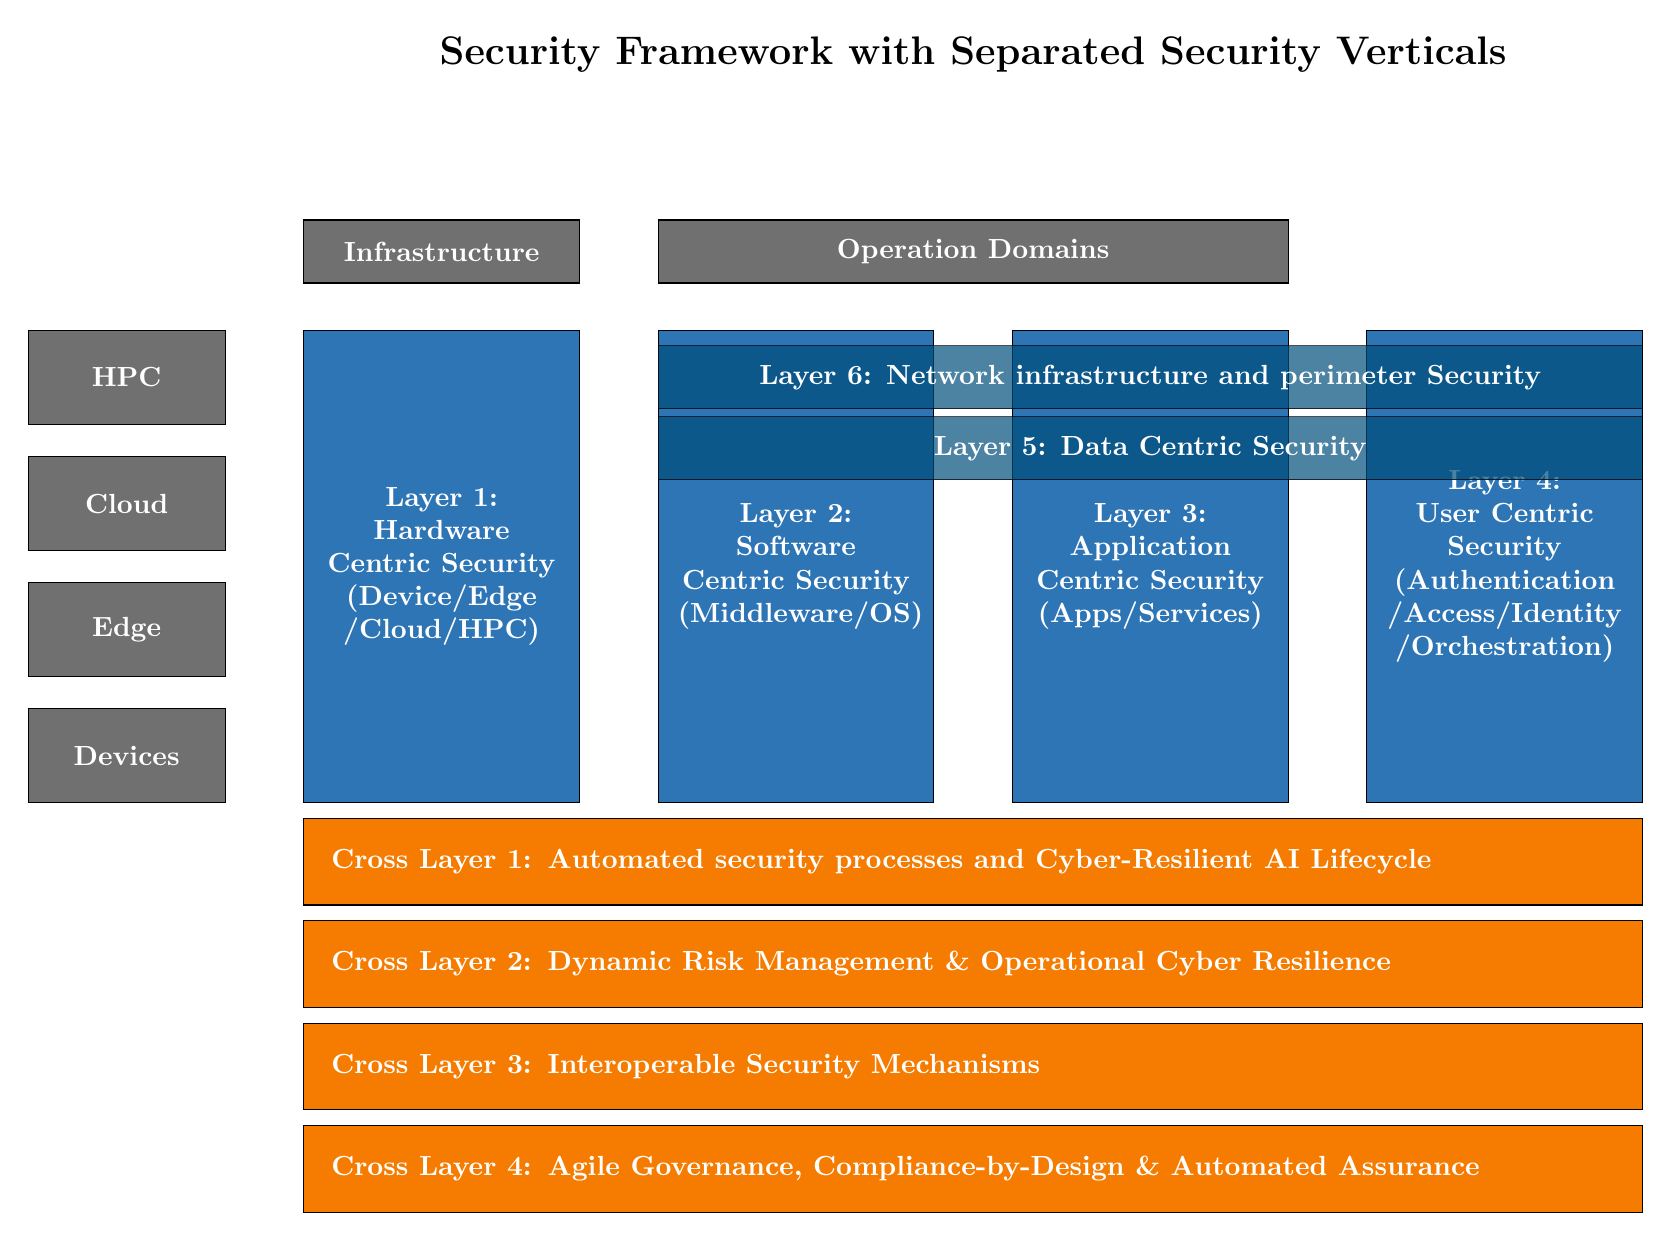
\begin{tikzpicture}[every node/.style={font=\small}]
			% Define colors
			\definecolor{archblue}{RGB}{46, 117, 182}
			\definecolor{sec_verticals_bg}{RGB}{245, 124, 0}
			\definecolor{env_bg}{RGB}{112, 112, 112}
			\definecolor{overlay}{RGB}{0, 77, 122}

			% Styles
			\tikzstyle{arch_col} = [fill=archblue, draw=black, text=white, font=\bfseries, minimum width=3.5cm, minimum height=6cm, align=center, text width=3cm]
			\tikzstyle{env_box} = [fill=env_bg, draw=black, text=white, font=\bfseries, minimum width=2.5cm, minimum height=1.2cm, align=center]
			\tikzstyle{top_tool} = [draw=black, fill=env_bg, text=white, minimum height=0.8cm, align=center, font=\bfseries]
			\tikzstyle{overlay_box} = [fill=overlay, draw=black, text=white, font=\bfseries, minimum height=0.8cm, align=center, opacity=0.7, text opacity=1]
			\tikzstyle{vertical_box} = [fill=sec_verticals_bg, draw=black, text=white, font=\bfseries, minimum width=17.0cm, minimum height=1.1cm, align=left, text width=16.3cm]

			% Column X positions
			\def\colone{-4.5}
			\def\coltwo{0}
			\def\colthree{4.5}
			\def\colfour{9}
            \pgfmathsetmacro{\layerSpanLeft}{\coltwo-1.75}
            \pgfmathsetmacro{\layerSpanRight}{\colfour+1.75}
            \pgfmathsetmacro{\layerSpanCenter}{(\layerSpanLeft+\layerSpanRight)/2}
            \pgfmathsetmacro{\layerSpanWidth}{\layerSpanRight-\layerSpanLeft}

			% Environment boxes (left)
			\node[env_box] at (-8.5, 2.4) {HPC};
			\node[env_box] at (-8.5, 0.8) {Cloud};
			\node[env_box] at (-8.5, -0.8) {Edge};
			\node[env_box] at (-8.5, -2.4) {Devices};

			% Main architecture columns representing layers
			\node[arch_col] (hw) at (\colone, 0) {Layer 1: \\ Hardware Centric Security \\ (Device/Edge\\ /Cloud/HPC)};
			\node[arch_col] (mw) at (\coltwo, 0) {Layer 2: \\ Software Centric Security \\ (Middleware/OS)};
			\node[arch_col] (app) at (\colthree, 0) {Layer 3: \\ Application Centric Security \\ (Apps/Services)};
			\node[arch_col] (user) at (\colfour, 0) {Layer 4: \\ User Centric Security \\ (Authentication\\ /Access/Identity\\ /Orchestration)};

			% Top tooling boxes
			\node[top_tool, minimum width=3.5cm] at (\colone, 4) {Infrastructure};
			\node[top_tool, minimum width=8cm] at (2.25, 4) {Operation Domains};

			% Arrows from tooling
			\draw[->, line width=2pt, white] (\colone, 3.5) -- (\colone, 3.1);
			\draw[->, line width=2pt, white] (2.25, 3.5) -- (2.25, 3.1);

			% Other layers as overlays/headers
			\node[overlay_box, minimum width=12.5cm] at (4.5, 1.5) {Layer 5: Data Centric Security};
            \node[overlay_box, minimum width=\layerSpanWidth cm] at (\layerSpanCenter, 2.4) {Layer 6: Network infrastructure and perimeter Security};

			% Separated vertical boxes
			\node[vertical_box] at (2.25, -3.75) {\textbf{Cross Layer 1: Automated security processes and Cyber-Resilient AI Lifecycle}};
			\node[vertical_box] at (2.25, -5.05) {\textbf{Cross Layer 2: Dynamic Risk Management \& Operational Cyber Resilience}};
			\node[vertical_box] at (2.25, -6.35) {\textbf{Cross Layer 3: Interoperable Security Mechanisms}};
			\node[vertical_box] at (2.25, -7.65) {\textbf{Cross Layer 4: Agile Governance, Compliance-by-Design \& Automated Assurance}};

			% Title
			\node[font=\Large\bfseries, anchor=center] at (2.25, 6.5) {Security Framework with Separated Security Verticals};

		\end{tikzpicture}%
		}
		\caption{Security Framework with separated security verticals in dedicated boxes.}
		\label{fig:security_framework_verticals_boxes}
    \end{figure*}


The roadmap is developed through a structured five-stage analytical pipeline
(Figure~\ref{fig:security_framework_verticals_boxes}). Each stage has a clearly defined
input, transformation logic, and output, ensuring that the final strategic
recommendations are fully traceable back to the architectural framework and
threat landscape.


The architectural framework presented in
Figure~\ref{fig:security_framework_verticals_boxes}
serves as the formal reference model of this roadmap.
It defines the logical structure of cybersecurity capabilities
across the Cloud--Edge--IoT continuum and provides the structured
methodological basis from which candidate capabilities are derived
for prioritization.


\begin{enumerate}
\item \textbf{Stage~1 -- Capability Identification:}
Using the architectural framework as the structured reference model,
this stage systematically identifies and enumerates the cybersecurity
capabilities required across the Cloud--Edge--IoT continuum.
The framework organizes these capabilities into six vertical Security
Layers and four transversal Cross-Layers, ensuring comprehensive
coverage of technical, operational, and governance functions.
Each sub-item within this framework constitutes a distinct
\emph{candidate capability} that enters the prioritization pipeline.

    \item \textbf{Stage~2 -- 7-Dimensional Capability Profile:}
    Each Executive Priority is analyzed in depth through a seven-dimension
    template, producing a complete, actionable R\&I profile: where Europe
    stands today, what must be built, why it is urgent, how to get there,
    what could go wrong, and how the system survives failure
    (Section~\ref{sec:7dim}).

    \item \textbf{Stage~3 -- Progression Matrix and Cross-Priority Phase
    Synthesis:}
    Each priority's 7-dimensional profile is condensed into a three-phase
    progression matrix tracking two objective metrics: Operational Deployment
    Phase (ODP) and Strategic Sovereignty Level (SSL). The matrices are then
    read \emph{across} all priorities per phase to identify shared enablers,
    cross-cutting risks, and aggregate strategic postures for each time horizon
    (Section~\ref{sec:matrix}).

    \item \textbf{Stage~4 -- 4-Filter Prioritization:}
    Each candidate priority is assessed against four filters. Priorities
    satisfying the highest number of filters, and in particular satisfying
    Filters~1 or~2 as mandatory conditions, are elevated to
    \emph{Executive Priorities}. The output of this stage is an ordered
    set of priorities defining the Phase~1 critical investment path
    (Section~\ref{sec:filters}).

    \item \textbf{Stage~5 -- Executive Summary Synthesis:}
    The per-phase strategic postures produced in Stage~4, combined with the
    cross-phase execution principles, are synthesized into phase-specific
    strategic recommendations and measurable success metrics for presentation
    to European Commission evaluators, funding bodies, and Member State
    national cybersecurity agencies (Section~\ref{sec:exec}).
\end{enumerate}

% -----------------------------------------------------------------
\subsection{Stage 1: Candidate Capability Identification}
\label{sec:capability_identification}
% -----------------------------------------------------------------
The architectural framework presented in
Figure~\ref{fig:security_framework_verticals_boxes} serves a dual purpose:
it is both a reference architecture for the secure European computing
continuum \emph{and} the structured source from which candidate capabilities
are derived for prioritization.

Every named sub-item within the six Security Layers (Layers~1 through~6) and
the four Transversal Cross-Layers (CL1 through CL4) constitutes a distinct
\emph{candidate capability} with an independent security function, maturity
trajectory, and set of R\&I requirements. The two structural dimensions of
the framework impose an important ordering constraint on the pipeline:

\begin{itemize}
    \item \textbf{Vertical dependency (Layer hierarchy):} Lower layers provide
    cryptographic and physical anchors upon which higher layers depend. A
    capability in Layer~4 (Orchestration) cannot provide meaningful security
    guarantees unless the capabilities in Layers~1 and~2 are already
    trustworthy. This architectural dependency directly informs Filter~2
    of the prioritization stage.

    \item \textbf{Horizontal reach (Cross-Layer scope):} Cross-Layer
    capabilities are not confined to a single technical layer; they apply
    governance, automation, and interoperability functions \emph{across} the
    full stack. Their prioritization reflects their role as force-multipliers
    for multiple vertical capabilities simultaneously, which is directly
    assessed by Filters~3 and~4.
\end{itemize}

The complete enumeration of candidate capabilities is presented in
Section~\ref{sec:arch}. Every candidate that passes through Stage~2
retains its Layer or Cross-Layer identifier, ensuring full architectural
traceability throughout the roadmap.

% -----------------------------------------------------------------
\subsection{Stage 2: The 4-Filter Prioritization Framework}
\label{sec:filters}
% -----------------------------------------------------------------
To provide actionable guidance for Horizon Europe and European Cybersecurity
Competence Centre (ECCC) investment decisions, each candidate capability is
assessed against a structured four-filter logic. The objective is to identify
the \emph{critical-path} capabilities requiring immediate resource allocation
during Phase~1 (0--5 years).

The four filters are not applied as an all-or-nothing gate; rather, each
filter that a capability satisfies contributes a \emph{positive signal}.
Two classification rules apply:

\begin{itemize}
    \item A capability satisfying \textbf{Filter~1 or Filter~2} is
    unconditionally elevated to an Executive Priority, because regulatory
    non-compliance and architectural blocking both represent immediate,
    non-deferrable risks.
    \item A capability satisfying \textbf{Filters~3 and/or~4} but neither
    Filter~1 nor~2 is scheduled as a Phase~2 or Phase~3 priority, with its
    rank determined by the number of filters satisfied.
\end{itemize}

\begin{enumerate}

    \item \textbf{Filter~1: Regulatory Urgency (The ``Must-Do'' Filter)}
    \begin{itemize}
        \item \textbf{Question:} Is this capability required to meet imminent
        European regulatory obligations (NIS2~\cite{nis2}, Cyber Resilience
        Act~\cite{cra}, AI Act~\cite{aiact})?
        \item \textbf{Logic:} Capabilities whose absence by 2026--2027 results
        in market exclusion, systemic non-compliance, or critical infrastructure
        vulnerability are unconditionally elevated to Phase~1 priority. The
        enforcement timeline of the relevant regulation determines urgency:
        CRA product requirements, NIS2 incident reporting obligations, and AI
        Act high-risk system conditions each impose distinct, legally binding
        deadlines.
        \item \textbf{Output signal:} \emph{Mandatory -- Phase~1 (non-deferrable).}
    \end{itemize}

    \item \textbf{Filter~2: Foundational Dependency (The ``Blocker'' Filter)}
    \begin{itemize}
        \item \textbf{Question:} Do other security capabilities depend on this
        capability as an architectural prerequisite?
        \item \textbf{Logic:} Capabilities lower in the vertical stack (e.g.,
        Layer~1 Hardware Roots of Trust) must be established before higher-layer
        capabilities (e.g., Layer~4 Zero-Trust Orchestration or Layer~5
        Confidential Computing) can provide meaningful guarantees. A blocked
        dependency means that funding higher-layer capabilities before the
        lower-layer anchor exists wastes investment. The architectural layer
        numbering (Section~\ref{sec:capability_identification}) provides the
        formal precedence rule.
        \item \textbf{Output signal:} \emph{Mandatory -- Phase~1 (architectural
        prerequisite).}
    \end{itemize}

    \item \textbf{Filter~3: Strategic Sovereignty Risk (The ``Extinction'' Filter)}
    \begin{itemize}
        \item \textbf{Question:} Does the absence of this capability create a
        strategic dependency, systemic resilience gap, or technology cliff
        for European digital sovereignty?
        \item \textbf{Logic:} This filter identifies capabilities where
        (a)~Europe currently holds 100\% dependency on non-EU vendors, leaving
        critical infrastructure exposed to extra-territorial access and
        geopolitical leverage, or (b)~a foreseeable adversarial or technological
        breakthrough would render existing European defenses obsolete before
        countermeasures can be deployed. The ``sovereignty cliff'' designation
        applies when either condition is true and no credible EU-controlled
        fallback exists.
        \item \textbf{Output signal:} \emph{High priority -- Phase~1 or Phase~2
        depending on co-occurrence with Filters~1/2.}
    \end{itemize}

    \item \textbf{Filter~4: Market Feasibility \& Ecosystem Alignment
    (The ``Adoption'' Filter)}
    \begin{itemize}
        \item \textbf{Question:} Can this capability realistically be adopted
        by European industry---including SMEs---and does it align with and
        amplify existing EU investments (e.g., Simpl middleware
        \cite{cloud_edge_roadmap}, EU Chips Act, Digital Europe Programme)?
        \item \textbf{Logic:} Priority is given to capabilities that act as
        force-multipliers for existing European infrastructure, reducing
        duplication and ensuring economic viability for the full ecosystem.
        A capability with strong market feasibility but weak filter~1/2/3
        scores is deferred to a phase where adoption infrastructure is mature.
        \item \textbf{Output signal:} \emph{Amplifying factor -- influences
        phase placement and implementation sequencing.}
    \end{itemize}

\end{enumerate}

\noindent\textbf{Stage~2 Output:} The multi-filter assessment produces an
ordered set of \emph{Executive Priorities} --- the capabilities that define
the Phase~1 critical investment path --- plus a ranked backlog of Phase~2 and
Phase~3 capabilities. Each Executive Priority carries a filter-satisfaction
record that directly justifies its rank in the 7-dimensional profiles of
Stage~3. The current roadmap identifies ten Executive Priorities (detailed
in Section~\ref{sec:priorities}), with Priorities~1--3 satisfying the
highest number of filters and constituting the absolute critical path.

% -----------------------------------------------------------------
\subsection{Stage 3: The 7-Dimensional Capability Profile}
\label{sec:7dim}
% -----------------------------------------------------------------
Each Executive Priority produced by Stage~2 is translated into a complete,
evaluator-grade R\&I profile using a seven-dimension analytical template.
This template ensures that every capability is characterized not only
from a technical perspective but also in terms of its regulatory alignment, investment
pathway, failure modes, and contribution to European strategic autonomy.
The template is applied identically to every priority, enabling consistent
cross-priority comparison.

\begin{enumerate}

    \item \textbf{Dimension~1: Baseline \& Target Objective}\\
    \textit{Question: Where does Europe stand today, and what does success
    look like by 2040?}\\
    \textit{Purpose:} Grounds the priority in reality by capturing the current
    Operational Deployment Phase (ODP), Strategic Sovereignty Level (SSL),
    industrial capacity, and barriers to adoption. The target defines
    measurable end-states (target ODP, target SSL, quantified EU market share)
    that serve as the basis for funding project calls and Phase~4 synthesis.

    \item \textbf{Dimension~2: Primary Drivers}\\
    \textit{Question: Why must Europe build this capability now?}\\
    \textit{Purpose:} Articulates the external pressures---both adversarial and
    regulatory---that make this priority urgent and non-deferrable.
    \begin{itemize}
        \item \textbf{Threat Drivers:} Adversarial capabilities or attack
        vectors that are already active or imminently scalable.
        \item \textbf{Regulatory Drivers:} Specific EU legal obligations with
        enforcement timelines, citing the precise directive and relevant
        provisions.
    \end{itemize}

    \item \textbf{Dimension~3: High-Impact Activities}\\
    \textit{Question: Which specific technical interventions yield the greatest
    strategic return on investment?}\\
    \textit{Purpose:} Identifies 3--5 concrete, actionable R\&I activities
    within the capability area, each formulated as a specific, measurable
    initiative rather than a general goal. Activities are tagged with their
    target phase (Phase~1, 2, or 3) to ensure the progression matrix in
    Stage~4 is anchored in concrete work.

    \item \textbf{Dimension~4: Catalysts \& Enablers}\\
    \textit{Question: What specific EU funding, standards, and ecosystem support
    are required to accelerate from baseline to target?}\\
    \textit{Purpose:} Identifies the concrete pull mechanisms and investment
    vehicles needed to drive market adoption.
    \begin{itemize}
        \item \textbf{R\&I \& Funding Alignment:} Horizon Europe clusters,
        Digital Europe Programme calls, and ECCC Strategic Agenda work
        packages \cite{eccc}.
        \item \textbf{Regulatory \& Standardization:} Required CEN/CENELEC,
        ETSI, or ISO standards, distinguishing between existing standards to
        be referenced and new standards that must be developed.
        \item \textbf{Ecosystem Enablers:} Pilot infrastructure (e.g.,
        federated Cyber Ranges), industrial partnerships (e.g., Gaia-X,
        IPCEI-CIS), and SME capacity-building schemes.
    \end{itemize}

    \item \textbf{Dimension~5: Disruptors \& Systemic Risks}\\
    \textit{Question: What structural vulnerabilities, market failures, or
    adversarial breakthroughs could derail the capability trajectory?}\\
    \textit{Purpose:} Acknowledges that R\&I trajectories are non-linear by
    identifying the specific risks that could render planned deployments
    obsolete or unachievable. Three risk categories are assessed for each
    priority:
    \begin{itemize}
        \item \textbf{Technical Cliffs:} Moments when a defensive capability
        is rendered obsolete by an adversarial or technological breakthrough
        before the EU countermeasure is fully deployed (e.g., a cryptanalytic
        advance against a standardized algorithm before migration is complete;
        a side-channel attack class that bypasses current hardware enclave
        implementations).
        \item \textbf{Supply Chain \& Market Risks:} Fabrication bottlenecks,
        vendor resistance to open standards, monopolization of critical
        components by non-EU providers, or SME exclusion from certification
        pathways.
        \item \textbf{Geopolitical \& Regulatory Risks:} Export controls on
        critical components, extra-territorial jurisdiction conflicts, or
        fragmented national implementation undermining EU-wide interoperability.
    \end{itemize}

    \item \textbf{Dimension~6: Failsafe Mechanisms \& Resilience}\\
    \textit{Question: If this capability is compromised or delayed, how does
    the system survive and gracefully degrade?}\\
    \textit{Purpose:} The technical core of ``Cyber-Resilience'' as applied
    to the roadmap itself. It defines engineering fallbacks for each priority's
    primary mechanism. Four categories of failsafe must be addressed:
    \begin{itemize}
        \item \textbf{Hybrid Transitional Schemes:} Parallel deployment of the
        target technology alongside the incumbent (e.g., classical + PQC
        cryptography; proprietary TPM + RISC-V secure element) during the
        migration window.
        \item \textbf{Graceful Degradation:} The minimum viable operational
        mode the infrastructure can sustain if the primary capability is
        unavailable (e.g., cached credential operation during cloud
        disconnection; localized physical-layer authentication if
        cryptographic processing fails).
        \item \textbf{Autonomous Isolation Protocols:} Automated quarantine
        or revocation mechanisms that activate when a node or component fails
        attestation, preventing compromise propagation without human
        intervention.
        \item \textbf{Implementation Diversity:} Deliberate multi-vendor or
        multi-algorithm diversity to avoid monoculture vulnerabilities (e.g.,
        deploying two independent TEE architectures; supporting multiple
        NIST-standardized PQC algorithm families).
    \end{itemize}

    \item \textbf{Dimension~7: Transversal Meta-Layer (Policy Alignment)}\\
    \textit{Question: How does mastering this capability advance Europe's
    overarching goals of sovereignty, sustainability, and societal trust?}\\
    \textit{Purpose:} Elevates the technical capability profile to the
    political and societal level, connecting it to the EU's strategic
    autonomy agenda.
    \begin{itemize}
        \item \textbf{Sovereignty \& Autonomy:} Quantified reduction in
        extra-territorial technology dependencies; contribution to SSL
        progression.
        \item \textbf{Trust \& Ethics:} Alignment with GDPR, Privacy-by-Design,
        algorithmic transparency, and the AI Act's trustworthiness requirements.
        \item \textbf{Sustainable Security (Green IT):} Energy efficiency
        of cryptographic or monitoring operations; e-waste reduction through
        crypto-agility (eliminating hardware replacement); alignment with the
        EU Green Deal.
    \end{itemize}

\end{enumerate}

\noindent\textbf{Stage~3 Output:} A complete, 7-dimension capability profile
for each Executive Priority. The Baseline (Dimension~1) and High-Impact
Activities (Dimension~3) directly populate the \emph{Operational State} cells
of the Stage~4 Progression Matrix. The Critical Enablers (Dimension~4) populate
the matrix's \emph{Critical Enabler} row. Disruptors (Dimension~5) and
Failsafes (Dimension~6) inform the resilience provisions in the Phase
Synthesis and Executive Summary.

% -----------------------------------------------------------------
\subsection{Stage 4: Progression Matrix and Cross-Priority Phase Synthesis}
\label{sec:matrix}
% -----------------------------------------------------------------

\subsubsection*{4a.\ The Per-Priority Progression Matrix}
Rather than relying on subjective Technology Readiness Levels (TRL) for a
highly fragmented ecosystem, each capability profile is condensed into a
three-phase progression matrix using four objective, market-observable
indicators. The matrix columns correspond to the three strategic time
horizons; each row tracks a distinct dimension of maturity:

\begin{itemize}
    \item \textbf{Operational Deployment Phase (ODP):} Tracks the market
    reality and integration status of the capability across the EU ecosystem.
    The ODP scale progresses through four stages:
    \emph{Applied R\&D} (laboratory/prototype phase) $\rightarrow$
    \emph{Fragmented Piloting} (isolated national or sectoral pilots) $\rightarrow$
    \emph{Standardized Integration} (harmonized deployment across multiple
    providers and Member States) $\rightarrow$
    \emph{Ubiquitous Operation} (Security-by-Design default, manual
    configuration obsolete). A capability's \emph{starting} ODP in Phase~1
    is set by its Dimension~1 Baseline; the \emph{target} ODP in Phase~3
    is set by its Dimension~1 Target.

    \item \textbf{Strategic Sovereignty Level (SSL):} Tracks European
    strategic autonomy and dependency on non-EU technology vendors. The SSL
    scale progresses through three stages:
    \emph{High Foreign Dependency} (critical function relies on non-EU
    components with no credible EU alternative) $\rightarrow$
    \emph{Emerging EU Ecosystem} (EU alternatives exist at pilot or early
    production scale; hybrid EU/non-EU deployments) $\rightarrow$
    \emph{Full Sovereign Autonomy} (EU-designed components dominate the
    market; no critical extra-territorial dependency). SSL progression is
    gated by the concrete investments and fabrication milestones identified
    in Dimension~4.

    \item \textbf{Operational State:} A concise 2--3 sentence snapshot
    characterizing the practical reality ``on the ground'' during each phase:
    which deployments are active, what remains manual or incomplete, and
    what the dominant risk exposure is at that point in time.

    \item \textbf{Critical Enabler:} The single most important regulation,
    standard, or European R\&I breakthrough that must be achieved to
    \emph{unlock the transition} to the next phase. This is not a list of
    desirable inputs but the specific gate condition without which Phase
    transition cannot occur. It is derived directly from Dimension~4
    (Catalysts \& Enablers) and Dimension~5 (Disruptors) of the capability
    profile.
\end{itemize}

The three time horizons are defined as follows:

\begin{itemize}
    \item \textbf{Phase~1: Foundation \& Compliance (0--5 Years):}
    Focus on state-of-practice deployments, immediate regulatory compliance
    (NIS2, CRA enforcement), and bridging the most critical capability gaps.
    The ODP and SSL positions at the end of Phase~1 define the baseline for
    Phase~2 investment planning.

    \item \textbf{Phase~2: Federation \& Standardization (5--10 Years):}
    Focus on industrializing and federating Phase~1 pilots, establishing
    harmonized governance frameworks, and managing critical technology
    transitions (e.g., PQC migration, RISC-V silicon scale-up). Cross-border
    interoperability and pan-European certification systems become the primary
    integration challenge.

    \item \textbf{Phase~3: Autonomy \& Leadership (10--15 Years):}
    Focus on achieving full sovereign autonomy, deploying autonomous
    Security-by-Design architectures, and positioning European frameworks as
    global reference implementations. Residual Phase~2 transitions are
    completed; next-generation threat vectors (post-quantum, neuromorphic,
    space-based edge) are addressed.
\end{itemize}

\subsubsection*{4b.\ Cross-Priority Phase Synthesis}
The per-priority matrices are individual capability views. Before producing
the Executive Summary, the matrices must be read \emph{across} all priorities
within each phase to generate a \emph{phase-level strategic posture
assessment}. This cross-priority synthesis follows three analytical steps:

\begin{enumerate}
    \item \textbf{Shared Critical Enabler Identification:}
    The \emph{Critical Enabler} row is read across all priority matrices for
    a given phase. Enablers that appear for multiple priorities in the same
    phase (e.g., ``CRA enforcement'' appearing as the Phase~1 enabler for both
    Hardware Roots of Trust and Supply Chain Verification) are designated as
    \emph{cross-cutting investments} --- regulatory or funding actions with
    disproportionate leverage across the portfolio.

    \item \textbf{ODP/SSL Posture Aggregation:}
    The ODP and SSL positions across all priorities at the end of a given
    phase are reviewed collectively to identify:
    (a)~\emph{lagging capabilities} --- where ODP or SSL progression is
    significantly behind the portfolio median, indicating that a shared
    bottleneck (fabrication, standardization, political will) is constraining
    multiple priorities simultaneously;
    (b)~\emph{interdependency risks} --- where a Phase~2 capability's ODP
    starting point depends on a Phase~1 capability reaching a specific SSL
    level that is currently projected to be insufficient.

    \item \textbf{Phase Gate Assessment:}
    For each phase, the synthesis produces a single \emph{phase gate
    assessment}: a structured statement of (a)~the cross-cutting enabling
    actions that unlock the most capability transitions simultaneously,
    (b)~the primary shared risk that could stall the portfolio, and
    (c)~the aggregate ODP/SSL trajectory European infrastructure is on. This
    phase gate assessment is the direct input to Stage~5.
\end{enumerate}

\noindent\textbf{Stage~4 Output:} Three phase gate assessments (one per time
horizon) and an identified set of cross-cutting investments, both of which
feed directly into the Executive Summary recommendations.

% -----------------------------------------------------------------
\subsection{Stage 5: Executive Summary Synthesis}
\label{sec:exec}
% -----------------------------------------------------------------
The Executive Summary (Section~\ref{sec:executive_summary}) is not intended as a
standalone narrative but the direct output of the Stage~4 phase gate
assessments combined with the cross-phase execution principles.

Its structure maps one-to-one onto the pipeline outputs:
\begin{itemize}
    \item \textbf{Strategic Narrative:} Synthesizes the overall ODP/SSL
    trajectory across all priorities into a coherent description of the
    journey from today's fragmented, foreign-dependent posture to full
    sovereign autonomy.
    \item \textbf{Per-Phase Recommendations:} Each phase's
    cross-cutting investments (from Phase Synthesis, Step~1) are restated
    as actionable policy and funding directives for European Commission
    evaluators and Member State agencies.
    \item \textbf{Success Metrics:} The measurable targets stated in
    each priority's Dimension~1 (Target Objective) and the Phase~1/2/3
    ODP/SSL end-states from the matrices are aggregated into a unified set
    of per-phase success criteria, enabling objective evaluation by ECCC
    annual reviews.
    \item \textbf{Risk Register:} The primary shared risk identified in each
    Phase Gate Assessment is surfaced as a named strategic risk requiring
    cross-portfolio mitigation, not merely a per-priority concern.
\end{itemize}

\subsection{The Anatomy of a Roadmap Priority: A Hybrid 7-Dimensional Analysis Template}

To ensure the roadmap is actionable, realistic, and aligned with European strategic autonomy, each priority is analyzed through a hybrid 7-dimensional profiling framework that combines methodological consistency with contextual flexibility. The template is applied consistently across priorities, with the first four dimensions treated as mandatory and the remaining dimensions applied where relevant based on risk exposure, system criticality, and policy impact.

\subsubsection*{Priority Profiling Framework: Mandatory and Adaptive Dimensions}
To ensure both analytical rigor and flexibility across heterogeneous priorities, the 7-dimensional profiling framework is structured into:

\begin{itemize}
    \item \textbf{Mandatory Core Dimensions:} Applied to every priority to ensure comparability, traceability, and alignment with EU strategic objectives.
    \item \textbf{Adaptive Contextual Dimensions:} Applied selectively depending on the nature, maturity, and risk profile of each priority.
\end{itemize}

This hybrid approach ensures that all priorities are evaluated consistently, while allowing deeper analysis where complexity, uncertainty, or systemic risk requires it.

\subsubsection*{Dimension Applicability Logic}
Not all priorities require equal depth across all seven dimensions. Therefore:

\begin{itemize}
    \item The \textbf{first four dimensions are mandatory} and must be defined for every priority.
    \item The remaining three dimensions are \textbf{conditionally applied} based on:
    \begin{itemize}
        \item System criticality
        \item Exposure to systemic or adversarial risk
        \item Policy and societal relevance
    \end{itemize}
\end{itemize}

This ensures proportional analysis effort while maintaining methodological consistency.

\begin{table*}[!t]
\centering
\caption{Priority profiling dimensions and applicability}
\begin{tabular}{p{5cm} p{3cm} p{6cm}}
\toprule
\textbf{Dimension} & \textbf{Type} & \textbf{Purpose} \\
\midrule
Baseline \& Target Objective & Mandatory & Define maturity trajectory and target state \\
Primary Drivers & Mandatory & Establish urgency and justification \\
High Impact Activities & Mandatory & Identify key interventions \\
Catalysts \& Enablers & Mandatory & Define EU support mechanisms \\
Disruptors \& Risks & Adaptive & Identify systemic and adversarial threats \\
Failsafe Mechanisms \& Resilience & Adaptive & Ensure resilience under failure \\
Transversal Meta-Layer & Adaptive & Align with EU policy and societal goals \\
\bottomrule
\end{tabular}
\end{table*}

\begin{enumerate}
    \item \textbf{Baseline \& Target Objective (The Trajectory) - Q: Where do we stand today, and what exactly does success look like?}\\
    \textit{Description:} Establishes the starting point of the priority today and defines the ultimate maturity state required by the end of the 15-year roadmap.\\
    \textbf{Evaluation Output:} Defines the maturity gap and informs phase transition readiness.
    \begin{itemize}
    \item \textbf{Baseline (Where we are):} Grounds the roadmap in reality. It captures the state of the art, current Operational Deployment Phase (ODP), Strategic Sovereignty Level (SSL), industrial capacity, reliance on foreign vendors, and the technical or economic barriers preventing immediate adoption.
    \item \textbf{Target (Where we need to be):} Sets the baseline for EU-funded projects, defining the target ODP and SSL that must be achieved by the end of the roadmap.
\end{itemize}
    
    \item \textbf{Primary Drivers (The ``Push'' Factors) - Q: Why must we prioritize building this capability right now? SQ: Why are we doing this?}\\
    \textit{Description:} Outlines the external pressures---both from the evolving threat landscape and mandatory EU regulations---that make this technological evolution urgent and unavoidable.\\
    \textbf{Interpretation:} Determines urgency and influences prioritization ranking.
    \begin{itemize}
        \item \textbf{Threat Drivers:} The rapid advancement of adversarial capabilities (e.g., offensive AI, quantum decryption, supply chain targeting).
        \item \textbf{Regulatory Drivers:} Imminent EU compliance mandates that require technical operationalization (e.g., NIS2, Cyber Resilience Act, AI Act).
    \end{itemize}

    \item \textbf{High Impact Activities - Q: Which specific actions provide the greatest leap in European sovereignty and security? SQ: Which should be the key initiatives?}\\
    \textit{Description:} Highlights the specific, prioritized technical interventions within this broader capability group that will yield the highest strategic return on investment.\\
    \textbf{Output:} A shortlist of actionable R\&I and deployment interventions.

    \item \textbf{Catalysts \& Enablers (The ``Pull'' Factors \& EU Support) - Q: What specific EU funding, standards, and ecosystem support do we need? SQ: How do we get there \& accelerate?}\\
    \textit{Description:} Identifies the concrete mechanisms, funding vehicles, and regulatory standardizations required from the EU to accelerate market adoption and push the industry from the baseline to the target state.\\
    \textbf{Role in Methodology:} Bridges priorities with EU instruments, ensuring implementation feasibility.
    \begin{itemize}
        \item \textbf{R\&I \& Funding Alignment:} Required Horizon Europe funding topics and targeted innovation instruments. Investment priorities must be explicitly synchronized with the European Cybersecurity Competence Centre (ECCC) Strategic Agenda \cite{eccc} to ensure alignment with pan-European goals (e.g., PQC transition infrastructure, AI-driven security tools).
        \item \textbf{Regulatory \& Standardization:} Alignment with standard-setting bodies (CEN/CENELEC) and certification frameworks (e.g., EUCS, EUCC).
        \item \textbf{Ecosystem:} Support for ecosystem building, industrial partnerships, and capacity-building initiatives (e.g., federated Cyber Ranges) to upskill the workforce and ensure advanced security solutions are economically viable for SMEs.
    \end{itemize}

    \item \textbf{Disruptors \& Systemic Risks (The Roadblocks) - Q: What structural vulnerabilities, market failures, or adversary breakthroughs could derail us? SQ: What can break the path?}\\
    \textit{Description:} Acknowledges that innovation is not linear by identifying severe technical and architectural risks that could actively derail deployment. It places primary emphasis on ``Technical Cliffs''---moments where defensive capabilities are rendered obsolete by adversarial breakthroughs before countermeasures are fully deployed.\\
    \textbf{Trigger Condition:} Applied when the priority is exposed to technological discontinuities or adversarial asymmetry.
    \begin{itemize}
        \item \textbf{Cryptographic Obsolescence \& Migration Bottlenecks (The Primary Technical Risk):}
        \begin{itemize}
            \item \textit{The ``Q-Day'' Cliff:} The risk that Cryptographically Relevant Quantum Computers (CRQC) become operational before the EU completes its migration to Post-Quantum Cryptography (PQC). This creates a ``Harvest Now, Decrypt Later'' vulnerability.
            \item \textit{Migration Complexity:} The systemic failure to inventory and replace deep-rooted Public Key Infrastructure (PKI) in legacy OT/IoT environments.
        \end{itemize}
        \item \textbf{Adversarial Breakthroughs:} The risk of threat actors weaponizing emerging technologies (e.g., AI-driven exploit generation, polymorphic malware) faster than defensive R\&I can mitigate them.
        \item \textbf{Contextual Risks (Non-Technical / Optional):} Geopolitics \& supply chain dependencies, market \& technology risks (monopolization, fragmented standards).
    \end{itemize}

    \item \textbf{Failsafe Mechanisms \& Resilience (The Safety Nets) - Q: If this technology is compromised, how does the system survive and gracefully degrade? SQ: How do we prevent failure?}\\
    \textit{Description:} The technical core of ``Cyber-Resilience.'' It defines the engineering fallbacks required if a primary capability fails, is breached, or is disrupted by the systemic risks identified above.\\
    \textbf{Purpose:} Ensures continuity of operations under failure or compromise scenarios.\\
    \textbf{What it entails:} Designing for degraded modes of operation, architectural redundancies, autonomous isolation protocols, and implementation diversity to avoid vulnerable technological monocultures.

    \item \textbf{Transversal Meta-Layer (The Policy Alignment) - Q: How does mastering this capability support Europe's goals of sovereignty, sustainability, and trust? SQ: The broader policy context?}\\
    \textit{Description:} Elevates the technical capability back to the overarching political and societal goals of the European Union.\\
    \textbf{Strategic Role:} Aligns technical priorities with EU-wide policy narratives and long-term societal impact.
    \begin{itemize}
        \item \textbf{Sovereignty \& Autonomy:} Strengthening European strategic independence, reducing reliance on non-EU vendors.
        \item \textbf{Trust \& Ethics:} Fostering deep societal trust by guaranteeing data privacy (Privacy-by-Design), algorithmic fairness, and transparency.
        \item \textbf{Sustainable Security (Green IT):} Minimizing the environmental impact of cyber defense (e.g., energy-efficient cryptographic algorithms, crypto-agility to reduce e-waste).
    \end{itemize}
\end{enumerate}

\begin{table*}[!t]
\centering
\caption{Mapping from 7-Dimensional Profile to Progression Matrix}
\begin{tabular}{p{5cm} p{6cm}}
\toprule
\textbf{Profile Dimension} & \textbf{Matrix Component} \\
\midrule
Baseline \& Target Objective & ODP and SSL starting/target levels \\
High Impact Activities & Operational State evolution \\
Catalysts \& Enablers & Critical Enabler \\
Disruptors \& Risks & Phase risk considerations \\
Failsafe Mechanisms & Resilience assumptions in synthesis \\
\bottomrule
\end{tabular}
\end{table*}

\subsection{Phase Transition Mechanism - Progression Matrix: Sequence of Events (X-Axis)}

The roadmap is structured across multiple time phases (e.g., short-term, mid-term, long-term). Each phase represents a column in the prioritization matrix.

Transitions between phases are governed by the evolution of capabilities and priorities across these columns.

Instead of a strictly chronological timeline, the roadmap maps the sequence of critical events required to unlock maturity. This ensures that foundational capabilities are built before advanced autonomous systems.

\begin{itemize}
    \item \textbf{Phase 1: Foundation \& Compliance (Immediate Implementation):} Focuses on state-of-practice deployments, bridging immediate capability gaps, and addressing urgent regulatory obligations (NIS2, CRA).
    \item \textbf{Phase 2: Federation \& Standardization (Scaling \& Harmonization):} Focuses on deploying emerging technologies, establishing harmonized governance frameworks, and managing critical transition periods.
    \item \textbf{Phase 3: Autonomy \& Leadership (Sovereign Innovation):} Focuses on highly speculative but structured foresight, including defense against quantum-capable adversaries and the achievement of fully sovereign, autonomous cloud-edge ecosystems.
\end{itemize}



For each phase:

\begin{itemize}
    \item Input: Set of prioritized capabilities from the previous phase
    \item Processing: Application of the 4-dimensional filtering logic
    \item Output: Updated set of priorities for the next phase
\end{itemize}

A transition occurs when:

\begin{itemize}
    \item A capability increases in maturity or feasibility
    \item Dependencies are resolved
    \item Regulatory pressure increases
    \item Strategic importance shifts
\end{itemize}

Each transition produces a \textbf{phase summary}, capturing:

\begin{itemize}
    \item Newly introduced priorities
    \item Evolved priorities
    \item Deferred or dropped priorities
\end{itemize}

\subsection*{Matrix Cell Content Definition (Measuring Progression)}
Rather than relying on subjective Technology Readiness Levels (TRL) or Manufacturing Readiness Levels (MRL) for a highly fragmented ecosystem, each cell in the progression matrix tracks maturity using objective strategic market and policy indicators:

\begin{itemize}
    \item \textbf{Operational Deployment Phase (ODP):} Tracks the market reality and integration status (e.g., \textit{Applied R\&D $\rightarrow$ Fragmented Piloting $\rightarrow$ Standardized Integration $\rightarrow$ Ubiquitous Operation}).
    \item \textbf{Strategic Sovereignty Level (SSL):} Tracks European strategic autonomy and reliance on foreign vendors (e.g., \textit{High Foreign Dependency $\rightarrow$ Emerging EU Ecosystem $\rightarrow$ Full Sovereign Autonomy}).
    \item \textbf{Operational State:} A concise snapshot characterizing the reality on the ground during this phase.
    \item \textbf{Critical Enabler:} The single most critical regulation, standard, or European R\&I breakthrough unlocking the transition to the next phase.
\end{itemize}

\subsection{From Priorities to Executive Summary: Final Strategic Synthesis}

After priorities are profiled and their cross-phase progression is captured in the transition matrix, a final synthesis step is applied to convert detailed technical analysis into executive-level strategic guidance.

The synthesis is non-normative and evidence-driven, relying exclusively on outputs generated in previous stages rather than introducing new assumptions.

This synthesis does not re-score priorities. Instead, it aggregates the strongest signals emerging from the previous methodological steps and translates them into decision-oriented messages for policymakers, funders, and industrial stakeholders.

\subsubsection*{Inputs to the Synthesis Step}
The final synthesis reads and consolidates the following inputs:
\begin{itemize}
    \item The selected \textbf{Executive Priorities} emerging from the 4-filter logic
    \item The \textbf{mandatory and adaptive dimensions} captured in each priority profile
    \item The \textbf{cross-phase evolution} recorded in the progression matrices, including ODP, SSL, operational state, and critical enablers
\end{itemize}

\subsubsection*{Synthesis Logic}
This step defines the \textbf{aggregation logic} of the methodology, transforming individual priority analyses into system-level strategic insights.
The synthesis step identifies:
\begin{itemize}
    \item \textbf{Common patterns} across priorities (e.g., repeated dependencies on hardware trust, PQC migration, interoperability, or compliance automation)
    \item \textbf{Cross-cutting bottlenecks} that appear in multiple priorities and therefore require coordinated EU action
    \item \textbf{Strategic inflection points} where delays in one capability would cascade into multiple downstream priorities
    \item \textbf{Investment signals} indicating where Horizon Europe, Digital Europe, ECCC, or standardization efforts should be concentrated
\end{itemize}

\subsubsection*{Output of the Synthesis Step}
The output of this step is an executive summary that distills the roadmap into:
\begin{itemize}
    \item A concise set of \textbf{critical strategic messages}
    \item A \textbf{prioritized investment narrative} for Phase 1 and beyond
    \item A \textbf{policy-aligned explanation} of why these priorities matter for sovereignty, resilience, and trust
\end{itemize}

This ensures that the executive summary is fully traceable to the analytical pipeline rather than functioning as a standalone narrative.
\subsection{Executive Summary as Aggregated Output}

The executive summary represents the final synthesis of the methodology and the output of the strategic synthesis step. It is not an independent narrative, but a structured aggregation of:

\begin{itemize}
    \item High-priority capabilities (from filtering)
    \item Cross-phase evolution trends (from transitions)
    \item Strategic gaps and investment needs
\end{itemize}

It provides:

\begin{itemize}
    \item A consolidated view of critical priorities
    \item Recommendations for R\&I funding and policy alignment
    \item Identification of strategic dependencies and risks
\end{itemize}

This ensures full traceability from raw capabilities to strategic recommendations.


\newpage
\section{Capabilities (Architectural Framework)}
\label{sec:arch}


As it is illustrated in Figure~\ref{fig:security_framework_verticals_boxes}, the roadmap is structured across a cohesive architectural framework that spans four continuum environments (HPC, Cloud, Edge, Devices). The capabilities are organized into Six Security Layers (The Vertical Stack) and Four Transversal Cross-Layers (The Horizontal Enablers).

\subsection*{Part A: The Security Layers (Vertical Stack)}
These layers define the specific technical security controls implemented across the computing infrastructure.

\subsubsection*{Layer 1: Hardware-Centric Security}
\textbf{1.1 Hardware Roots of Trust:} Cryptographically verifiable supply chain trust (e.g., TPM attestation, secure enclaves) ensures physical device integrity. Success depends on driving European open-hardware designs (e.g., RISC-V) toward \textbf{EUCC 'High' assurance level certification} \cite{eucc} to mathematically guarantee resistance against state-level physical tampering and side-channel attacks at the vulnerable far-edge.
\textbf{1.2 Physical-Layer (PHY) Threat Detection \& Fingerprinting:} Exploiting intrinsic wireless channel characteristics, such as Channel State Information (CSI), Carrier Frequency Offset (CFO), and Received Signal Strength Indicator (RSSI). That is to establish real-time, keyless device authentication and anomaly detection at the lowest layer of the stack. This provides a hardware-anchored security primitive that is resilient even when upper-layer cryptographic processing is compromised or infeasible.

\subsubsection*{Layer 2: Software-Centric Security (Middleware/OS)}

\textbf{2.1 OS \& Middleware Hardening:} Securing hypervisors, container runtimes, and distributed operating systems is critical for isolation. This involves hardening KVM/QEMU and supporting sovereign, lightweight Linux distributions optimized for edge resource constraints, ensuring a reduced attack surface for the cognitive continuum.

\textbf{2.2 Secure OTA Patch \& Update Management:} Edge nodes deployed in the field---smart grids, O-RAN radios, industrial gateways---require cryptographically verified, failure-resilient over-the-air (OTA) update pipelines. A compromised or failed update mechanism can render entire fleets of field-deployed nodes permanently vulnerable, making robust OTA management a critical software-layer capability.

\subsubsection*{Layer 3: Application-Centric Security (Apps/Services)}

\textbf{3.1 Workload Security:} Securing containerized applications, microservices, and serverless functions executing dynamically across multi-provider nodes. This is achieved through hardened service meshes and sidecar proxy architectures that provide mutual TLS and granular traffic inspection without impacting performance.

\textbf{3.2 In-Band Network Telemetry (INT) \& Deep Observability:} Embedding ``smart telemetry'' directly into the data packets traversing containerized workloads and service meshes, providing granular, real-time visibility into network behaviour and performance without requiring out-of-band monitoring infrastructure. This feeds high-fidelity signals to security analytics platforms.

\textbf{3.3 API Security Gateway \& Policy Enforcement:} As containerized AI workloads increasingly communicate through REST/gRPC APIs, a dedicated API security gateway provides a unified enforcement point for authentication tokens, rate limiting, schema validation, and payload inspection---preventing injection attacks and data exfiltration at the application boundary.


\subsubsection*{Layer 4: User \& Orchestration-Centric Security}
\textbf{4.1 Zero-Trust Orchestration:} Seamless policy enforcement across a multi-provider computing continuum requires robust Policy Enforcement Point (PEP) and Policy Decision Point (PDP) architectures. This enables continuous authorization and dynamic access controls that adapt to the context of the request.

\textbf{4.2 Federated Identity \& Access Management (IAM):} Cross-domain identity federation and verifiable credentials for machines, users, and automated workloads. Implementing \textbf{Self-Sovereign Identity (SSI)} principles allows for cryptographically secure, decentralized authentication across heterogeneous cloud-edge domains.

\textbf{4.3 Privileged Access Management (PAM) \& Just-In-Time (JIT) Access:} Lateral movement by attackers frequently exploits over-provisioned standing privileges---the precise vector behind major Advanced Persistent Threat (APT) campaigns. PAM and JIT access controls ensure that elevated privileges are granted only for defined, time-bounded sessions with full auditability, minimizing the blast radius of any credential compromise.

\subsubsection*{Layer 5: Data-Centric Security}
\textbf{5.1 End-to-end Confidential Computing:} Data-in-use security through Trusted Execution Environments (TEEs) spanning the entire Cloud-to-IoT data path. Leveraging TEE abstraction layers and remote attestation ensures that sensitive European data remains encrypted even during processing in non-trusted environments.

\textbf{5.2 Post-Quantum \& Cryptographic Agility:} PQC standardization and hybrid crypto deployment are necessary to secure long-lived data. Priority is placed on \textbf{PQC migration for resource-constrained devices}, ensuring that edge infrastructure is resilient against ``Harvest Now, Decrypt Later'' quantum threats.

\textbf{5.3 Signaling (Data) Security:} Moving beyond best-effort packet forwarding by embedding trust directly into the network signaling architecture. This ensures the integrity and authenticity of control-plane messages, preventing hijacking of routing decisions and network configuration across the distributed continuum.

\textbf{5.4 Distributed Reputation \& Trust Networking:} Implementing a ubiquitous, real-time reputation system built on Distributed Ledger Technology (DLT) and smart contracts. This enables autonomous, evidence-based trust decisions about nodes, services, and data sources across the continuum without reliance on a central authority.

\textbf{5.5 Quantum Key Distribution (QKD) for Critical Links:} While PQC addresses algorithmic quantum-resistance, QKD provides information-theoretically secure key exchange over optical fibre for point-to-point high-value links (government, critical infrastructure backbone). These two technologies are complementary and together form a comprehensive quantum-safe strategy.

\textbf{5.6 Secure Multi-Party Computation (SMPC):} Homomorphic Encryption and TEEs (Layer 5.1) handle confidential computing for single-party workloads. SMPC enables multiple mutually distrusting parties to jointly compute a function over their combined private inputs without revealing those inputs to each other---a critical capability for cross-border analytics and federated AI in regulated sectors.

\subsubsection*{Layer 6: Network Infrastructure \& Perimeter-Centric Security}
\textbf{6.1 Telco-cloud \& O-RAN Security:} Hardening distributed 5G/6G cores and RAN components must align with the \textbf{Smart Networks and Services Joint Undertaking (SNS JU) SRIA} \cite{snsju}. This ensures sovereign control over network slice isolation and virtualized RAN components.

\textbf{6.2 Cross-Sector Physical Resilience \& Safety:} Adapting strict network controls and IT/OT gateway security for high-availability edge environments (e.g., Smart Grids). This guarantees that cyber-breaches in the digital layer do not cascade into physical safety hazards or kinetic damage in critical infrastructure.

\textbf{6.3 Edge-Native Autonomous Guardians:} Hosting lightweight, localized security control functions (Security-as-a-Service aggregators) directly at the far-edge gateways or within Open-RAN Radio Intelligent Controllers (RIC). These autonomous guardian nodes execute real-time threat mitigation without requiring round-trip communication to a centralized cloud-based SOC, dramatically reducing response latency.

\textbf{6.4 Non-Terrestrial Network (NTN) \& Satellite Security:} 6G will natively integrate satellite segments for coverage continuity, backhaul resilience, and emergency operations. These non-terrestrial links introduce distinct threat surfaces---including signal interception and orbital spoofing---requiring dedicated security requirements aligned with 3GPP NTN specifications and the EU Space Programme.

\subsection*{Part B: The Transversal Security Verticals (Cross-Layers)}
These four cross-layers represent continuous, automated processes and governance structures that intersect every layer of the vertical stack.

\subsubsection*{Cross-Layer 1: Automated Security Processes \& Cyber-Resilient AI Lifecycle}
\textbf{CL1.1 Continuous DevSecOps (Shift-Left):} Embedding AI-driven code analysis and automated vulnerability remediation at the earliest stages of the software lifecycle.

\textbf{CL1.2 Model \& Pipeline Integrity (DataBOMs):} Securing AI training pipelines to prevent data poisoning and unauthorized model manipulation.

\textbf{CL1.3 Runtime AI Defense:} Defending AI/ML infrastructure against real-world adversarial attacks (e.g., prompt injection, model evasion/theft) at the edge.

\textbf{CL1.4 Dynamic Supply Chain Verification (Runtime SBOMs):} Moving beyond static software manifests by implementing dynamic Software Bill of Materials (Runtime SBOMs) and ``cryptographic proof of execution'' to continuously verify the integrity of containerized microservices and AI components as they migrate across the multi-provider edge-cloud continuum.

\textbf{CL1.5 Automated Adversarial Testing \& Continuous Purple Teaming:} DevSecOps pipelines focus on code analysis and remediation; the adversarial counterpart provides continuous automated penetration testing, fuzzing (coverage-guided and protocol-level), and purple-team automation that simulates real attacker behaviour against live staging environments, ensuring defenses are validated continuously rather than at periodic intervals.


\subsubsection*{Cross-Layer 2: Dynamic Risk Management \& Operational Cyber Resilience}
\textbf{CL2.1 Automated SOC Operations \& Collaborative Threat Intelligence:} Continuous monitoring, SOC federation across Member States, and automated incident containment, underpinned by legally protected, cross-border threat intelligence sharing ecosystems designed to overcome institutional trust barriers and incentivize active collaboration \cite{concordia}.

\textbf{CL2.2 Systemic \& Cascading Risk Mitigation:} Mapping the evolving threat landscape and using impact-likelihood scoring to dynamically sever links and prevent cross-domain systemic failures.

\textbf{CL2.3 High-Precision Telemetry and Security Signalling:} Implementing ``smart telemetry'' and cybersecurity-related signalling to feed real-time threat intelligence into analytics platforms without overwhelming network bandwidth---ensuring that visibility does not itself become an attack vector or performance bottleneck.

\textbf{CL2.4 Internet of Behavior (IoB) and Evidence Sharing:} Utilizing cybersecurity and QoS signalling traffic to extract and share behavioral patterns across the infrastructure, establishing an ``Internet of Behavior'' that enables proactive anomaly correlation and evidence-based risk assessment at continental scale.

\textbf{CL2.5 AI-Native Analytics Integration (NWDAF \& LLMSecOps):} Routing cybersecurity signalling traffic and telemetry through centralized analytics hubs powered by AI agents. This creates a live ``nervous system'' for the network, allowing AI agents to continuously monitor for zero-day exploits, analyze encrypted traffic flows, and trigger automated incident responses aligned with NWDAF (Network Data Analytics Function) standards.

\textbf{CL2.6 Cyber Threat Intelligence (CTI) Lifecycle Management:} While CL2.1 and CL2.4 consume and act on threat data, explicit governance of the full CTI lifecycle---collection, processing, analysis, dissemination, and feedback---is required as a prerequisite for the federated SOC vision. A sovereign EU CTI platform must define this governance layer to ensure data quality, legal compliance, and attribution reliability.

\textbf{CL2.7 Cyber Deception Technology \& Active Defense (Honeynets, Canaries):} Current detection is passive---telemetry is observed and anomalies flagged. Deception adds an active intelligence-collection dimension by deploying decoy assets (honeypots, honeynets, credential canaries, fake API endpoints) that generate high-fidelity, low-noise alerts when touched, enabling early detection of advanced intrusions and insider threats.

\subsubsection*{Cross-Layer 3: Interoperable Security Mechanisms \& Open-Source Verifiability}
\textbf{CL3.1 Heterogeneous Interoperability \& Simpl Integration:} Secure communication and data exchange across disparate systems, edge nodes, and proprietary domains. This includes mandatory alignment with and integration into the Simpl open-source smart middleware \cite{cloud_edge_roadmap} to ensure secure, federated access across Common European Data Spaces.

\textbf{CL3.2 Minimal Interoperability Mechanisms (MIMs) \& Open Verifiability:} Establishing standardized, baseline security and privacy controls to ensure trust without creating vendor lock-in. This relies heavily on embracing open-source software and open hardware architectures as fundamental prerequisites for transparency, cryptographic verifiability, and the elimination of proprietary black-box vulnerabilities \cite{cloud_edge_roadmap}.

\textbf{CL3.3 Neutral Host and Multi-Tenant Isolation:} As the ecosystem shifts toward infrastructure sharing and Neutral Host models spanning wireless, optical, and cloud domains, robust isolation between tenants is critical. Security architectures must enforce Zero-Trust edge operations across different network partitions to prevent cross-tenant data leakage and privilege escalation.

\textbf{CL3.4 Pan-European NaaS Federation and Cross-Border Edge Roaming:} Establishing standardized interfaces and harmonized Network APIs (e.g., leveraging CAMARA) to interconnect the fragmented edge clouds of different European telecom operators into a unified Network-as-a-Service (NaaS) platform---enabling a ``Schengen for Cloud/AI'' where compute workloads can roam seamlessly across borders.

\textbf{CL3.5 Semantic Security Interoperability (Common Ontologies \& Data Models):} Federated SOCs and shared threat intelligence only function if participating organisations share a common semantic understanding of security events, asset taxonomies, and risk classifications. Standardized ontologies (e.g., aligned with STIX/TAXII and MITRE ATT\&CK) are a prerequisite for meaningful cross-border correlation.

\textbf{CL3.6 Cyber Range \& Digital Twin Federation for Security Validation:} Before deploying cross-border federated security configurations into production, they must be validated in high-fidelity simulation environments. ENISA already coordinates national cyber range inventories; this cross-layer would federate them into a shared EU-wide infrastructure aligned with the Cyber Solidarity Act's testing provisions.

\subsubsection*{Cross-Layer 4: Compliance-by-Design, Agile Governance \& Automated Assurance}
\textbf{CL4.1 Policy-as-Code \& Compliance-by-Design:} Technical implementation of legal requirements (OSCAL) into machine-readable rules that pre-validate workloads.

\textbf{CL4.2 Continuous Automated Auditing \& Certification Lifecycle:} Replacing ``point-in-time''  PDF certificates with real-time, telemetry-driven certification tracking for both cloud services (EUCS) \cite{eucs} and physical ICT edge products (EUCC) \cite{eucc}. This ensures that edge nodes autonomously maintain compliance by integrating mandatory vulnerability handling and cryptographic patch verification directly into their operational lifecycle, strictly aligning with EUCC maintenance and assurance rules \cite{eucc}.

\textbf{CL4.3 Post-Quantum Readiness \& Zero-Trust Architectures (ZTA):} Moving beyond traditional perimeter-based defenses by embedding continuous, AI-driven Zero-Trust verification and micro-segmentation natively into the cloud-edge infrastructure, combined with a systematic migration roadmap to post-quantum cryptographic primitives across all layers.

\textbf{CL4.4 Continuous Automated Certification:} Replacing ``point-in-time'' PDF certificates with real-time, telemetry-driven certification tracking for both cloud services (\textbf{EUCS}) and physical ICT edge products (\textbf{EUCC}), ensuring that edge nodes autonomously maintain compliance by integrating mandatory vulnerability handling and cryptographic patch verification directly into their operational lifecycle \cite{eucc}.

\textbf{CL4.5 Multicloud Key Management as a Service (KMaaS):} When AI workloads, data flows, and context flows migrate dynamically across a multi-provider computing continuum, managing cryptographic keys and access policies becomes highly complex. KMaaS provides a provider-agnostic, sovereign key lifecycle management capability that prevents key sprawl and ensures revocation propagates consistently across heterogeneous environments.

\textbf{CL4.6 Privacy-Preserving Federated Computation:} When multiple providers work on the same infrastructure, AI training and inference may require access to datasets stored across different jurisdictions and competitive boundaries. Privacy-preserving techniques (federated learning, differential privacy, SMPC) enable collaborative computation while guaranteeing that raw data never leaves its sovereign jurisdiction.

\textbf{CL4.7 Cyber Risk Quantification \& Board-Level Reporting (CRQ):} Compliance frameworks define what controls to implement. A dedicated cross-layer translates technical security posture into financial and operational risk language for decision-makers---potentially in real-time---enabling boards to make informed, evidence-based investment and risk-acceptance decisions aligned with DORA requirements.

\textbf{CL4.8 AI Trustworthiness \& Algorithmic Accountability:} As AI systems themselves become actors within the security architecture---making autonomous containment decisions, classifying threats, orchestrating responses---the trustworthiness of those AI systems becomes a security-critical concern. This layer defines explainability, auditability, and override mechanisms for AI-driven security functions, ensuring alignment with the EU AI Act for high-risk systems.

\textbf{CL4.9 Regulatory Digital Twins:} Virtualized replicas of critical infrastructure specifically to stress-test regulatory compliance against evolving laws before applying changes to the live physical continuum.


\newpage

\section{Priorities}
\label{sec:priorities}
\subsection{Executive Priorities: The Critical Path (Phase 1)}
Applying the 4-Filter Framework, the following areas are identified as immediate strategic priorities for the 2025-2030 funding cycle:
\begin{itemize}
    \item \textbf{Priority 1:} Hardware Roots of Trust \& EUCC 'High' Certification (Filters 1, 2, 3).
    \item \textbf{Priority 2:} Post-Quantum Cryptographic Agility for Edge/IoT (Filter 3).
    \item \textbf{Priority 3:} Lightweight Cryptography \& Physical-Layer Security (PhySec) for the Extreme Edge.
    \item \textbf{Priority 4:} Security Interoperability via Simpl Middleware (Filter 4).
    \item \textbf{Priority 5:} Supply Chain Verification and Secured Infrastructure.
    \item \textbf{Priority 6:} Cognitive SecOps (LLMSecOps) \& Automated Threat Intelligence.
    \item \textbf{Priority 7:} Pan-European NaaS Federation (``Schengen for Cloud-Edge/AI'').
    \item \textbf{Priority 8:} Confidential Computing \& Privacy-Preserving AI Pipelines.
    \item \textbf{Priority 9:} Resilient-by-Design Infrastructure \& Autonomous ``Island Mode.''
    \item \textbf{Priority 10:} Proactive Cyber Threat Management \& Defense against Advanced Persistent Threats (APTs).
\end{itemize}

\section{Capability Profiles \& Progression Matrices}

% -----------------------------------------------------------------------
\subsection*{Priority 1: Hardware Roots of Trust \& EUCC 'High' Certification}
% -----------------------------------------------------------------------

\begin{enumerate}
\item \textbf{Baseline \& Target Objective:}
\textit{Baseline:} High foreign dependency on proprietary Trusted Platform Modules (TPMs) and secure elements. Far-edge devices lack standardized hardware anchors.
\textit{Target:} Ubiquitous deployment of EU-designed, open-source (RISC-V) secure enclaves certified at \textbf{EUCC 'High' assurance}, providing a mathematically verifiable foundation for the entire continuum.

\item \textbf{Primary Drivers:} 
\textit{Threat:} State-level physical tampering and side-channel attacks on decentralized edge nodes. 
\textit{Regulatory:} Mandatory hardware security requirements under the \textbf{Cyber Resilience Act (CRA)} and certified anchors for \textbf{NIS2} critical infrastructure.

\item \textbf{High Impact Activities:} 
Development of sovereign European Secure Elements based on RISC-V; automated hardware-level remote attestation protocols for large-scale edge fleets; EU-level standard toolset developed and maintained by the European Commission; SME support for certification and compliance testing; security-based sensor research for future deployment.

\item \textbf{Catalysts \& Enablers:} 
\textbf{EU Chips Act} pilot lines for secure silicon; \textbf{ECCC Strategic Agenda} funding for open-hardware security; alignment with CEN/CENELEC hardware security standards.

\item \textbf{Disruptors \& Systemic Risks:} 
Supply chain bottlenecks for EU-based fabrication; breakthroughs in physical side-channel analysis that bypass current cryptographic enclaves.

\item \textbf{Failsafe Mechanisms \& Resilience:} 
``Defense-in-depth'' where software-based isolation (TEEs) acts as a secondary layer if a hardware enclave is compromised; autonomous node isolation and distributed attestation if hardware integrity is lost.

\item \textbf{Transversal Meta-Layer:} 
\textit{Sovereignty:} Eliminates ``black-box'' hardware dependencies on non-EU vendors. \textit{Sustainability:} Energy-efficient secure silicon designs reducing the carbon footprint of cryptographic operations at the far-edge.

\end{enumerate}

\vspace{0.3cm}
\noindent\textbf{Progression Matrix: Hardware Roots of Trust \& EUCC 'High'}
\vspace{0.2cm}

\begin{table*}[!t]
\centering
\resizebox{\textwidth}{!}{%
\begin{tabular}{|p{3cm}|p{4.5cm}|p{4.5cm}|p{4.5cm}|}
\hline
\textbf{Metric} & \textbf{Phase 1: Foundation \& Compliance (0-5 Yrs)} & \textbf{Phase 2: Federation \& Standardization (5-10 Yrs)} & \textbf{Phase 3: Autonomy \& Leadership (10-15 Yrs)} \\ \hline
\textbf{ODP} & Fragmented Piloting & Standardized Integration & Ubiquitous Operation \\ \hline
\textbf{SSL} & High Foreign Dependency & Emerging EU Ecosystem & Full Sovereign Autonomy \\ \hline
\textbf{Operational State} & Cloud-based TPMs common; Edge nodes lack hardware trust; RISC-V pilots begin; CRA compliance starts. & Standardized EU-made secure elements in critical infra; Automated attestation at scale. & Sovereign hardware trust embedded by default in all EU ICT products from IoT to HPC. \\ \hline
\textbf{Critical Enabler} & \textbf{Cyber Resilience Act (CRA)} enforcement & \textbf{EUCC 'High'} certification of EU-based secure elements & Maturity of \textbf{EU Chips Act} sovereign fabrication lines \\ \hline
\end{tabular}%
}
\end{table*}

% -----------------------------------------------------------------------
\subsection*{Priority 2: Post-Quantum Cryptographic (PQC) Agility for Edge/IoT}
% -----------------------------------------------------------------------

\begin{enumerate}
\item \textbf{Baseline \& Target Objective:}
\textit{Baseline:} Current IoT and edge infrastructure predominantly relies on lightweight cryptography primitives which can be vulnerable to future quantum computers. Limited awareness and no systematic migration path for resource-constrained devices.
\textit{Target:} A ``Quantum-Native'' continuum where all critical edge/IoT infrastructure has migrated to hybrid or full Post-Quantum Cryptography, with automated crypto-agility enabling seamless algorithm updates without hardware replacement.

\item \textbf{Primary Drivers:} 
\textit{Threat:} The \textbf{Q-Day} threat and ``Harvest Now, Decrypt Later'' strategies targeting sensitive long-lived data.
\textit{Regulatory:} Emerging ENISA guidelines and future EU mandates requiring PQC readiness for critical infrastructure under NIS2.

\item \textbf{High Impact Activities:} 
Optimization of NIST-standardized PQC algorithms for 8/16-bit microcontrollers; development of crypto-agility middleware for OTA algorithm updates; automated cryptographic inventory and migration tools for legacy IoT deployments; 3GPP specifications alignment for quantum key distribution (QKD) in cellular systems.

\item \textbf{Catalysts \& Enablers:} Post-Quantum Cryptography standardization initiatives; \textbf{3GPP} specifications for quantum key distribution (QKD); \textbf{NIST PQC standardization finalization}; \textbf{ETSI} quantum-safe cryptography standards; \textbf{ENISA PQC guidelines}; \textbf{ECCC Strategic Agenda} funding; EU Chips Act for PQC-native silicon development.

\item \textbf{Disruptors \& Systemic Risks:} 
Early arrival of CRQC before migration is complete; performance overhead of PQC algorithms on battery-powered IoT; fragmented standardization; insufficient cryptographic inventory of legacy OT/IoT systems.

\item \textbf{Failsafe Mechanisms \& Resilience:} 
Deployment of hybrid cryptographic schemes (classical + PQC) during the transition; crypto-agility frameworks allowing rapid algorithm switching if vulnerabilities are discovered; diversification of PQC algorithm families to avoid single-point cryptanalytic failures.

\item \textbf{Transversal Meta-Layer:} 
\textit{Sovereignty:} Protection of Europe's long-term industrial and governmental secrets from future quantum decryption. \textit{Sustainability:} Energy-efficient, lightweight PQC implementations reducing the carbon footprint of security (Green IT).

\end{enumerate}

\vspace{0.3cm}
\noindent\textbf{Progression Matrix: PQC Agility for Edge/IoT}
\vspace{0.2cm}

\begin{table*}[!t]
\centering
\resizebox{\textwidth}{!}{%
\begin{tabular}{|p{3cm}|p{4.5cm}|p{4.5cm}|p{4.5cm}|}
\hline
\textbf{Metric} & \textbf{Phase 1: Foundation \& Compliance (0-5 Yrs)} & \textbf{Phase 2: Federation \& Standardization (5-10 Yrs)} & \textbf{Phase 3: Autonomy \& Leadership (10-15 Yrs)} \\ \hline
\textbf{ODP} & Applied R\&D & Fragmented Piloting & Ubiquitous Operation \\ \hline
\textbf{SSL} & High Foreign Dependency & Emerging EU Ecosystem & Full Sovereign Autonomy \\ \hline
\textbf{Operational State} & NIST algorithm selection; software-based PQC pilots in cloud environments; research on lightweight implementations. & Hybrid (classical + PQC) schemes in Industrial IoT and critical edge infrastructure; EU-developed crypto-agility middleware. & Fully quantum-resilient continuum with PQC embedded in all devices; automated crypto-agility across Cloud-Edge-IoT. \\ \hline
\textbf{Critical Enabler} & \textbf{ENISA PQC Guidelines} and NIST standardization completion & \textbf{NIST/ETSI} algorithm finalization and EU-wide deployment standards & PQC-native \textbf{RISC-V silicon} and ubiquitous crypto-agility frameworks \\ \hline
\end{tabular}%
}
\end{table*}

% -----------------------------------------------------------------------
\subsection*{Priority 3: Lightweight Cryptography \& Physical-Layer Security (PhySec) for the Extreme Edge}
% -----------------------------------------------------------------------

\begin{enumerate}
\item \textbf{Baseline \& Target Objective:}
\textit{Baseline:} Massive IoT and nano-devices cannot support computationally heavy classical asymmetric encryption. Current security approaches are unsuitable for environments requiring 100 devices per m\textsuperscript{3} with 40-year battery lifespans or zero-energy backscatter radios.
\textit{Target:} Move to ultra-lightweight Post-Quantum Cryptography and keyless Physical-Layer Security (PhySec) embedded at the extreme edge, enabling security primitives that operate within severe energy and compute constraints.

\item \textbf{Primary Drivers:} 
\textit{Threat:} The proliferation of massive Machine Type Communication (mMTC) creates an enormous unprotected attack surface; classical cryptography is both computationally infeasible and imminently vulnerable to quantum algorithms at the extreme edge.
\textit{Regulatory:} CRA requirements extend to the smallest connected devices; NIS2 mandates security across the full infrastructure including resource-constrained nodes.

\item \textbf{High Impact Activities:} 
Group-based authentication for large-scale constrained IoT fleets; RF fingerprinting and Channel State Information (CSI)-based device authentication; integration of lightweight PQC into European open-hardware (RISC-V) for smart body-area networks (WBAN); ETSI SmartBAN standardization alignment; research into ``zero-energy'' air interfaces with integrated Integrated Sensing and Communication (ISAC) security.

\item \textbf{Catalysts \& Enablers:} 
NIST lightweight post-quantum cryptography standardization; ETSI SmartBAN standardization; 6G research into RF fingerprinting and channel entropy for native security; Hardware-Software Co-Design for neuromorphic and Processing-in-Memory (PIM) architectures.

\item \textbf{Disruptors \& Systemic Risks:} 
Performance gap between available energy budgets and minimum cryptographic processing requirements; fragmented device ecosystems preventing uniform PhySec adoption; lack of EU-manufactured ultra-constrained secure silicon.

\item \textbf{Failsafe Mechanisms \& Resilience:} 
Dynamic fallback to localized, non-routed trust boundaries leveraging purely physical-layer signatures (RF fingerprinting or channel entropy) to authenticate devices if upper-layer cryptographic processing exceeds the available energy budget or is compromised.

\item \textbf{Transversal Meta-Layer:} 
\textit{Sovereignty:} Sovereign control over the security of the most proliferated and currently most unprotected layer of the computing continuum. \textit{Sustainability:} Zero-energy security primitives are inherently aligned with Green IT objectives and circular economy principles.

\end{enumerate}

\vspace{0.3cm}
\noindent\textbf{Progression Matrix: Lightweight Cryptography \& PhySec for the Extreme Edge}
\vspace{0.2cm}

\begin{table*}[!t]
\centering
\resizebox{\textwidth}{!}{%
\begin{tabular}{|p{3cm}|p{4.5cm}|p{4.5cm}|p{4.5cm}|}
\hline
\textbf{Metric} & \textbf{Phase 1: Foundation \& Compliance (0-5 Yrs)} & \textbf{Phase 2: Federation \& Standardization (5-10 Yrs)} & \textbf{Phase 3: Autonomy \& Leadership (10-15 Yrs)} \\ \hline
\textbf{ODP} & Isolated Lightweight Piloting & Standardized D2D Security Integration & Ubiquitous Zero-Energy Trust \\ \hline
\textbf{SSL} & High Dependency on Legacy/Heavy Algorithms & Emerging EU Lightweight \& PhySec Ecosystem & Full Sovereign Extreme-Edge Cryptography \\ \hline
\textbf{Operational State} & Group-based authentication and early lightweight PQC algorithms tested on resource-constrained IoT; basic RF fingerprinting used for anomaly detection. & Lightweight PQC and PhySec natively embedded in European open-hardware (RISC-V) and smart body-area networks (WBAN). & Battery-less (zero-energy) nodes autonomously execute quantum-resistant authentication and trusted decentralized swarm communications. \\ \hline
\textbf{Critical Enabler} & NIST Lightweight PQC Standards \& Context-Aware IoT Platforms & Hardware-Software Co-Design for Neuromorphic/PIM AI & ``Zero-Energy'' Air Interfaces \& Ubiquitous ISAC (Integrated Sensing and Communication) \\ \hline
\end{tabular}%
}
\end{table*}

% -----------------------------------------------------------------------
\subsection*{Priority 4: Security Interoperability via Simpl Middleware}
% -----------------------------------------------------------------------

\begin{enumerate}
\item \textbf{Baseline \& Target Objective:}
\textit{Baseline:} Current European cloud and edge infrastructure is highly fragmented across proprietary vendor silos with incompatible security policies, authentication mechanisms, and data exchange protocols. This fragmentation prevents seamless data flow across Common European Data Spaces and creates vendor lock-in.
\textit{Target:} A unified European ``Trust Fabric'' enabling secure, federated interoperability across heterogeneous cloud and edge providers through mandatory integration with the \textbf{Simpl} open-source smart middleware stack, with standardized security Minimal Interoperability Mechanisms (MIMs).

\item \textbf{Primary Drivers:} 
\textit{Regulatory:} \textbf{Data Act} mandates requiring seamless data portability and interoperability; requirements for Common European Data Spaces to operate across multiple providers; NIS2 requirements for coordinated incident response.
\textit{Market:} Breaking vendor lock-in to enable European SMEs to compete; enabling cross-border data flows while maintaining sovereignty.

\item \textbf{High Impact Activities:} 
Implementation and standardization of security-specific \textbf{MIMs} within the Simpl stack; automated policy translation engines converting provider-specific security policies into common machine-readable format (XACML, OSCAL); federated identity bridges using verifiable credentials; cross-domain security orchestration for unified threat response.

\item \textbf{Catalysts \& Enablers:} 
\textbf{Digital Europe Programme} funding; \textbf{Simpl} open-source stack community and governance; \textbf{Gaia-X} federation services and trust frameworks; ECCC support for security MIM standardization.

\item \textbf{Disruptors \& Systemic Risks:} 
Vendor resistance to open standards; weakest-link security failures in federated systems; complexity of policy translation creating semantic gaps; fragmented national implementations creating ``data islands.''

\item \textbf{Failsafe Mechanisms \& Resilience:} 
Capability to autonomously ``unfederate'' or isolate nodes that fail to meet the shared security baseline; zero-trust architectures where federation does not imply implicit trust; continuous compliance monitoring with automated ejection of non-compliant providers.

\item \textbf{Transversal Meta-Layer:} 
\textit{Sovereignty:} Breaking dependence on non-EU hyperscaler lock-in. \textit{Trust:} Fostering pan-European cross-border trust through transparent, verifiable security mechanisms. \textit{Economic Viability:} Enabling SMEs to participate in Data Spaces without massive infrastructure investments.

\end{enumerate}

\vspace{0.3cm}
\noindent\textbf{Progression Matrix: Security Interoperability via Simpl Middleware}
\vspace{0.2cm}

\begin{table*}[!t]
\centering
\resizebox{\textwidth}{!}{%
\begin{tabular}{|p{3cm}|p{4.5cm}|p{4.5cm}|p{4.5cm}|}
\hline
\textbf{Metric} & \textbf{Phase 1: Foundation \& Compliance (0-5 Yrs)} & \textbf{Phase 2: Federation \& Standardization (5-10 Yrs)} & \textbf{Phase 3: Autonomy \& Leadership (10-15 Yrs)} \\ \hline
\textbf{ODP} & Fragmented Piloting & Standardized Integration & Ubiquitous Operation \\ \hline
\textbf{SSL} & Emerging EU Ecosystem & Full Sovereign Autonomy & Full Sovereign Autonomy \\ \hline
\textbf{Operational State} & Initial Simpl security pilots in select Data Spaces; manual policy coordination; proof-of-concept MIM implementations. & Automated policy translation via standardized MIMs; Simpl-based security in majority of Common Data Spaces; cross-border federated SOC operations. & Fully automated, provider-agnostic European trust fabric; real-time security orchestration across the continuum; zero-trust federation by default. \\ \hline
\textbf{Critical Enabler} & \textbf{Simpl-Open} official launch and initial MIM definitions & Security \textbf{MIMs} adoption as CEN/CENELEC standards & \textbf{EU Cloud Rulebook} maturity and Data Act full enforcement \\ \hline
\end{tabular}%
}
\end{table*}

% -----------------------------------------------------------------------
\subsection*{Priority 5: Supply Chain Verification and Secured Infrastructure}
% -----------------------------------------------------------------------

\begin{enumerate}
\item \textbf{Baseline \& Target Objective:}
\textit{Baseline:} Supply chain tracking is static, opaque, and fragmented. The disaggregation of telco clouds (e.g., Open RAN) introduces extreme complexity by mixing software and hardware from multiple vendors. SMEs lack resources to meet CRA and NIS2 supply chain compliance requirements.
\textit{Target:} Move to continuously verified ecosystems utilizing Runtime Software Bill of Materials (SBOMs), Digital Product Passports (DPP), and automated certification across multi-vendor deployments, with full supply chain transparency and sovereign control.

\item \textbf{Primary Drivers:} 
\textit{Threat:} Sophisticated supply chain attacks (e.g., SolarWinds-style compromises) targeting the disaggregated Open RAN and cloud-edge ecosystem; hidden backdoors in non-EU hardware and firmware.
\textit{Regulatory:} Strict legal mandates from the \textbf{Cyber Resilience Act (CRA)} and \textbf{NIS2 Directive} demanding robust supply chain risk management; Digital Product Passport (DPP) initiatives for traceability.

\item \textbf{High Impact Activities:} 
Review and mapping of hardware, OS, and software supply chain vulnerabilities; SME engagement prioritized---ensuring one-size-fits-all approaches are avoided and SMEs can enable new technology integration (e.g., NXP ecosystems); Dynamic Runtime SBOMs tracking active component states; Digital Product Passports for end-to-end traceability; Zero-Knowledge Proofs (ZKPs) for IP-protected component verification.

\item \textbf{Catalysts \& Enablers:} 
Digital Product Passport (DPP) initiatives; European financial support for SME security upskilling; ECCC strategic funding for supply chain security tooling; Pan-European threat intelligence sharing for supply chain indicators of compromise.

\item \textbf{Disruptors \& Systemic Risks:} 
Extreme complexity of multi-vendor Open RAN supply chains; geopolitical dependencies on non-EU component manufacturers; SMEs being priced out of compliance; lack of standardized machine-readable supply chain attestation formats.

\item \textbf{Failsafe Mechanisms \& Resilience:} 
Graceful isolation of unverified or high-risk components into quarantined network slices until cryptographic proofs of execution can validate their integrity; automated blocking of unverified components in production deployments.

\item \textbf{Transversal Meta-Layer:} 
\textit{Sovereignty:} Reducing systemic dependency on non-EU hardware and software supply chains. \textit{Trust:} Providing verifiable, transparent provenance for all components in the European computing continuum. \textit{Economic:} Protecting EU industrial IP through privacy-preserving verification mechanisms.

\end{enumerate}

\vspace{0.3cm}
\noindent\textbf{Progression Matrix: Supply Chain Verification and Secured Infrastructure}
\vspace{0.2cm}

\begin{table*}[!t]
\centering
\resizebox{\textwidth}{!}{%
\begin{tabular}{|p{3cm}|p{4.5cm}|p{4.5cm}|p{4.5cm}|}
\hline
\textbf{Metric} & \textbf{Phase 1: Foundation \& Compliance (0-5 Yrs)} & \textbf{Phase 2: Federation \& Standardization (5-10 Yrs)} & \textbf{Phase 3: Autonomy \& Leadership (10-15 Yrs)} \\ \hline
\textbf{ODP} & Full Supply Chain Disclosure & Partial Restriction Process & Full Restriction Process \\ \hline
\textbf{SSL} & High Reliance on Fragmented, Non-EU Supply Chain Auditing & Emerging EU Supply Chain Tracking Frameworks (DPP) & Full Sovereign Control and Supply Chain Transparency \\ \hline
\textbf{Operational State} & Review of hardware, OS, and software supply chain vulnerabilities; initial Runtime SBOM pilots; CRA compliance mapping begins. & Ensuring certification of critical supply chain hardware, OS, and software; DPP frameworks operational; SME compliance pathways established. & Fully certified supply chain actively blocking unverified components; ZKPs enable IP-protected verification at continental scale. \\ \hline
\textbf{Critical Enabler} & \textbf{CRA} supply chain requirements enforcement; SME engagement programme & Dynamic Runtime SBOMs and \textbf{Digital Product Passports} & Zero-Knowledge Proofs (ZKPs) \& Pan-European Threat Intel sharing \\ \hline
\end{tabular}%
}
\end{table*}

% -----------------------------------------------------------------------
\subsection*{Priority 6: Cognitive SecOps (LLMSecOps) \& Automated Threat Intelligence}
% -----------------------------------------------------------------------

\begin{enumerate}
\item \textbf{Baseline \& Target Objective:}
\textit{Baseline:} Security Operations Centers (SOCs) are predominantly manual, reactive, and siloed. Analyst capacity is far outpaced by the expanding attack surface of 5G/6G and the millions of IoT devices. EU SOCs are heavily reliant on non-EU AI foundation models.
\textit{Target:} Autonomous, AI-driven ``LLMSecOps'' agents distributed across the 6G edge, capable of proactive threat hunting, real-time incident containment, and continuous learning without requiring human intervention for routine responses.

\item \textbf{Primary Drivers:} 
\textit{Threat:} The dual-use nature of AI generating complex offensive threats (APTs, data poisoning, AI-driven exploit generation); the expanding attack surface of 6G and millions of IoT devices overwhelming human-scale SOC operations.
\textit{Regulatory:} EU AI Act compliance for high-risk autonomous security systems; Zero-Touch Network \& Service Management (ZSM) goals; EuroHPC AI Factories as the compute substrate for sovereign AI models.

\item \textbf{High Impact Activities:} 
LLM-assisted human SOC analysts integrated with NWDAF telemetry; edge-native ``Guardian'' nodes executing Zero-Trust reconfigurations autonomously; European sovereign Small Language Models (SLMs) for security classification; swarm-based agentic AI for decentralized threat intelligence; standardized AI Interconnect APIs.

\item \textbf{Catalysts \& Enablers:} 
\textbf{EU AI Act} compliance frameworks for high-risk security AI; \textbf{EuroHPC AI Factories} providing compute for sovereign foundation model training; \textbf{ECCC Strategic Agenda} for LLMSecOps standardization; NWDAF integration with 3GPP standards.

\item \textbf{Disruptors \& Systemic Risks:} 
AI hallucination causing false containment actions disrupting critical services; adversarial attacks on the AI models themselves (prompt injection, model poisoning); regulatory uncertainty around autonomous AI decision-making in security contexts; continued dominance of non-EU foundation models.

\item \textbf{Failsafe Mechanisms \& Resilience:} 
``Shadow-mode'' rollback and human-in-the-loop (RLHF) intervention if autonomous edge agents hallucinate or exhibit unstable control loops; mandatory override mechanisms for all autonomous security decisions affecting critical infrastructure.

\item \textbf{Transversal Meta-Layer:} 
\textit{Sovereignty:} Development of European sovereign edge LLMs and SLMs replacing dependency on US foundation models. \textit{Trust:} Ensuring that AI-driven security decisions are explainable, auditable, and aligned with the EU AI Act for high-risk systems. \textit{Sustainability:} Energy-efficient edge AI inference reducing the carbon footprint of autonomous security operations.

\end{enumerate}

\vspace{0.3cm}
\noindent\textbf{Progression Matrix: Cognitive SecOps (LLMSecOps) \& Automated Threat Intelligence}
\vspace{0.2cm}

\begin{table*}[!t]
\centering
\resizebox{\textwidth}{!}{%
\begin{tabular}{|p{3cm}|p{4.5cm}|p{4.5cm}|p{4.5cm}|}
\hline
\textbf{Metric} & \textbf{Phase 1: Foundation \& Compliance (0-5 Yrs)} & \textbf{Phase 2: Federation \& Standardization (5-10 Yrs)} & \textbf{Phase 3: Autonomy \& Leadership (10-15 Yrs)} \\ \hline
\textbf{ODP} & Siloed AI Copilots & Federated Edge Agents & Ubiquitous AI Immune System \\ \hline
\textbf{SSL} & High Reliance on US Foundation Models & Sovereign European Edge LLMs, SLMs, LCMs & Global Leadership in Trustworthy AI \\ \hline
\textbf{Operational State} & LLMs assist human SOC analysts; NWDAF telemetry routed to centralized AI for anomaly detection. & Edge-native ``Guardian'' nodes autonomously execute Zero-Trust reconfigurations and throttle threats. & Swarm-based agentic AI defends the Edge-Cloud Continuum via decentralized, proactive threat intelligence. \\ \hline
\textbf{Critical Enabler} & \textbf{EU AI Act} enforcement \& EuroHPC AI Factories & Standardized AI Interconnect APIs & Self-Evolving AI Swarm Protocols \\ \hline
\end{tabular}%
}
\end{table*}

% -----------------------------------------------------------------------
\subsection*{Priority 7: Pan-European NaaS Federation (``Schengen for Cloud-Edge/AI'')}
% -----------------------------------------------------------------------

\begin{enumerate}
\item \textbf{Baseline \& Target Objective:}
\textit{Baseline:} European telco deployments are fragmented and nation-bound. The lack of a true Digital Single Market prevents European operators from scaling to compete with US and Chinese hyperscalers.
\textit{Target:} A unified, interoperable European Network-as-a-Service (NaaS) platform enabling seamless ``roaming for compute'' across borders, legally operating as a single jurisdiction for data workloads.

\item \textbf{Primary Drivers:} 
\textit{Market:} The ``Sovereignty Cliff''---lack of a true Digital Single Market prevents European operators from achieving scale parity with hyperscalers.
\textit{Regulatory:} Data Act interoperability requirements; IPCEI-CIS mandates for cross-border infrastructure investment; CAMARA API standardization enabling federated network services.

\item \textbf{High Impact Activities:} 
Deployment of harmonized CAMARA APIs; automated compliance negotiation in 5G corridors; ``Data Visa'' mechanisms enabling dynamic cross-border AI model migration; inter-operator East-West security interfaces; development of the ``Schengen for Cloud'' legal framework.

\item \textbf{Catalysts \& Enablers:} 
\textbf{IPCEI-CIS} initial deployments; \textbf{European Alliance for Industrial Data, Edge and Cloud}; \textbf{CAMARA API alliance}; \textbf{Gaia-X} federation services; \textbf{ECCC} for cross-border security standards.

\item \textbf{Disruptors \& Systemic Risks:} 
Conflicting national data sovereignty laws preventing true federation; regulatory arbitrage creating security-weakest-link vulnerabilities at cross-border interfaces; insufficient SLA enforcement mechanisms across operator boundaries.

\item \textbf{Failsafe Mechanisms \& Resilience:} 
Graceful degradation protocols redirect workloads to national infrastructure if cross-border SLAs or compliance APIs fail; bilateral fallback agreements between operator pairs ensuring minimum viable connectivity.

\item \textbf{Transversal Meta-Layer:} 
\textit{Sovereignty:} Enabling European-scale infrastructure that competes with US and Chinese hyperscalers without ceding control to non-EU providers. \textit{Trust:} ``Data Visas'' providing legal clarity on data jurisdiction during cross-border migration. \textit{Economic:} Creating a genuine Digital Single Market that enables European SMEs and operators to compete at continental scale.

\end{enumerate}

\vspace{0.3cm}
\noindent\textbf{Progression Matrix: Pan-European NaaS Federation}
\vspace{0.2cm}

\begin{table*}[!t]
\centering
\resizebox{\textwidth}{!}{%
\begin{tabular}{|p{3cm}|p{4.5cm}|p{4.5cm}|p{4.5cm}|}
\hline
\textbf{Metric} & \textbf{Phase 1: Foundation \& Compliance (0-5 Yrs)} & \textbf{Phase 2: Federation \& Standardization (5-10 Yrs)} & \textbf{Phase 3: Autonomy \& Leadership (10-15 Yrs)} \\ \hline
\textbf{ODP} & Bilateral Interconnection & Federated Edge Roaming & True Digital Single Market \\ \hline
\textbf{SSL} & Hyperscaler Platform Dominance & Pan-European Consortium Competes & European Scale Parity Achieved \\ \hline
\textbf{Operational State} & Harmonized CAMARA APIs deployed; Automated Compliance Negotiators tested in 5G corridors. & ``Data Visas'' enable dynamic cross-border migration of AI models without legal friction. & Single unified computing continuum legally operates as one jurisdiction for data workloads. \\ \hline
\textbf{Critical Enabler} & \textbf{IPCEI-CIS} Initial Deployments & Inter-Operator East-West Interfaces & ``Schengen for Cloud'' Legal Framework \\ \hline
\end{tabular}%
}
\end{table*}

% -----------------------------------------------------------------------
\subsection*{Priority 8: Confidential Computing \& Privacy-Preserving AI Pipelines}
% -----------------------------------------------------------------------

\begin{enumerate}
\item \textbf{Baseline \& Target Objective:}
\textit{Baseline:} Basic encryption at-rest and in-transit is standard, but data-in-use remains exposed during processing. Multi-tenant edge nodes and federated AI training create significant insider threat and IP leakage risks.
\textit{Target:} Ubiquitous data-in-use protection via Trusted Execution Environments (TEEs) and Homomorphic Encryption across the full Cloud-to-IoT path, enabling collaborative AI without raw data ever leaving sovereign jurisdictions.

\item \textbf{Primary Drivers:} 
\textit{Threat:} Insider threats in multi-tenant edge nodes; IP exfiltration during federated AI training across competitive organizational boundaries.
\textit{Regulatory:} \textbf{GDPR} stringency for data-in-use; \textbf{EUCS ``High+''} certification requirements mandating confidential computing for sensitive cloud workloads; \textbf{AI Act} requirements for data governance in high-risk AI systems.

\item \textbf{High Impact Activities:} 
TEE deployment on critical cloud nodes for EUCS compliance; sovereign hardware pilots using EU-developed RISC-V TEEs; multi-party privacy-preserving AI pipelines across multi-provider nodes; operationalization of Fully Homomorphic Encryption (FHE) for production analytics workloads.

\item \textbf{Catalysts \& Enablers:} 
\textbf{EUCS} Certification Rollout; \textbf{European Data Spaces} as the deployment vehicle; \textbf{Chips JU} for RISC-V hardware development; \textbf{ECCC} strategic funding for FHE maturation.

\item \textbf{Disruptors \& Systemic Risks:} 
TEE side-channel vulnerabilities rendering current enclave implementations obsolete; FHE performance overhead remaining prohibitive for real-time edge applications; continued dependency on non-EU TEE hardware (Intel SGX, ARM TrustZone).

\item \textbf{Failsafe Mechanisms \& Resilience:} 
Limit processing to local, on-device federated learning nodes (never sharing raw data) if edge TEE integrity cannot be cryptographically verified; multi-TEE implementation diversity to avoid single-vendor hardware vulnerabilities.

\item \textbf{Transversal Meta-Layer:} 
\textit{Sovereignty:} Moving from reliance on foreign hardware TEEs to sovereign RISC-V TEEs. \textit{Trust:} Enabling European citizens and businesses to share data for AI without sacrificing privacy. \textit{Ethics:} Providing the technical foundation for Privacy-by-Design as required by GDPR.

\end{enumerate}

\vspace{0.3cm}
\noindent\textbf{Progression Matrix: Confidential Computing \& Privacy-Preserving AI Pipelines}
\vspace{0.2cm}

\begin{table*}[!t]
\centering
\resizebox{\textwidth}{!}{%
\begin{tabular}{|p{3cm}|p{4.5cm}|p{4.5cm}|p{4.5cm}|}
\hline
\textbf{Metric} & \textbf{Phase 1: Foundation \& Compliance (0-5 Yrs)} & \textbf{Phase 2: Federation \& Standardization (5-10 Yrs)} & \textbf{Phase 3: Autonomy \& Leadership (10-15 Yrs)} \\ \hline
\textbf{ODP} & Isolated Enclaves & Distributed Confidential Cloud & Ubiquitous Confidential Continuum \\ \hline
\textbf{SSL} & High Reliance on Foreign Hardware TPMs & European RISC-V TEEs Emerge & Total Data-in-Use Sovereignty \\ \hline
\textbf{Operational State} & TEEs deployed on critical cloud nodes for EUCS compliance; initial sovereign hardware pilots. & Multi-party privacy-preserving AI pipelines train across multi-provider nodes seamlessly. & Homomorphic encryption operationalized; end-to-end encrypted continuum from IoT to HPC. \\ \hline
\textbf{Critical Enabler} & \textbf{EUCS} Certification Rollout & \textbf{RISC-V} Hardware Scaling & Fully Homomorphic Encryption (FHE) Maturation \\ \hline
\end{tabular}%
}
\end{table*}

% -----------------------------------------------------------------------
\subsection*{Priority 9: Resilient-by-Design Infrastructure \& Autonomous ``Island Mode''}
% -----------------------------------------------------------------------

\begin{enumerate}
\item \textbf{Baseline \& Target Objective:}
\textit{Baseline:} Current cloud-dependent architectures have single points of failure. Edge nodes cannot function autonomously if WAN connectivity or centralized cloud services are disrupted. NIS2 mandates business continuity but infrastructure lacks native resilience capabilities.
\textit{Target:} Edge-native architectures capable of graceful degradation and autonomous local operation (``Island Mode'') during severe network, cloud, or power disruptions---ensuring continuity of critical services without any central cloud intervention.

\item \textbf{Primary Drivers:} 
\textit{Threat:} Escalating global stressors---cyberattacks, extreme weather, geopolitical tensions---causing cascading failures across interconnected cloud-edge infrastructure.
\textit{Regulatory:} \textbf{NIS2} mandates for business continuity in critical infrastructures (healthcare, energy, transport); \textbf{DORA} (Digital Operational Resilience Act) requirements for financial sector; SNS JU requirements for 6G resilience and AI-RAN.

\item \textbf{High Impact Activities:} 
Edge node soft-state protocols enabling operation with cached credentials during cloud disconnections; AI-driven anomaly detection triggering graceful degradation automatically; dynamic spectrum sharing for emergency roaming; zero-energy backup layers maintaining minimal vital telemetry; bio-inspired elasticity for autonomous E2E recovery.

\item \textbf{Catalysts \& Enablers:} 
\textbf{NIS2 \& DORA} Enforcement as market driver; \textbf{3GPP/ETSI} standardized fallback APIs; \textbf{SNS JU} 6G resilience research; \textbf{O-RAN} distributed open interfaces enabling autonomous RAN operation.

\item \textbf{Disruptors \& Systemic Risks:} 
Security vulnerabilities introduced by offline-mode cached credentials being exploited; lack of standardized Island Mode protocols preventing interoperability during coordinated multi-site disruptions; power infrastructure failures disabling edge nodes before Island Mode activates.

\item \textbf{Failsafe Mechanisms \& Resilience:} 
Zero-energy backup layers or localized Low-Power WAN (LPWAN) micro-slices maintaining a ``minimal viable network'' for life-saving telemetry if standard edge power and computing completely fail; local cryptographic credential caches with time-bounded validity to prevent indefinite offline operation.

\item \textbf{Transversal Meta-Layer:} 
\textit{Sovereignty:} Ensuring European critical infrastructure can operate independently of any centralized or foreign-hosted cloud dependency. \textit{Trust:} Guaranteeing continuity of essential services for European citizens during crises. \textit{Sustainability:} Ultra-low-power Island Mode operation aligning resilience with Green IT objectives.

\end{enumerate}

\vspace{0.3cm}
\noindent\textbf{Progression Matrix: Resilient-by-Design Infrastructure \& Autonomous ``Island Mode''}
\vspace{0.2cm}

\begin{table*}[!t]
\centering
\resizebox{\textwidth}{!}{%
\begin{tabular}{|p{3cm}|p{4.5cm}|p{4.5cm}|p{4.5cm}|}
\hline
\textbf{Metric} & \textbf{Phase 1: Foundation \& Compliance (0-5 Yrs)} & \textbf{Phase 2: Federation \& Standardization (5-10 Yrs)} & \textbf{Phase 3: Autonomy \& Leadership (10-15 Yrs)} \\ \hline
\textbf{ODP} & Localized Fallback Piloting & Standardized Island Mode & Fully Autonomous Cyber-Physical Resilience \\ \hline
\textbf{SSL} & Vulnerable to Cascading WAN Failures & Contained Local Survivability & Systemic European Resilience \\ \hline
\textbf{Operational State} & Edge nodes use cached credentials and soft-state protocols to survive temporary cloud disconnections. & AI-driven anomaly detection triggers graceful degradation; dynamic spectrum sharing used for emergency roaming. & Bio-inspired elasticity; swarms seamlessly coordinate E2E cyber-physical recovery without any central cloud intervention. \\ \hline
\textbf{Critical Enabler} & \textbf{NIS2 \& DORA} Enforcement & 3GPP/ETSI Standardized Fallback APIs & ``Cognitive Twin'' E2E Orchestration \\ \hline
\end{tabular}%
}
\end{table*}

% -----------------------------------------------------------------------
\subsection*{Priority 10: Proactive Cyber Threat Management \& Defense against Advanced Persistent Threats (APTs)}
% -----------------------------------------------------------------------

\begin{enumerate}
\item \textbf{Baseline \& Target Objective:}
\textit{Baseline:} Intrusion Detection Systems are reactive with long ``dwell times,'' allowing APTs to persist undetected for months. Threat intelligence is siloed, national, and non-standardized. Incident response relies heavily on manual analyst workflows.
\textit{Target:} Proactive, AI-driven cyber threat hunting, multi-layered alert correlation, and dynamic Moving Target Defense (MTD) to disrupt the prolonged lifecycles of state-sponsored APTs before they achieve their objectives.

\item \textbf{Primary Drivers:} 
\textit{Threat:} The increasing sophistication of nation-state actors blending cyber espionage with organized crime; exploitation of complex supply chains (e.g., SolarWinds-style attacks); use of stealthy techniques like memory-only execution and legitimate administrative tools (``living off the land'') for lateral movement.
\textit{Regulatory:} NIS2 incident reporting timelines requiring faster detection and response; ECCC mandate for Pan-European Cyber Threat Intelligence (CTI) sharing.

\item \textbf{High Impact Activities:} 
SIEM/ML correlation of seemingly isolated events to reduce APT dwell times; machine-assisted threat hunting for Indicators of Compromise (IoCs) aligned with \textbf{MITRE ATT\&CK}; LLMSecOps agents autonomously ingesting CTI and tracking anomalous lateral movement; AI-driven Moving Target Defense (MTD) continuously shuffling network resources and IP addresses to disrupt reconnaissance.

\item \textbf{Catalysts \& Enablers:} 
\textbf{MITRE ATT\&CK} framework integration into automated incident management; Machine Learning and \textbf{User and Entity Behavior Analytics (UEBA)} for continuous threat hunting; Pan-European CTI sharing platforms (CONCORDIA successor); \textbf{ECCC} coordination of national cyber intelligence capacities.

\item \textbf{Disruptors \& Systemic Risks:} 
APT actors adapting faster than defensive AI can learn, using adversarial techniques to evade ML-based detection; legal barriers to real-time CTI sharing across Member State jurisdictions; AI-generated malware bypassing behavioral baselines trained on historical attack patterns.

\item \textbf{Failsafe Mechanisms \& Resilience:} 
Autonomous, real-time micro-segmentation (Zero-Trust) to instantly quarantine compromised supply chain components or sever Command and Control (C\&C) pathways as soon as behavioral anomalies are detected, even if the specific zero-day exploit is unknown.

\item \textbf{Transversal Meta-Layer:} 
\textit{Sovereignty:} Building European sovereign threat intelligence capacity reducing dependency on non-EU threat feeds and analysis platforms. \textit{Trust:} Protecting European public institutions, critical infrastructure, and democratic processes from state-sponsored cyber operations. \textit{Resilience:} Ensuring that even the most sophisticated adversaries face a continually shifting, proactive defense rather than a static target.

\end{enumerate}

\vspace{0.3cm}
\noindent\textbf{Progression Matrix: Proactive Cyber Threat Management \& Defense against APTs}
\vspace{0.2cm}

\begin{table*}[!t]
\centering
\resizebox{\textwidth}{!}{%
\begin{tabular}{|p{3cm}|p{4.5cm}|p{4.5cm}|p{4.5cm}|}
\hline
\textbf{Metric} & \textbf{Phase 1: Foundation \& Compliance (0-5 Yrs)} & \textbf{Phase 2: Federation \& Standardization (5-10 Yrs)} & \textbf{Phase 3: Autonomy \& Leadership (10-15 Yrs)} \\ \hline
\textbf{ODP} & Multi-Layered Alert Correlation \& Hunting & Automated Triage \& LLMSecOps Containment & Ubiquitous Moving Target Defense (MTD) \\ \hline
\textbf{SSL} & High Dependency on Global Threat Feeds & Sovereign Pan-European CTI \& Behavioral Analytics & Full Autonomous Counter-Adversarial Resilience \\ \hline
\textbf{Operational State} & SIEM systems and ML correlate isolated events to reduce APT dwell times; analysts conduct machine-assisted threat hunting for IoCs. & LLMSecOps agents autonomously ingest CTI, track anomalous lateral movement, and orchestrate rapid incident triage aligned with MITRE ATT\&CK. & AI-driven MTD continuously shuffles network resources, IP addresses, and software diversity, actively disrupting APT reconnaissance and paralyzing attacks. \\ \hline
\textbf{Critical Enabler} & Federated SIEMs \& Standardized CTI Sharing Protocols & LLMSecOps \& UEBA (User and Entity Behavior Analytics) & Adaptive Edge-Cloud AI Swarms \& Zero-Touch Automation \\ \hline
\end{tabular}%
}
\end{table*}

% =========================================================================
% SECTION: Executive Summary & Strategic Recommendations
% Drop-in replacement for the block starting at line 1584 of v7.tex
% Replaces the existing \section{Executive Summary ...} through
% the closing \subsection*{Success Metrics for 2030} block.
% =========================================================================

\newpage
% =========================================================================
% SECTION: Executive Summary & Strategic Recommendations
% Compressed version — three-stream structure, priority-anchored,
% gate-traceable, phase-differentiated verb register.
% Applied R&D exceptions stated once per phase preamble.
% Success metrics retained verbatim.
% =========================================================================

\section{Executive Summary \& Strategic Recommendations}
\label{sec:exec_summary}
\label{sec:executive_summary}

% -----------------------------------------------------------------
\subsection*{Executive Summary}
% -----------------------------------------------------------------

This cybersecurity and cyber-resilience strategy defines a comprehensive
15-year trajectory to secure the European Cloud-Edge-IoT Continuum while
establishing digital sovereignty. Applying the \textbf{4-Filter
Prioritization Framework} (Regulatory Urgency, Foundational Dependency,
Sovereignty Cliff, Market Feasibility), ten strategic priorities are
identified across three phases following an R\&I maturity arc: near-term
applied engineering and compliance activation (Phase~1), medium-term
applied and industrial R\&D with federation and standardization (Phase~2),
and long-term frontier research combined with sovereign operational
leadership (Phase~3).

The ten priorities are: \textbf{P1}~Hardware Roots of Trust \& EUCC~`High';
\textbf{P2}~PQC Agility; \textbf{P3}~Lightweight Cryptography \& PhySec;
\textbf{P4}~Simpl Security Interoperability; \textbf{P5}~Supply Chain
Verification; \textbf{P6}~Cognitive SecOps / LLMSecOps; \textbf{P7}~NaaS
Federation; \textbf{P8}~Confidential Computing; \textbf{P9}~Resilient
Infrastructure / Island Mode; \textbf{P10}~Proactive APT Defense.
P1, P2, and P4 constitute the critical-path foundational anchors for
Phase~1, as their gate conditions --- CRA enforcement, ENISA PQC guidelines,
and Simpl-Open launch --- are prerequisites for the majority of downstream
priorities. A single cross-cutting bottleneck dominates Phase~2: RISC-V
hardware scaling under the EU Chips Act, which constitutes the shared gate
condition for P1, P2, P3, and P8 Phase~2$\to$3 transitions simultaneously.

Capability maturity is tracked using a dual-metric framework:
\textbf{Operational Deployment Phase (ODP)} for market integration and
\textbf{Strategic Sovereignty Level (SSL)} for foreign technology
independence, across three phases: \emph{Foundation \& Compliance}
(0--5~years), \emph{Federation \& Standardization} (5--10~years), and
\emph{Autonomy \& Leadership} (10--15~years).

% =================================================================
\subsection*{Phase~1 Recommendations (2025--2030):
             Foundation, Compliance, and Applied Engineering}
% =================================================================

Phase~1 is the applied engineering and compliance activation phase.
Research is primarily integration research --- deploying near-TRL solutions
and operationalizing obligations under the CRA~\cite{cra},
NIS2~\cite{nis2}, DORA~\cite{dora}, and AI~Act~\cite{aiact}.
Policy and Compliance is the dominant stream: the majority of
Phase~1$\to$2 gate conditions are regulatory enforcement events.
Four priorities --- P3 (zero-energy PhySec), P6 (autonomous AI agents),
P8 (FHE at scale), and P9 (Cognitive Twin orchestration) --- remain
in Applied~R\&D in this phase; their Phase~1 bullets are therefore
research-oriented rather than deployment-oriented.

\textbf{Technical R\&I Recommendations}

\begin{itemize}

    \item \textbf{P1, P8 --- Deploy hardware attestation stacks and
    TEE environments on critical nodes.}
    Deploy remote attestation pipelines based on TPM~2.0~\cite{tpm20}
    and DICE protocols for critical cloud-edge nodes. Implement
    RISC-V secure enclave pilots (Keystone~\cite{keystone},
    OpenTitan~\cite{opentitan}) alongside TEE deployments (Intel~TDX,
    AMD~SEV-SNP, ARM~CCA) for regulated cloud workloads, maintaining
    multi-vendor diversity to prevent single-vendor side-channel
    exposure. These deployments establish the hardware trust substrate
    for both the \textbf{P1 EUCC~`High' gate} and the
    \textbf{P8 EUCS Certification Rollout gate}.

    \item \textbf{P2 --- Implement and validate hybrid PQC schemes on
    resource-constrained targets.}
    Implement hybrid cryptographic stacks combining ECDH-P384 with
    ML-KEM (FIPS~203~\cite{fips203}) and ML-DSA
    (FIPS~204~\cite{fips204}) for cloud and edge environments.
    Validate performance on ARM~Cortex-M4 and 8/16-bit microcontrollers
    against NIST~IR~8413~\cite{nistir8413} reference measurements,
    providing the quantitative baseline for the
    \textbf{P2 ENISA PQC Guidelines gate}.

    \item \textbf{P3 --- Validate lightweight PhySec primitives on
    constrained IoT hardware (Applied R\&D).}
    Validate group-based authentication and RF fingerprinting using
    Channel State Information (CSI) and RSSI on EU-manufactured
    constrained IoT hardware, establishing PhySec baselines for
    anomaly detection ahead of the
    \textbf{P3 NIST Lightweight PQC Standards gate}.

    \item \textbf{P5 --- Deploy Runtime SBOM tooling and signed OTA
    update pipelines.}
    Deploy Runtime SBOM tooling with integrity attestation for
    containerized microservices and cryptographically signed OTA update
    pipelines for field-deployed edge nodes (smart grids, O-RAN radios,
    industrial gateways), meeting the
    \textbf{P5 CRA supply chain enforcement gate}.

    \item \textbf{P6, P10 --- Integrate LLM-assisted SOC copilots with
    NWDAF telemetry and deploy federated SIEMs (Applied R\&D).}
    Integrate LLM-assisted analyst tools with 3GPP NWDAF
    (TS~23.288~\cite{3gpp23288}) telemetry, and deploy federated SIEM
    infrastructure with STIX/TAXII CTI sharing aligned with
    MITRE~ATT\&CK. Validate ML-based IoC correlation for APT
    dwell-time reduction. Autonomous AI agents target the
    \textbf{P6 EU AI Act enforcement gate}; federated SIEMs meet the
    \textbf{P10 CTI Sharing Protocols gate}.

    \item \textbf{P9 --- Implement soft-state protocols for Island
    Mode piloting.}
    Implement soft-state session protocols and time-bounded
    cryptographic credential caches enabling validated autonomous edge
    operation during WAN disconnection, establishing the fallback
    piloting baseline for the \textbf{P9 NIS2 and DORA gate}.

\end{itemize}

\textbf{Policy and Compliance Recommendations}

\begin{itemize}

    \item \textbf{P1 --- Enforce CRA hardware security requirements.}
    Issue CRA~\cite{cra} implementing regulations specifying minimum
    hardware security requirements for products with digital elements
    entering the EU market and mandate compliance attestation for
    critical infrastructure operators by 2026. This is the
    \textbf{P1 Phase~1$\to$2 gate condition}.

    \item \textbf{P2 --- Publish ENISA sector-specific PQC migration
    guidance.}
    Publish ENISA PQC migration guidance mapping FIPS~203/204/205 to
    NIS2~\cite{nis2} Article~21(2)(e) cryptographic policy obligations,
    with sector-specific migration timelines published by 2026.
    This activates the \textbf{P2 ENISA PQC Guidelines gate}.

    \item \textbf{P4, P5 --- Mandate Simpl MIM adoption and machine-
    readable SBOMs as EU funding conditions.}
    Mandate security MIM compliance as a contractual condition for
    Digital Europe Programme Data Space funding, and require
    machine-readable SBOM formats for all digital products under CRA
    implementing regulations. Establish an SME compliance support
    scheme through ECCC, activating the \textbf{P4 Simpl-Open gate}
    and the \textbf{P5 CRA supply chain gate} simultaneously.

    \item \textbf{P8 --- Issue EUCS `High+' guidance mandating
    confidential computing.}
    Issue EUCS~\cite{eucs} `High+' implementing guidance requiring
    TEE-based confidential computing for sensitive cloud workload
    categories, and align GDPR~\cite{gdpr} Article~25 enforcement
    guidance with confidential computing technical standards.
    This activates the \textbf{P8 EUCS Certification Rollout gate}.

    \item \textbf{P9 --- Issue NIS2 and DORA business continuity
    guidance for edge infrastructure.}
    Issue NIS2 Article~21~\cite{nis2} implementing guidance requiring
    business continuity testing for edge-dependent critical
    infrastructure, and integrate Island Mode assessment into
    DORA~\cite{dora} ICT risk management reviews. These jointly
    constitute the \textbf{P9 NIS2 and DORA gate}.

    \item \textbf{P10 --- Establish legally harmonized cross-border CTI
    sharing agreements.}
    Establish legally harmonized CTI sharing agreements addressing
    jurisdictional barriers, and mandate MITRE~ATT\&CK integration for
    all EU-funded SIEM deployments to ensure semantic interoperability
    of IoC data. This is the \textbf{P10 CTI Sharing Protocols gate}.

\end{itemize}

\textbf{Funding and Ecosystem Recommendations}

\begin{itemize}

    \item \textbf{P1, P8 --- Fund RISC-V secure element pilots and
    sovereign silicon feasibility studies.}
    Fund 3--5 RISC-V secure element pilot projects targeting
    EUCC~`High' certification under Horizon Europe Cluster~3, with a
    minimum allocation of EUR~50M for sovereign secure silicon R\&D.
    Allocate EU Chips Act funding to fabrication line feasibility
    studies as the industrial precursor to Phase~2 volume production.

    \item \textbf{P2, P3 --- Fund lightweight PQC and PhySec R\&D
    through ECCC and Digital Europe.}
    Fund ECCC-led research into lightweight PQC optimization for
    8/16-bit microcontrollers and ETSI SmartBAN standardization for
    WBAN security, creating the experimental base for Phase~2
    hardware-software co-design.

    \item \textbf{P4, P7 --- Fund Simpl governance and IPCEI-CIS
    5G corridor deployments.}
    Fund the Simpl governance board security workstream through
    Digital Europe Programme to publish initial security MIM
    definitions by 2026, and activate IPCEI-CIS cross-border 5G
    corridor infrastructure in at least three corridors by 2027.

    \item \textbf{P6, P10 --- Activate EuroHPC AI Factories and fund
    the Pan-European CTI platform.}
    Activate EuroHPC AI Factory compute allocations for sovereign
    security AI model training, and fund a Pan-European CTI platform
    succeeding CONCORDIA~\cite{concordia} with legally harmonized
    intelligence sharing spanning all 27 Member States.

\end{itemize}

\subsubsection*{Success Metrics for 2030}
By the end of Phase~1, Europe should achieve:
\begin{itemize}
    \item \textbf{Hardware Sovereignty:}
    At least 30\% of critical infrastructure edge nodes utilizing
    EU-designed, EUCC~`High' certified secure elements; first sovereign
    RISC-V secure element in industrial production.

    \item \textbf{Quantum Readiness:}
    100\% of new critical IoT deployments supporting hybrid (classical
    + PQC) schemes; complete cryptographic inventory of 80\%+ legacy
    OT/IoT systems.

    \item \textbf{Federated Trust:}
    Majority of Common European Data Spaces operating on Simpl-based
    security interoperability with standardized MIMs adopted as
    CEN/CENELEC standards.

    \item \textbf{Certification Maturity:}
    Operational continuous certification frameworks for at least two
    major Data Spaces with real-time EUCS/EUCC tracking; point-in-time
    audit model deprecated in pilot sectors.

    \item \textbf{Cognitive SecOps Readiness:}
    LLM-assisted SOC tools deployed in at least five Member State
    national cybersecurity centres; NWDAF telemetry pipelines feeding
    centralized AI analytics for anomaly detection.

    \item \textbf{Supply Chain Transparency:}
    Runtime SBOM frameworks mandated for all new EU-funded cloud/edge
    deployments; Digital Product Passport pilots operational in the
    telecom and industrial IoT sectors.
\end{itemize}

% =================================================================
\subsection*{Phase~2 Recommendations (2030--2035):
             Applied and Industrial R\&D, Federation, Standardization}
% =================================================================

Phase~2 is the applied and industrial R\&D phase. Gate conditions shift
from regulatory triggers to standardization milestones and sovereign
capability consolidation. The dominant shared dependency across P1, P2,
P3, and P8 is RISC-V hardware scaling under the EU Chips Act --- the
single most consequential cross-cutting bottleneck of the roadmap, whose
resolution enables four simultaneous Phase~2$\to$3 transitions. Technical
R\&I is the dominant stream.

\textbf{Technical R\&I Recommendations}

\begin{itemize}

    \item \textbf{P1, P8 --- Scale RISC-V secure elements to industrial
    fabrication and benchmark against incumbents.}
    Scale RISC-V secure element designs from TRL~6--7 to
    industrial-volume fabrication under EU Chips Act production lines.
    Benchmark EUCC~`High'-certified EU secure elements against non-EU
    incumbents (Intel, NXP, Infineon) on performance, power, and
    tamper resistance. This milestone simultaneously constitutes the
    \textbf{P1 EU Chips Act gate} and the
    \textbf{P8 RISC-V Hardware Scaling gate}, confirming sovereign
    silicon as the primary shared bottleneck.

    \item \textbf{P2 --- Develop crypto-agility middleware and scale
    hybrid PQC to Industrial IoT.}
    Develop and standardize crypto-agility middleware enabling OTA
    algorithm migration from classical to hybrid ML-KEM/ML-DSA without
    hardware replacement. Scale hybrid PQC across Industrial IoT,
    energy grid, and financial infrastructure, benchmarking coverage
    against the \textbf{P2 NIST/ETSI finalization gate}.

    \item \textbf{P3 --- Develop hardware-software co-design for
    neuromorphic and PIM extreme-edge security.}
    Develop hardware-software co-design implementations embedding
    lightweight PQC into EU RISC-V profiles for WBAN and extreme-edge
    contexts. Research neuromorphic and Processing-in-Memory (PIM)
    architectures for energy-constrained cryptographic processing.
    Standardize ETSI SmartBAN security extensions, meeting the
    \textbf{P3 Hardware-Software Co-Design gate}.

    \item \textbf{P4 --- Develop automated policy translation engines
    and federate IAM across Data Spaces.}
    Develop automated policy translation engines converting
    provider-specific security policies into XACML and OSCAL formats.
    Federate IAM bridges using W3C Verifiable Credentials, scaling
    Simpl-based security to a majority of EU Common Data Spaces and
    advancing toward the \textbf{P4 Security MIMs CEN/CENELEC gate}.

    \item \textbf{P5 --- Develop dynamic Runtime SBOMs and research
    ZKP supply chain attestation.}
    Develop dynamic Runtime SBOM tooling for real-time active component
    tracking across multi-provider deployments. Research and prototype
    ZKP mechanisms for IP-protected component verification, and
    standardize Digital Product Passport data models for ICT
    components, meeting the
    \textbf{P5 Runtime SBOMs and DPP gate}.

    \item \textbf{P6, P10 --- Develop sovereign edge LLMs, standardize
    AI Interconnect APIs, and scale UEBA with MTD pilots.}
    Develop sovereign European edge LLMs and SLMs for security
    classification at EuroHPC AI Factories. Standardize AI Interconnect
    APIs extending ETSI~GS~ZSM~009~\cite{etsi_zsm009} to
    cybersecurity-specific agent interoperability, meeting the
    \textbf{P6 AI Interconnect API gate}. Concurrently, scale UEBA
    behavioral baselines using harmonized STIX/TAXII ontologies across
    all 27 Member States and pilot Moving Target Defense (MTD) in at
    least three Member State critical infrastructure sectors, meeting
    the \textbf{P10 LLMSecOps and UEBA gate}.

    \item \textbf{P7 --- Develop inter-operator east-west security
    interfaces and pilot Data Visa frameworks.}
    Develop and standardize inter-operator east-west security
    interfaces for federated Zero-Trust enforcement across national
    operator boundaries. Research and pilot Data Visa legal-technical
    mechanisms for cross-border AI workload migration validated in at
    least two cross-border corridors by 2032, meeting the
    \textbf{P7 East-West Interfaces gate}.

    \item \textbf{P8 --- Develop multi-party confidential AI pipelines
    and research FHE performance.}
    Develop multi-party SMPC and federated learning pipelines across
    multi-provider regulated sectors (health, finance). Research FHE
    performance optimization targeting non-real-time production
    analytics viability, establishing the trajectory toward the
    \textbf{P8 FHE Maturation gate}.

    \item \textbf{P9 --- Develop and standardize 3GPP/ETSI fallback
    APIs for autonomous Island Mode.}
    Develop 3GPP/ETSI fallback API specifications for autonomous Island
    Mode activation and credential caching. Research AI-driven
    graceful degradation mechanisms and dynamic spectrum sharing for
    emergency edge roaming, meeting the
    \textbf{P9 3GPP/ETSI Fallback API gate}.

\end{itemize}

\textbf{Policy and Compliance Recommendations}

\begin{itemize}

    \item \textbf{P1, P2 --- Mandate EUCC `High' in procurement and
    publish EU hybrid PQC scheme profiles.}
    Mandate EUCC~`High'~\cite{eucc} certification for all new critical
    infrastructure ICT procurement across all 27 Member States from
    2031. Concurrently, publish EU-specific hybrid PQC scheme profiles
    (classical + ML-KEM; classical + ML-DSA) through ETSI~TC~CYBER by
    2031 and mandate classical-only cryptography deprecation for
    high-security EU government contexts by 2033.

    \item \textbf{P6 --- Regulate autonomous AI security agents under
    EU AI Act Article~9.}
    Regulate autonomous AI security systems under
    AI~Act~\cite{aiact} Article~9 high-risk requirements, mandating
    explainability, auditability, and human override for all autonomous
    containment decisions. Publish ECCC AI Trustworthiness guidance
    for LLMSecOps deployments in critical infrastructure.

    \item \textbf{P7, P9 --- Ratify Data Visa instruments and mandate
    Island Mode certification.}
    Ratify Data Visa legal instruments enabling cross-border AI
    workload migration through DG~CONNECT and DG~JUST by 2032.
    Mandate Island Mode capability certification in NIS2 business
    continuity assessments for edge-dependent critical infrastructure
    from 2032.

\end{itemize}

\textbf{Funding and Ecosystem Recommendations}

\begin{itemize}

    \item \textbf{P1, P2, P8 --- Direct EU Chips Act investment toward
    unified RISC-V secure and PQC-native silicon.}
    Direct EU Chips Act fabrication investment toward unified RISC-V
    secure elements integrating TEE and PQC hardware acceleration in
    volume production by 2032. Fund Chips~JU co-design programmes
    aligning sovereign silicon profiles with simultaneous EUCC~`High'
    and EUCS~`High+' certification pathways.

    \item \textbf{P3, P6 --- Fund neuromorphic/PIM research and scale
    EuroHPC AI Factory sovereign security AI.}
    Fund Horizon Europe Cluster~4 research targeting neuromorphic and
    PIM architectures for energy-constrained security. Scale EuroHPC
    AI Factory allocations for sovereign LLM/SLM training, with
    benchmark evaluation against non-EU foundation models on
    security-relevant classification tasks.

    \item \textbf{P4, P7, P10 --- Fund Simpl MIM standardization,
    CAMARA inter-operator profiles, and CTI platform operations.}
    Fund CEN/CENELEC JTC~13 standardization of Simpl security MIMs
    and CAMARA API security profile development through IPCEI-CIS.
    Scale the Pan-European CTI platform with UEBA behavioral baseline
    harmonization covering all Member States.

\end{itemize}

\subsubsection*{Success Metrics for 2035}
By the end of Phase~2, Europe should achieve:
\begin{itemize}
    \item \textbf{Quantum-Resilient Infrastructure:}
    100\% of EU public-sector ICT using hybrid or full PQC schemes;
    first ``Quantum-Safe Data Space'' fully operational;
    classical-only cryptography deprecated in all high-security EU
    government systems.

    \item \textbf{Sovereign Silicon Dominance:}
    60\%+ EU market share for secure silicon in critical edge
    infrastructure; EUCC~`High' certification mandatory for regulated
    sector ICT procurement across all 27 Member States.

    \item \textbf{Federated NaaS Security:}
    Pan-European NaaS security framework operational across at least
    10 telecom operators; ``Data Visa'' cross-border AI workload
    migration demonstrated in production at corridor scale; 70\%+
    Common Data Spaces using automated Simpl-based policy federation.

    \item \textbf{Autonomous AI SecOps:}
    Edge-native Guardian nodes autonomously executing zero-trust
    reconfigurations deployed in at least five Member State critical
    infrastructure sectors; sovereign EU edge LLMs/SLMs operationally
    replacing non-EU foundation models in security analytics.

    \item \textbf{Confidential Computing at Scale:}
    Multi-party privacy-preserving AI pipelines operational in at
    least three cross-border regulated sectors; RISC-V TEEs scaling
    toward European silicon self-sufficiency for enclave hardware.

    \item \textbf{APT Dwell Time Reduction:}
    Mean APT dwell time reduced by 70\% compared to Phase~1 baseline
    through AI-driven behavioral hunting; Pan-European CTI sharing
    platform operational with legally harmonized data exchange
    agreements covering all 27 Member States.
\end{itemize}

% =================================================================
\subsection*{Phase~3 Recommendations (2035--2040):
             Frontier Research and Sovereign Operational Leadership}
% =================================================================

Phase~3 carries two simultaneous trajectories. For capabilities
industrialized in Phase~2 --- P1, P4, P7 --- this phase represents full
operational maturity and global standard-setting; dominant verbs are
\emph{operationalize}, \emph{establish}, and \emph{lead}. For capabilities
still in advanced R\&D --- P3, P6, P8, P9, P10 --- Phase~3 is where the
hardest scientific problems are actively solved; dominant verbs are
\emph{pioneer}, \emph{advance}, and \emph{research}. Funding and Ecosystem
is the dominant stream, as sovereign industrial self-sufficiency and global
standards export require sustained investment beyond individual R\&I
projects.

\textbf{Technical R\&I Recommendations}

\begin{itemize}

    \item \textbf{P1, P2 --- Operationalize PQC-native RISC-V across
    all EU tiers and establish global PQC standards.}
    Operationalize PQC-native RISC-V silicon across all EU
    Cloud-Edge-IoT tiers by 2036. Retire all hybrid classical/PQC
    transitional schemes from sovereign EU systems, meeting the
    \textbf{P2 PQC-native RISC-V gate}. Establish
    ETSI/CEN/CENELEC-led PQC migration standards as the global
    reference baseline through ISO and ITU-T, meeting the
    \textbf{P1 EU Chips Act fabrication gate}.

    \item \textbf{P3 --- Pioneer zero-energy air interfaces with
    native ISAC security primitives for 6G.}
    Pioneer zero-energy air interfaces embedding ISAC security
    primitives as mandatory 6G air interface features, aligned with
    SNS~JU~SRIA~\cite{snsju}. Research ambient RF energy harvesting
    for battery-less node authentication, establishing ubiquitous
    ISAC as the convergent security-communications substrate and
    meeting the \textbf{P3 Zero-Energy Air Interfaces and ISAC gate}.

    \item \textbf{P5 --- Operationalize ZKP-based supply chain
    attestation at continental scale.}
    Operationalize ZKP-based attestation as the standard cryptographic
    mechanism for IP-protected component verification across all EU
    critical infrastructure. Integrate automated supply chain
    compromise indicators into the Pan-European CTI platform as a
    real-time feed, meeting the \textbf{P5 ZKPs and Pan-European
    threat intelligence gate}.

    \item \textbf{P6 --- Pioneer self-evolving AI swarm architectures
    for zero-touch sovereign cyber defense.}
    Pioneer decentralized self-evolving AI swarm architectures for
    zero-touch cyber defense, with governance frameworks for AI
    trustworthiness and algorithmic accountability satisfying
    AI~Act~\cite{aiact} Article~9 high-risk system requirements.
    Establish EuroHPC as the federated training infrastructure for
    continuously self-improving sovereign security AI, meeting the
    \textbf{P6 Self-Evolving AI Swarm Protocols gate}.

    \item \textbf{P8 --- Operationalize FHE for real-time analytics
    and pioneer SMPC standardization.}
    Operationalize FHE for real-time production analytics by
    2037--2038, completing the trajectory from isolated TEE enclaves
    to a ubiquitous confidential continuum from battery-less IoT to
    HPC, meeting the \textbf{P8 FHE Maturation gate}. Pioneer SMPC
    standardization through CEN/CENELEC for cross-border federated AI
    in regulated sectors, ensuring no raw sensitive data crosses
    sovereign boundaries.

    \item \textbf{P9 --- Pioneer Cognitive Twin E2E orchestration for
    autonomous cyber-physical recovery.}
    Pioneer Cognitive Twin architectures for E2E autonomous
    cyber-physical recovery, advancing Phase~2 digital twins to
    operational autonomous management. Research bio-inspired elasticity
    protocols through ETSI~ENI, establishing vendor-interoperable
    autonomous recovery as the normative resilience posture and meeting
    the \textbf{P9 Cognitive Twin gate}.

    \item \textbf{P10 --- Operationalize AI-driven MTD and pioneer
    proactive counter-APT swarm intelligence.}
    Operationalize AI-driven Moving Target Defense continuously
    shuffling network resources, IP addresses, and software diversity
    without human intervention, meeting the \textbf{P10 Adaptive
    AI Swarms and Zero-Touch Automation gate}. Pioneer proactive
    counter-adversarial intelligence generation disrupting APT
    operations before objectives are achieved. All autonomous MTD
    decisions must satisfy EU AI Act explainability requirements,
    establishing a hard prerequisite dependency on the
    \textbf{P6 AI governance gate}.

\end{itemize}

\textbf{Policy and Compliance Recommendations}

\begin{itemize}

    \item \textbf{P4, P7 --- Enact EU Cloud Rulebook and operationalize
    unified EU computing jurisdiction.}
    Enact the EU Cloud Rulebook as binding law by 2037--2038, mandating
    provider-agnostic Zero-Trust federation for all EU-funded digital
    infrastructure. Operationalize the unified EU computing jurisdiction
    for AI workload governance, jointly meeting the
    \textbf{P4 EU Cloud Rulebook gate} and the
    \textbf{P7 ``Schengen for Cloud'' gate}.

    \item \textbf{P1, P2, P5 --- Mandate PQC-by-default, EUCC `High',
    and full supply chain blocking for all new EU ICT products.}
    Mandate PQC-by-default and EUCC~`High' for all new EU ICT products
    after 2036, and mandate full automated blocking of unverified
    hardware, OS, or software components from EU critical
    infrastructure, transitioning P5 from partial to full restriction.

    \item \textbf{P6, P10 --- Enforce AI trustworthiness requirements
    prior to full swarm deployment.}
    Enforce AI trustworthiness and algorithmic accountability under
    AI~Act Article~9 for all autonomous security agents before AI
    swarm architectures reach operational scale. This enforcement is
    a named prerequisite gate for both P6 and P10 Phase~3 deployment.

\end{itemize}

\textbf{Funding and Ecosystem Recommendations}

\begin{itemize}

    \item \textbf{P1, P2 --- EU Chips Act sovereign fabrication to
    meet 80\%+ of European secure silicon demand by 2039.}
    Sustain EU Chips Act investment to reach 80\%+ domestic fabrication
    coverage of European secure silicon demand by 2039. Position
    open-source RISC-V EUCC~`High' architectures as the global
    reference implementation for hardware roots of trust, generating
    measurable export value for the European semiconductor industry.

    \item \textbf{P3, P6, P9, P10 --- Fund Horizon Europe frontier
    research for zero-energy ISAC, AI swarms, Cognitive Twins, and
    autonomous MTD.}
    Fund Horizon Europe frontier research programmes (ERC Advanced
    Grants, SNS~JU Phase~3, Future and Emerging Technologies) for
    zero-energy ISAC, self-evolving AI swarm governance, Cognitive
    Twin orchestration, and autonomous MTD. Establish European
    research leadership in these domains as the precondition for
    global standard-setting in post-6G and neuromorphic computing
    security.

    \item \textbf{P4, P7 --- Export European cybersecurity standards
    as global reference frameworks.}
    Actively promote EU cybersecurity standards --- EUCS, EUCC,
    security MIMs, PQC migration frameworks, and continuous
    certification lifecycle models --- through the EU--US Trade and
    Technology Council, EU--Global Gateway, ISO, and ITU-T.
    Position European frameworks as the global reference for
    trustworthy, sovereign, and sustainable computing security,
    with export value assessed in the 2040 roadmap completion
    review by ECCC and ENISA.

    \item \textbf{P8 --- Fund ECCC FHE optimisation and CEN/CENELEC
    SMPC standardization.}
    Fund an ECCC-led FHE performance optimisation programme targeting
    real-time edge analytics viability by 2037--2038. Fund
    CEN/CENELEC SMPC standardization for regulated cross-border AI,
    ensuring privacy-preserving federated computation becomes a
    binding interoperability requirement.

\end{itemize}

\subsubsection*{Success Metrics for 2040}
By the end of Phase~3, Europe should achieve:
\begin{itemize}
    \item \textbf{Full Quantum-Native Continuum:}
    100\% of EU Cloud-Edge-IoT critical infrastructure natively running
    PQC; EU PQC and QKD standards adopted as ISO/ITU-T global baseline;
    no operational classical-only cryptography in sovereign EU systems.

    \item \textbf{Sovereign Silicon Self-Sufficiency:}
    80\%+ of European secure silicon demand met by EU Chips Act
    fabrication capacity; RISC-V EUCC~`High' the default hardware
    foundation for all new EU ICT products.

    \item \textbf{Unified European Digital Jurisdiction:}
    EU Cloud Rulebook fully enforced; 100\% of Common Data Spaces
    operating on provider-agnostic zero-trust architectures;
    ``Schengen for Cloud-Edge'' legally operational across all 27
    Member States.

    \item \textbf{Autonomous AI Security Fabric:}
    Self-evolving AI swarm defense deployed across the EU continuum;
    all autonomous security agents compliant with EU AI Act
    Trustworthiness and Accountability requirements; Security-by-Design
    the normative default --- manual security configuration obsolete.

    \item \textbf{Ubiquitous Confidential Computing:}
    FHE operationalized for real-time production analytics; SMPC
    standardized for cross-border federated AI in all regulated
    sectors; end-to-end encrypted continuum from battery-less IoT to
    HPC without raw sensitive data leaving sovereign boundaries.

    \item \textbf{Full Counter-APT Resilience:}
    AI-driven MTD continuously disrupting APT reconnaissance in real
    time; Pan-European CTI platform providing proactive
    counter-adversarial intelligence; mean APT dwell time reduced to
    near-zero for known attack pattern families.

    \item \textbf{Global Leadership:}
    European cybersecurity frameworks serving as the global reference
    implementation; EU cybersecurity technology export value exceeding
    pre-roadmap baseline by a measurable factor, as assessed by ECCC
    and ENISA in the 2040 roadmap completion review.
\end{itemize}





\iffalse
\newpage
% =========================================================================
% CHAPTER 2: PROMPT
% =========================================================================
\appendix
\section{Master Prompt for Generating Capability Profiles}
This prompt needs to have a dual use. It needs to populate the sections for an academic paper. But it also needs to evaluate the actual content of the capability profiles, priorities, progression matrices and executive summary. The content generated by this prompt will be used as the basis for the final paper, so it must be rigorous, comprehensive, and aligned with the strategic goals outlined in the roadmap. The audience of the paper should be for the IEEE Access journal, so the content must meet the standards of academic rigor and clarity expected in that publication.

In specific.

Audience: IEEE Access journal and You are an expert EU Cybersecurity Policy Strategist, security architect, cyber security expert, and scholar. Your task is to critically evaluate and enhance the content of the capability profiles, priorities, progression matrices, and executive summary for the European Cloud-Edge-IoT Cybersecurity Roadmap. This includes:
\begin{itemize}
    \item review the material for its accuracy, completeness, and alignment with European strategic autonomy goals, and academic rigor
    \item identify any gaps, inconsistencies, or areas needing further elaboration
    \item suggest improvements to enhance the clarity, coherence, and impact of the capability profiles, priorities, progression matrices and executive summary
    \item populate capability profiles for the European Cloud-Edge-IoT Cybersecurity Roadmap using the structured framework defined in this document. Each capability profile must be rigorously aligned with European strategic autonomy goals, regulatory requirements, and the specific needs of the distributed computing continuum.
    \item ensure that all content is rigorously grounded in the current European cybersecurity landscape, including relevant regulations (NIS2, CRA, AI Act), strategic initiatives (ECCC, EU Chips Act), and technological trends (PQC, confidential computing, AI-driven security), together with publication references to support all claims and recommendations.
\end{itemize}

\subsection*{Input Requirements for Capability Profile Generation}
Before generating a capability profile, ensure you have:
\begin{itemize}
    \item \textbf{Capability Name:} Clear, concise identifier (e.g., ``Zero-Trust Network Architecture for Edge'' )
    \item \textbf{Architectural Placement:} Which Layer(s) or Cross-Layer(s) does this capability belong to? (Refer to Section 4)
    \item \textbf{Priority Justification:} Which filters from the 4-Filter Framework does this capability satisfy? (Section 5)
    \item \textbf{Contextual Scope:} Is this capability specific to HPC, Cloud, Edge, or Devices? Or does it span multiple environments?
\end{itemize}

\subsection*{Generation Template: 7-Dimensional Analysis for Priorities}
For each capability, generate a complete analysis for the priorities following this exact structure:

\subsubsection*{Dimension 1: Baseline \& Target Objective}
\begin{itemize}
    \item \textbf{Baseline (Current State):} Describe the state of the art in Europe as of 2025-2026. Include:
    \begin{itemize}
        \item Current ODP level (Applied R\&D / Fragmented Piloting / Standardized Integration)
        \item Current SSL level (High Foreign Dependency / Emerging EU Ecosystem / Full Sovereign Autonomy)
        \item Specific technical/economic barriers preventing immediate adoption
        \item Market fragmentation or vendor lock-in issues
    \end{itemize}
    \item \textbf{Target (Desired State by 2040):} Define success. Include:
    \begin{itemize}
        \item Target ODP: Ubiquitous Operation across the continuum
        \item Target SSL: Full Sovereign Autonomy with quantified EU market share (e.g., ``60\% of edge secure elements are EU-designed'' )
        \item Measurable technical outcomes (e.g., ``100\% of critical IoT devices support PQC'' )
    \end{itemize}
\end{itemize}

\subsubsection*{Dimension 2: Primary Drivers}
\begin{itemize}
    \item \textbf{Threat Drivers:} What adversarial capabilities or attack vectors make this urgent?
    \begin{itemize}
        \item Examples: Side-channel attacks on edge TPMs, quantum decryption threats, AI-driven exploit automation
    \end{itemize}
    \item \textbf{Regulatory Drivers:} Which EU laws mandate or incentivize this capability?
    \begin{itemize}
        \item Cite specific directives: NIS2 Article X, CRA Annex Y, AI Act requirements
        \item Include enforcement timelines (e.g., ``NIS2 full enforcement by October 2024'' )
    \end{itemize}
\end{itemize}

\subsubsection*{Dimension 3: High Impact Activities}
List 3-5 specific technical interventions that will yield the greatest strategic ROI:
\begin{itemize}
    \item Be concrete: ``Develop automated TEE attestation for heterogeneous edge fleets''  (not ``Improve edge security'' )
    \item Prioritize activities that unlock multiple downstream capabilities
    \item Indicate which activities target Phase 1 vs. Phase 2-3
\end{itemize}

\subsubsection*{Dimension 4: Catalysts \& Enablers}
\begin{itemize}
    \item \textbf{Funding Alignment:} Which Horizon Europe clusters, Digital Europe Programme calls, or ECCC work packages should fund this? Reference the \textbf{ECCC Strategic Agenda} explicitly.
    \item \textbf{Standardization:} Which CEN/CENELEC, ETSI, or ISO standards are required? Are they existing or need development?
    \item \textbf{Ecosystem Enablers:} Pilot infrastructure (e.g., federated Cyber Ranges), industry partnerships (e.g., Gaia-X integration), SME support schemes.
\end{itemize}

\subsubsection*{Dimension 5: Disruptors \& Systemic Risks}
Identify severe risks that could derail the roadmap:
\begin{itemize}
    \item \textbf{Technical Cliffs:} Examples: Q-Day arriving before PQC migration; breakthrough in TEE side-channel attacks rendering current enclaves obsolete
    \item \textbf{Market \& Supply Chain:} Examples: EU Chips Act fabrication delays; vendor resistance to open standards; monopolization by non-EU providers
    \item \textbf{Geopolitical:} Examples: Export controls on critical components; extra-territorial jurisdiction conflicts
\end{itemize}

\subsubsection*{Dimension 6: Failsafe Mechanisms \& Resilience}
Define engineering fallbacks if the primary capability fails:
\begin{itemize}
    \item \textbf{Redundancy:} Hybrid approaches (e.g., classical + PQC crypto during transition)
    \item \textbf{Graceful Degradation:} How does the system continue operating in a compromised state?
    \item \textbf{Autonomous Isolation:} Automated quarantine protocols for compromised nodes
    \item \textbf{Implementation Diversity:} Avoid monocultures (e.g., deploy multiple TEE technologies, not just one vendor)
\end{itemize}

\subsubsection*{Dimension 7: Transversal Meta-Layer}
Connect the technical capability to overarching EU policy goals:
\begin{itemize}
    \item \textbf{Sovereignty \& Autonomy:} How does this reduce extra-territorial dependencies?
    \item \textbf{Trust \& Ethics:} How does this uphold GDPR principles, Privacy-by-Design, algorithmic transparency?
    \item \textbf{Sustainability (Green IT):} Energy efficiency, e-waste reduction, circular economy alignment
\end{itemize}

\subsection*{Generation Template: Progression Matrix}
After completing the 7-Dimensional Analysis, generate a progression matrix with this structure:

\begin{itemize}
    \item \textbf{Row 1 - ODP:} Applied R\&D $\rightarrow$ Fragmented Piloting $\rightarrow$ Standardized Integration $\rightarrow$ Ubiquitous Operation
    \item \textbf{Row 2 - SSL:} High Foreign Dependency $\rightarrow$ Emerging EU Ecosystem $\rightarrow$ Full Sovereign Autonomy
    \item \textbf{Row 3 - Operational State:} 2-3 sentence snapshot of ``what's happening on the ground''  in this phase
    \item \textbf{Row 4 - Critical Enabler:} The single most important regulation, standard, or R\&I breakthrough required to transition to the next phase
\end{itemize}

\subsection*{Mandatory Integration Points}
All generated profiles MUST reference:
\begin{itemize}
    \item \textbf{Simpl Middleware:} If the capability involves cross-provider interoperability or Data Spaces (CL3.1)
    \item \textbf{SNS JU SRIA:} If the capability involves 5G/6G, network slicing, or telco-cloud (Layer 6.1)
    \item \textbf{EUCS/EUCC:} If the capability involves certification, compliance automation, or assurance (CL4.2)
    \item \textbf{ECCC Strategic Agenda:} All profiles must align funding recommendations with ECCC priorities
\end{itemize}

\subsection*{Tone \& Style Requirements}
\begin{itemize}
    \item \textbf{Evaluator-Grade Rigor:} Assume the audience includes European Commission evaluators, national cybersecurity directors, and technical auditors
    \item \textbf{Actionable Specificity:} Avoid generic statements; provide concrete activities, timelines, and funding mechanisms
    \item \textbf{Evidence-Based:} Cite regulations, standardization efforts, and existing EU initiatives
    \item \textbf{Balanced Realism:} Acknowledge risks and uncertainties; avoid over-promising on speculative technologies
\end{itemize}

\newpage
% =========================================================================
% CHAPTER 3: EXECUTION
% =========================================================================
\section{Execution Roadmap for Implementation}

\subsection*{Overview}
This chapter provides a step-by-step execution framework for translating the strategic priorities identified in this roadmap into actionable R\&I projects, policy measures, and industrial deployments across the 2025-2040 timeline.

\subsection*{Phase 1: Foundation \& Compliance (2025-2030)}

\subsubsection*{Year 1-2 (2025-2026): Strategic Alignment \& Pilot Initiation}
\textbf{Policy \& Governance Actions:}
\begin{itemize}
    \item Establish inter-DG coordination mechanism (DG CONNECT, DG CNECT, ECCC) for unified cybersecurity investment strategy
    \item Finalize and publish EU-wide PQC migration guidelines (ENISA lead)
    \item Launch Simpl Governance Board with security workstream mandate
    \item Issue Horizon Europe calls explicitly aligned with Priority 1-3 (Hardware RoT, PQC, Simpl)
\end{itemize}

\textbf{R\&I \& Technology Actions:}
\begin{itemize}
    \item Fund 3-5 RISC-V secure element pilot projects targeting EUCC 'High' certification
    \item Initiate PQC optimization research for 8/16-bit microcontrollers (embedded systems focus)
    \item Deploy Simpl security MIM pilots in 2-3 Data Spaces (e.g., Manufacturing, Health)
    \item Establish federated Cyber Range infrastructure for cross-border SOC training
\end{itemize}

\textbf{Success Metrics:}
\begin{itemize}
    \item At least 50M EUR allocated to sovereign secure silicon R\&D
    \item ENISA PQC guidelines published and adopted by 5+ Member States
    \item 2+ Common Data Spaces operationally testing Simpl security modules
\end{itemize}

\subsubsection*{Year 3-4 (2027-2028): Standardization \& Scale-Up}
\textbf{Policy \& Governance Actions:}
\begin{itemize}
    \item Enforce CRA compliance verification for all new IoT/edge products entering EU market
    \item Publish CEN/CENELEC standards for security MIMs and crypto-agility frameworks
    \item Establish continuous certification pilot programs for EUCS/EUCC (replace point-in-time audits)
    \item Launch EU Chips Act secure silicon fabrication pilot lines
\end{itemize}

\textbf{R\&I \& Technology Actions:}
\begin{itemize}
    \item Transition RISC-V secure elements from TRL 6-7 to industrial production (TRL 8-9)
    \item Deploy hybrid PQC schemes in critical infrastructure (energy grids, financial systems)
    \item Scale Simpl-based security across 50\%+ of active Common Data Spaces
    \item Operationalize automated SOC federation with cross-border threat intelligence sharing (CONCORDIA successor)
\end{itemize}

\textbf{Success Metrics:}
\begin{itemize}
    \item First EU-manufactured EUCC 'High' certified secure elements in production
    \item 30\% of new critical IoT deployments support hybrid (classical + PQC) cryptography
    \item Simpl security MIMs adopted as official CEN standard
\end{itemize}

\subsubsection*{Year 5 (2029-2030): Market Penetration \& Assessment}
\textbf{Policy \& Governance Actions:}
\begin{itemize}
    \item Conduct comprehensive Phase 1 evaluation against 2030 success metrics (Section 10)
    \item Issue Phase 2 funding strategy based on Phase 1 outcomes and emerging threats
    \item Mandate PQC support for all new public sector ICT procurement
\end{itemize}

\textbf{R\&I \& Technology Actions:}
\begin{itemize}
    \item Achieve 30\%+ market share for EU secure silicon in critical edge infrastructure
    \item Complete cryptographic inventory of 80\%+ legacy OT/IoT systems (PQC migration readiness)
    \item Demonstrate fully automated, real-time EUCS/EUCC certification tracking in operational Data Space
\end{itemize}

\textbf{Success Metrics:}
\begin{itemize}
    \item SSL metric: Transition from ``High Foreign Dependency''  to ``Emerging EU Ecosystem''  for Priority 1
    \item ODP metric: Transition from ``Fragmented Piloting''  to ``Standardized Integration''  for Priorities 2-3
\end{itemize}

\subsection*{Phase 2: Federation \& Standardization (2030-2035)}

\subsubsection*{Strategic Focus Areas}
\begin{itemize}
    \item \textbf{Quantum-Resilient Continuum:} Complete PQC migration for all critical infrastructure; deprecate classical-only cryptography in high-security contexts
    \item \textbf{Autonomous Security Orchestration:} Deploy AI-driven, zero-trust policy enforcement across federated Cloud-Edge ecosystems
    \item \textbf{European Certification Fabric:} Ubiquitous continuous certification with automated compliance verification for NIS2/CRA/AI Act
    \item \textbf{Sovereign Supply Chains:} Achieve 60\%+ EU market share for secure silicon; establish resilient fabrication capacity
\end{itemize}

\subsubsection*{Key Execution Milestones}
\begin{itemize}
    \item 2031: NIST PQC algorithm finalization triggers mandatory adoption timelines
    \item 2032: EU-wide deployment of PQC-native RISC-V processors in new edge infrastructure
    \item 2033: Simpl-based security standard becomes mandatory for all EU-funded cloud/edge projects
    \item 2034: First ``Quantum-Safe Data Space''  fully operational with end-to-end PQC
    \item 2035: Phase 2 completion assessment; 70\%+ Data Spaces using automated policy federation
\end{itemize}

\subsection*{Phase 3: Autonomy \& Leadership (2035-2040)}

\subsubsection*{Strategic Vision}
Establish Europe as the global leader in secure, sovereign, and sustainable computing continuum infrastructure. Achieve:
\begin{itemize}
    \item \textbf{Full Sovereign Autonomy (SSL):} EU-designed security components dominate European market; zero critical dependencies on extra-territorial providers
    \item \textbf{Ubiquitous Operation (ODP):} Security-by-Design is the default; manual security configuration is obsolete
    \item \textbf{Export Leadership:} European cybersecurity standards and technologies become global reference implementations
\end{itemize}

\subsubsection*{Key Execution Milestones}
\begin{itemize}
    \item 2036: European ``Quantum-Native''  computing continuum fully operational
    \item 2037: 100\% of EU Common Data Spaces operate on provider-agnostic, zero-trust architectures
    \item 2038: Continuous automated certification becomes global best practice (EU-led standardization)
    \item 2039: EU Chips Act sovereign fabrication meets 80\%+ of European secure silicon demand
    \item 2040: Roadmap completion assessment; initiate next-generation strategy for post-quantum, neuromorphic, and space-based edge computing security
\end{itemize}

\subsection*{Cross-Phase Execution Principles}

\subsubsection*{Continuous Monitoring \& Adaptation}
\begin{itemize}
    \item \textbf{Annual Reviews:} ECCC-led assessment of ODP/SSL progression against roadmap targets
    \item \textbf{Threat Landscape Updates:} Quarterly intelligence briefs on emerging attack vectors requiring roadmap adjustments
    \item \textbf{Technology Watch:} Monitor adversarial R\&I (e.g., quantum computing breakthroughs) and adjust timelines accordingly
\end{itemize}

\subsubsection*{Stakeholder Coordination}
\begin{itemize}
    \item \textbf{Public-Private Partnerships:} Formalize collaboration frameworks between ECCC, national agencies, and industry consortia
    \item \textbf{SME Inclusion:} Dedicated support programs ensuring SMEs can participate without discriminatory certification/compliance costs
    \item \textbf{Academic Integration:} Align university curricula with roadmap skill requirements (PQC, TEE development, federated security)
\end{itemize}

\subsubsection*{Risk Mitigation \& Resilience}
\begin{itemize}
    \item \textbf{Failfast Protocols:} Quarterly ``red team''  assessments of roadmap assumptions; rapid pivot mechanisms if technologies fail to mature
    \item \textbf{Geopolitical Hedging:} Diversified supply chains; strategic stockpiles of critical components
    \item \textbf{Implementation Diversity:} Avoid betting on single technologies; maintain parallel development tracks for critical capabilities
\end{itemize}


% =========================================================================
% CONTENT GENERATION AREA (The actual capability profiles will go here)
% =========================================================================
\newpage
\section{Capability Profiles \& Progression Matrices}

% --- TEMPLATE FOR CAPABILITY PROGRESSION MATRIX ---
\vspace{0.5cm}
\noindent\textbf{Progression Matrix: [Insert Capability Name]}
\vspace{0.2cm}

\noindent
\resizebox{\textwidth}{!}{%
\begin{tabular}{|p{3cm}|p{4.5cm}|p{4.5cm}|p{4.5cm}|}
\hline
\textbf{Metric} \& \textbf{Phase 1: Foundation \& Compliance (0-5 Yrs)} \& \textbf{Phase 2: Federation \& Standardization (5-10 Yrs)} \& \textbf{Phase 3: Autonomy \& Leadership (10-15 Yrs)} \\ \hline
\textbf{Deployment Phase (ODP)} \& Fragmented Piloting \& Standardized Integration \& Ubiquitous Operation \\ \hline
\textbf{Sovereignty Level (SSL)} \& High Foreign Dependency \& Emerging EU Ecosystem \& Full Sovereign Autonomy \\ \hline
\textbf{Operational State} \& [Cloud vs Edge snapshot here] \& [Cloud vs Edge snapshot here] \& [Cloud vs Edge snapshot here] \\ \hline
\textbf{Critical Enabler} \& [Regulation/Standard here] \& [Standard/Funding here] \& [Autonomy milestone here] \\ \hline
\end{tabular}%
}
\vspace{0.5cm}


% =========================================================================
% MASTER PROMPT
% =========================================================================
\section{Master Population Prompt for Roadmap Generation}

\noindent\textbf{Context:} You are an expert EU Cybersecurity Policy Strategist. Your task is to populate the content for a Horizon Europe roadmap document based on the provided Master LaTeX structure.

\subsection*{Phase 1: Populate Section 4 (Architectural Summaries)}
Using a \texttt{description} environment, provide a 2-3 sentence strategic summary for every Layer and Cross-Layer. 
\begin{itemize}
    \item \textbf{Layers 1--6:} Connect the technical component to its role in the continuum.
    \item \textbf{Cross-Layers 1--4:} Emphasize automation and governance.
    \item \textbf{Mandatory Hooks:} Reference \textbf{SNS JU SRIA} in 6.1, \textbf{Simpl Middleware} and \textbf{Common European Data Spaces} in CL3.1, and \textbf{EUCS/EUCC} in CL4.2.
\end{itemize}

\subsection*{Phase 2: Priority Selection \& 7-Dimensional Analysis}
Apply the \textbf{4-Filter Prioritization Framework} (Regulatory Urgency, Foundational Dependency, Sovereignty Cliff, and Market Feasibility) to justify the selection of the Top 3 Priorities:
\begin{enumerate}
    \item \textbf{Priority 1:} Hardware Roots of Trust \& EUCC 'High' Certification.
    \item \textbf{Priority 2:} Post-Quantum Cryptographic (PQC) Agility for Edge/IoT.
    \item \textbf{Priority 3:} Security Interoperability via Simpl Middleware.
\end{enumerate}
For each priority, generate a full analysis using the \textbf{7-Dimensional Template} (Baseline/Target, Drivers, High Impact Activities, Catalysts/ECCC, Disruptors/Q-Day, Failsafe, and Policy Meta-Layer).

\subsection*{Phase 3: Progression Matrices}
Generate a LaTeX \texttt{tabular} matrix for each priority using the \textbf{ODP} (Operational Deployment Phase) and \textbf{SSL} (Strategic Sovereignty Level) metrics across the three time horizons.
\begin{itemize}
    \item \textbf{Phase 1 (0-5 Yrs):} Target NIS2/CRA compliance and bridging foreign dependency.
    \item \textbf{Phase 2 (5-10 Yrs):} Focus on standardized federation and EU-wide certification.
    \item \textbf{Phase 3 (10-15 Yrs):} Achieve full sovereign autonomy and quantum-native resilience.
\end{itemize}

\noindent\textbf{Tone \& Style:} Evaluator-grade, formal, and strictly aligned with the \textit{European Industrial Technology Roadmap for the Next-Generation Cloud-Edge}.


\section{The Core Capability Dimensions (Architectural Framework)}
The roadmap is structured across a cohesive architectural framework that spans four continuum environments (HPC, Cloud, Edge, Devices).

\subsection*{Part A: The Security Layers (Vertical Stack)}
\begin{description}
\item[Layer 1.1 Hardware Roots of Trust:] Cryptographically verifiable supply chain trust ensures physical device integrity from fabrication to deployment. Success depends on driving European open-hardware designs (e.g., RISC-V) toward \textbf{EUCC 'High' assurance} certification \cite{eucc} to guarantee resistance against state-level physical tampering at the vulnerable far-edge.

\item[Layer 2.1 OS \& Middleware Hardening:] Securing hypervisors and distributed operating systems across the continuum. This involves hardening KVM/QEMU and supporting sovereign, lightweight Linux distributions optimized for edge resource constraints, ensuring a minimal attack surface for cognitive workloads.

\item[Layer 3.1 Workload Security:] Securing containerized applications and serverless functions executing dynamically across multi-provider nodes. Implementation of hardened service meshes and sidecar proxy architectures provides mutual TLS and granular traffic inspection without impacting performance.

\item[Layer 4.1 Zero-Trust Orchestration:] Seamless policy enforcement across a multi-provider computing continuum requiring robust PEP/PDP architectures. This enables continuous authorization and dynamic access controls that adapt to the specific context of the request.

\item[Layer 4.2 Federated Identity \& Access Management (IAM):] Cross-domain identity federation using Self-Sovereign Identity (SSI) principles. This allows for cryptographically secure, decentralized authentication for machines, users, and automated workloads across heterogeneous cloud-edge domains.

\item[Layer 5.1 End-to-end Confidential Computing:] Data-in-use security through Trusted Execution Environments (TEEs) spanning the entire Cloud-to-IoT data path. Leveraging TEE abstraction layers ensures that sensitive data remains encrypted even during processing in non-trusted environments.

\item[Layer 5.2 Post-Quantum \& Cryptographic Agility:] PQC standardization and hybrid crypto deployment to secure long-lived data. Priority is placed on PQC migration for resource-constrained devices to neutralize ``Harvest Now, Decrypt Later'' quantum threats.

\item[Layer 6.1 Telco-cloud \& O-RAN Security:] Hardening distributed 5G/6G cores and RAN components in strict alignment with the \textbf{Smart Networks and Services Joint Undertaking (SNS JU) SRIA} \cite{snsju}. This ensures sovereign control over network slice isolation and virtualized RAN components.

\item[Layer 6.2 Cross-Sector Physical Resilience \& Safety:] Adapting strict network controls and IT/OT gateway security for high-availability edge environments (e.g., Smart Grids). This prevents digital breaches from cascading into physical safety hazards or kinetic damage.

\end{description}

\subsection*{Part B: The Transversal Security Verticals (Cross-Layers)}
\begin{description}
\item[CL1.1 Continuous DevSecOps (Shift-Left):] Embedding AI-driven code analysis and automated vulnerability remediation at the earliest stages of the software lifecycle to ensure secure-by-design software delivery.

\item[CL1.2 Model \& Pipeline Integrity (DataBOMs):] Securing AI training pipelines to prevent data poisoning and unauthorized model manipulation, ensuring the reliability of cognitive decisions at the edge.

\item[CL1.3 Runtime AI Defense:] Defending AI/ML infrastructure against real-world adversarial attacks, such as prompt injection and model evasion, specifically for models deployed in decentralized edge nodes.

\item[CL2.1 Automated SOC Operations \& Collaborative Threat Intelligence:] Continuous monitoring and SOC federation across Member States. This utilizes legally protected, cross-border threat intelligence platforms to overcome institutional trust barriers \cite{concordia}.

\item[CL2.2 Systemic \& Cascading Risk Mitigation:] Mapping the evolving threat landscape and using impact-likelihood scoring to dynamically sever links and prevent cross-domain systemic infrastructure failures.

\item[CL3.1 Heterogeneous Interoperability \& Simpl Integration:] Secure communication across disparate systems via mandatory integration into the \textbf{Simpl} open-source smart middleware \cite{cloud_edge_roadmap} to unlock \textbf{Common European Data Spaces}.

\item[CL3.2 MIMs \& Open Verifiability:] Establishing Minimal Interoperability Mechanisms (MIMs) to ensure trust without vendor lock-in, relying on open-source hardware and software as fundamental prerequisites for transparency \cite{cloud_edge_roadmap}.

\item[CL4.1 Policy-as-Code \& Compliance-by-Design:] Technical implementation of legal requirements (OSCAL) into machine-readable rules that pre-validate workloads before they are deployed to the continuum.

\item[CL4.2 Continuous Automated Certification:] Replacing point-in-time audits with real-time certification tracking for both cloud services (\textbf{EUCS}) and physical edge products (\textbf{EUCC}), ensuring compliance throughout the operational lifecycle \cite{eucc}.

\item[CL4.3 Regulatory Digital Twins:] Virtualized replicas of critical infrastructure used to stress-test regulatory compliance against evolving laws (e.g., Data Act, AI Act) without disrupting live operations.

\end{description}

\newpage
\section{Capability Profiles \& Progression Matrices}

\subsection*{Priority 1: Hardware Roots of Trust \& EUCC 'High' Certification}

\begin{enumerate}
\item \textbf{Baseline \& Target Objective:}
\textit{Baseline:} High foreign dependency on proprietary Trusted Platform Modules (TPMs) and secure elements. Far-edge devices lack standardized hardware anchors.
\textit{Target:} Ubiquitous deployment of EU-designed, open-source (RISC-V) secure enclaves certified at \textbf{EUCC 'High' assurance}, providing a mathematically verifiable foundation for the entire continuum.

\item \textbf{Primary Drivers:} 
\textit{Threat:} State-level physical tampering and side-channel attacks on decentralized edge nodes. 
\textit{Regulatory:} Mandatory hardware security requirements under the \textbf{Cyber Resilience Act (CRA)} and the need for certified anchors for \textbf{NIS2} critical infrastructure.

\item \textbf{High Impact Activities:} 
Development of sovereign European Secure Elements based on RISC-V; creation of automated hardware-level remote attestation protocols for large-scale edge fleets.

\item \textbf{Catalysts \& Enablers:} 
\textbf{EU Chips Act} pilot lines for secure silicon; \textbf{ECCC Strategic Agenda} funding for open-hardware security; alignment with CEN/CENELEC hardware security standards.

\item \textbf{Disruptors \& Systemic Risks:} 
Supply chain bottlenecks for EU-based fabrication; breakthroughs in physical side-channel analysis that bypass current cryptographic enclaves.

\item \textbf{Failsafe Mechanisms \& Resilience:} 
Implementation of ``defense-in-depth'' where software-based isolation (TEEs) acts as a secondary layer if a specific hardware enclave is compromised; autonomous node isolation if attestation fails.

\item \textbf{Transversal Meta-Layer:} 
\textit{Sovereignty:} Eliminates ``black-box'' hardware dependencies. \textit{Sustainability:} Energy-efficient secure silicon designs reducing the carbon footprint of cryptographic operations at the far-edge.

\end{enumerate}

\vspace{0.5cm}
\noindent\textbf{Progression Matrix: Hardware Roots of Trust \& EUCC 'High'}
\vspace{0.2cm}

\noindent
\resizebox{\textwidth}{!}{%
\begin{tabular}{|p{3cm}|p{4.5cm}|p{4.5cm}|p{4.5cm}|}
\hline
\textbf{Metric} \& \textbf{Phase 1: Foundation \& Compliance (0-5 Yrs)} \& \textbf{Phase 2: Federation \& Standardization (5-10 Yrs)} \& \textbf{Phase 3: Autonomy \& Leadership (10-15 Yrs)} \\ \hline
\textbf{Deployment Phase (ODP)} \& Fragmented Piloting \& Standardized Integration \& Ubiquitous Operation \\ \hline
\textbf{Sovereignty Level (SSL)} \& High Foreign Dependency \& Emerging EU Ecosystem \& Full Sovereign Autonomy \\ \hline
\textbf{Operational State} \& Cloud-based TPMs common; Edge nodes lack hardware trust; RISC-V pilots begin. \& Standardized EU-made secure elements in critical infra; Automated attestation at scale. \& Sovereign hardware trust embedded by default in all EU ICT products from IoT to HPC. \\ \hline
\textbf{Critical Enabler} \& \textbf{Cyber Resilience Act (CRA)} enforcement \& \textbf{EUCC 'High'} certification of EU-based secure elements \& Maturity of \textbf{EU Chips Act} sovereign fabrication lines \\ \hline
\end{tabular}%
}
\vspace{0.5cm}

\subsection*{Priority 2: Post-Quantum Cryptographic Agility for Edge/IoT}

\begin{enumerate}
\item \textbf{Baseline \& Target Objective:}
\textit{Baseline:} Current IoT and edge infrastructure predominantly relies on classical cryptography (RSA, ECC) that is vulnerable to future quantum computers. There is limited awareness and no systematic migration path for resource-constrained devices.
\textit{Target:} A ``Quantum-Native''  continuum where all critical edge/IoT infrastructure has migrated to hybrid or full Post-Quantum Cryptography (PQC), with automated crypto-agility enabling seamless algorithm updates without hardware replacement.

\item \textbf{Primary Drivers:} 
\textit{Threat:} The \textbf{Q-Day} threat---the point when Cryptographically Relevant Quantum Computers (CRQC) become operational. The ``Harvest Now, Decrypt Later''  strategy where adversaries capture encrypted data today to decrypt once quantum capabilities mature.
\textit{Regulatory:} Emerging ENISA guidelines and potential future EU mandates requiring PQC readiness for critical infrastructure under NIS2.

\item \textbf{High Impact Activities:} 
Optimization of NIST-standardized PQC algorithms (e.g., CRYSTALS-Kyber, CRYSTALS-Dilithium) for 8/16-bit microcontrollers; development of crypto-agility middleware enabling over-the-air algorithm updates; creation of automated cryptographic inventory and migration tools for legacy IoT deployments.

\item \textbf{Catalysts \& Enablers:} 
\textbf{NIST PQC standardization finalization} (2024-2025); \textbf{ETSI} quantum-safe cryptography standards; \textbf{ENISA PQC guidelines}; \textbf{ECCC Strategic Agenda} funding for quantum-resilient infrastructure; integration with EU Chips Act for PQC-native silicon development.

\item \textbf{Disruptors \& Systemic Risks:} 
Early arrival of CRQC before migration is complete (Q-Day cliff); performance overhead of PQC algorithms causing unacceptable power consumption on battery-powered IoT devices; fragmented standardization leading to incompatible implementations; insufficient cryptographic inventory of legacy OT/IoT systems preventing complete migration.

\item \textbf{Failsafe Mechanisms \& Resilience:} 
Deployment of hybrid cryptographic schemes (classical + PQC) during the transition phase to maintain backward compatibility while providing quantum resistance; implementation of crypto-agility frameworks allowing rapid algorithm switching if vulnerabilities are discovered; diversification of PQC algorithm families to avoid single-point cryptanalytic failures.

\item \textbf{Transversal Meta-Layer:} 
\textit{Sovereignty:} Protection of Europe's long-term industrial and governmental secrets from future quantum decryption. \textit{Sustainability:} Development of energy-efficient, lightweight PQC implementations reducing the carbon footprint of security (Green IT). \textit{Trust:} Ensuring European citizens that their data remains confidential across decades, not just years.

\end{enumerate}

\vspace{0.5cm}
\noindent\textbf{Progression Matrix: Post-Quantum Cryptographic Agility for Edge/IoT}
\vspace{0.2cm}

\noindent
\resizebox{\textwidth}{!}{%
\begin{tabular}{|p{3cm}|p{4.5cm}|p{4.5cm}|p{4.5cm}|}
\hline
\textbf{Metric} \& \textbf{Phase 1: Foundation \& Compliance (0-5 Yrs)} \& \textbf{Phase 2: Federation \& Standardization (5-10 Yrs)} \& \textbf{Phase 3: Autonomy \& Leadership (10-15 Yrs)} \\ \hline
\textbf{Deployment Phase (ODP)} \& Applied R\&D \& Fragmented Piloting \& Ubiquitous Operation \\ \hline
\textbf{Sovereignty Level (SSL)} \& High Foreign Dependency \& Emerging EU Ecosystem \& Full Sovereign Autonomy \\ \hline
\textbf{Operational State} \& NIST algorithm selection and validation; Software-based PQC pilots in cloud environments; Research on lightweight implementations. \& Hybrid (classical + PQC) schemes deployed in Industrial IoT and critical edge infrastructure; EU-developed crypto-agility middleware. \& Fully quantum-resilient continuum with PQC embedded in all devices; Automated crypto-agility across Cloud-Edge-IoT. \\ \hline
\textbf{Critical Enabler} \& \textbf{ENISA PQC Guidelines} and NIST standardization completion \& \textbf{NIST Algorithm Finalization} and EU-wide deployment standards \& PQC-native \textbf{RISC-V silicon} and ubiquitous crypto-agility frameworks \\ \hline
\end{tabular}%
}
\vspace{0.5cm}

\subsection*{Priority 3: Security Interoperability via Simpl Middleware}

\begin{enumerate}
\item \textbf{Baseline \& Target Objective:}
\textit{Baseline:} Current European cloud and edge infrastructure is highly fragmented across proprietary vendor silos, each with incompatible security policies, authentication mechanisms, and data exchange protocols. This fragmentation prevents seamless data flow across Common European Data Spaces and creates vendor lock-in.
\textit{Target:} A unified European ``Trust Fabric''  enabling secure, federated interoperability across heterogeneous cloud and edge providers through mandatory integration with the \textbf{Simpl} open-source smart middleware stack, with standardized security Minimal Interoperability Mechanisms (MIMs).

\item \textbf{Primary Drivers:} 
\textit{Regulatory:} \textbf{Data Act} mandates requiring seamless data portability and interoperability; requirements for Common European Data Spaces (Health, Manufacturing, Agri-Food, etc.) to operate across multiple providers; NIS2 requirements for coordinated incident response across federated infrastructure.
\textit{Market:} Breaking vendor lock-in to enable European SMEs to compete; enabling cross-border data flows while maintaining sovereignty.

\item \textbf{High Impact Activities:} 
Implementation and standardization of security-specific \textbf{Minimal Interoperability Mechanisms (MIMs)} within the Simpl stack; development of automated policy translation engines converting provider-specific security policies into a common, machine-readable format (e.g., XACML, OSCAL); creation of federated identity bridges connecting disparate IAM systems using verifiable credentials; deployment of cross-domain security orchestration enabling unified threat response.

\item \textbf{Catalysts \& Enablers:} 
\textbf{Digital Europe Programme} funding for Simpl development and pilot deployments; \textbf{Simpl open-source stack} community and governance; alignment with \textbf{Gaia-X} federation services and trust frameworks; ECCC support for security MIM standardization; CEN/CENELEC standardization of interoperability protocols.

\item \textbf{Disruptors \& Systemic Risks:} 
Vendor resistance to open standards threatening adoption; weakest-link security failures in federated systems where one provider's compromise cascades across the entire fabric; complexity of policy translation creating semantic gaps or enforcement inconsistencies; fragmented national implementations creating ``data islands''  rather than true European interoperability.

\item \textbf{Failsafe Mechanisms \& Resilience:} 
Capability to autonomously ``unfederate''  or isolate nodes that fail to meet the shared security baseline, preventing compromise propagation; implementation of zero-trust architectures where federation does not imply implicit trust; continuous compliance monitoring with automated ejection of non-compliant providers; cryptographic attestation of policy enforcement ensuring verifiable security guarantees.

\item \textbf{Transversal Meta-Layer:} 
\textit{Sovereignty:} Breaking dependence on non-EU hyperscaler lock-in by enabling European providers to compete on equal footing. \textit{Trust:} Fostering pan-European cross-border trust through transparent, verifiable security mechanisms. \textit{Economic Viability:} Enabling SMEs to participate in Data Spaces without massive security infrastructure investments through standardized, reusable security components.

\end{enumerate}

\vspace{0.5cm}
\noindent\textbf{Progression Matrix: Security Interoperability via Simpl Middleware}
\vspace{0.2cm}

\noindent
\resizebox{\textwidth}{!}{%
\begin{tabular}{|p{3cm}|p{4.5cm}|p{4.5cm}|p{4.5cm}|}
\hline
\textbf{Metric} \& \textbf{Phase 1: Foundation \& Compliance (0-5 Yrs)} \& \textbf{Phase 2: Federation \& Standardization (5-10 Yrs)} \& \textbf{Phase 3: Autonomy \& Leadership (10-15 Yrs)} \\ \hline
\textbf{Deployment Phase (ODP)} \& Fragmented Piloting \& Standardized Integration \& Ubiquitous Operation \\ \hline
\textbf{Sovereignty Level (SSL)} \& Emerging EU Ecosystem \& Full Sovereign Autonomy \& Full Sovereign Autonomy \\ \hline
\textbf{Operational State} \& Initial Simpl security pilots in select Data Spaces; Manual policy coordination; Proof-of-concept MIM implementations. \& Automated policy translation via standardized MIMs; Simpl-based security deployed in majority of Common European Data Spaces; Cross-border federated SOC operations. \& Fully automated, provider-agnostic European trust fabric; Real-time security orchestration across the continuum; Zero-trust federation by default. \\ \hline
\textbf{Critical Enabler} \& \textbf{Simpl-Open} official launch and initial MIM definitions \& Security \textbf{MIMs} adoption as CEN/CENELEC standards \& \textbf{EU Cloud Rulebook} maturity and Data Act full enforcement \\ \hline
\end{tabular}%
}
\vspace{0.5cm}

\section{Executive Summary \& Strategic Recommendations}

\subsection*{Executive Summary}
This cybersecurity and cyber-resilience strategy defines a comprehensive 15-year trajectory to secure the European Cloud-Edge-IoT Continuum against emerging threats while establishing digital sovereignty. The strategy moves beyond traditional perimeter defenses toward autonomous, federated, and certified Security-by-Design architectures.

By utilizing a \textbf{4-Filter Prioritization Framework} (Regulatory Urgency, Foundational Dependency, Sovereignty Cliff, and Market Feasibility), we identify three critical path priorities for Phase 1 (2025-2030): \textbf{Hardware Roots of Trust \& EUCC 'High' Certification}, \textbf{Post-Quantum Cryptographic Agility for Edge/IoT}, and \textbf{Security Interoperability via Simpl Middleware}. These priorities ensure that foundational infrastructure is hardened against both physical and quantum threats while enabling secure, sovereign cross-border data flows.

The roadmap employs a dual-metric progression framework: \textbf{Operational Deployment Phase (ODP)} tracking market integration, and \textbf{Strategic Sovereignty Level (SSL)} measuring European independence from foreign technology dependencies. This enables objective tracking of capability maturity across three distinct phases: Foundation \& Compliance (0-5 years), Federation \& Standardization (5-10 years), and Autonomy \& Leadership (10-15 years).

\subsection*{Strategic Recommendations for Phase 1 (2025--2030)}
To operationalize this strategy, the following actions are recommended for immediate European R\&I funding and policy alignment:

\begin{itemize}
    \item \textbf{Accelerate Sovereign Secure Silicon Development:} Immediate Horizon Europe and EU Chips Act funding for open-source RISC-V secure elements and hardware roots of trust engineered to meet \textbf{EUCC 'High' assurance levels}. Establish pilot fabrication lines dedicated to security-critical components to reduce 100\% foreign dependency on TPMs and secure enclaves.
    
    \item \textbf{Operationalize Crypto-Agility for the Edge/IoT:} Develop and standardize automated crypto-agility middleware frameworks that allow resource-constrained IoT devices to upgrade to \textbf{Post-Quantum Cryptography (PQC)} without requiring hardware replacement. Prioritize ENISA guidelines alignment and ECCC funding for lightweight PQC implementations targeting 8/16-bit microcontrollers.
    
    \item \textbf{Enforce Security-by-Design via Simpl Integration:} Mandate standardized security \textbf{Minimal Interoperability Mechanisms (MIMs)} across all Common European Data Spaces to ensure security policies are provider-agnostic, cryptographically verifiable, and eliminate vendor lock-in. Align Digital Europe Programme funding with Simpl stack security module development.
    
    \item \textbf{Harmonize Continuous Certification Lifecycles:} Transition from static, point-in-time PDF certificates to \textbf{Continuous Automated Assurance} frameworks using telemetry-driven compliance verification. Develop real-time certification tracking standards for both cloud services (\textbf{EUCS}) and physical edge products (\textbf{EUCC}), ensuring autonomous compliance maintenance throughout operational lifecycles.
    
    \item \textbf{Establish Federated Cyber Resilience Capabilities:} Invest in cross-border SOC federation infrastructure and legally protected threat intelligence sharing platforms to overcome institutional trust barriers between Member States. Align with CONCORDIA project outcomes and ECCC Strategic Agenda priorities for collaborative defense.
    
    \item \textbf{Synchronize Regulatory Enforcement Timelines:} Ensure coordinated enforcement of NIS2, Cyber Resilience Act (CRA), and AI Act requirements by 2026-2027 to create unified market incentives for security investment. Provide targeted support for SMEs to meet compliance requirements without creating insurmountable barriers to market entry.
\end{itemize}

\subsection*{Success Metrics for 2030}
By the end of Phase 1, Europe should achieve:
\begin{itemize}
    \item \textbf{Hardware Sovereignty:} At least 30\% of critical infrastructure edge nodes utilizing EU-designed, EUCC 'High' certified secure elements.
    \item \textbf{Quantum Readiness:} 100\% of new critical IoT deployments supporting hybrid PQC schemes; complete cryptographic inventory of legacy systems.
    \item \textbf{Federated Trust:} Majority of Common European Data Spaces operating on Simpl-based security interoperability with standardized MIMs.
    \item \textbf{Certification Maturity:} Operational continuous certification frameworks for at least two major Data Spaces with real-time EUCS/EUCC tracking.
\end{itemize}

\section{Summary outcome}
% --- START OF SECTION X ---
\section{Section X: Cybersecurity \& Cyber-Resilience Strategy for Sovereign Cloud/Edge Computing}
\noindent\textbf{Topic:} Cybersecurity for the Cognitive Computing Continuum \\
\textbf{Destinations:}
\begin{itemize}[noitemsep]
    \item \textbf{Primary:} 4. A secure, sovereign European computing continuum infrastructure.
    \item \textbf{Secondary:} 6. European leadership in emerging disruptive computing paradigms.
\end{itemize}

\subsection{1. Background \& Driving Factors}
\begin{itemize}
    \item \textbf{Decentralization Risk:} The paradigm shift from the centralized Cloud to a distributed Cloud-Edge-IoT continuum radically expands the attack surface. This creates environments that are often ``too many, too diverse, and too dispersed''  to secure with traditional perimeter defenses.
    \item \textbf{Physical Exposure:} Edge nodes frequently operate in the field. Unlike hyperscaler data centers, they lack strict physical security, making them highly vulnerable to tampering and side-channel attacks.
    \item \textbf{Regulatory Pressure:} There is an immediate need to operationalize the NIS2 Directive, the Cyber Resilience Act (CRA), and the AI Act across a fragmented landscape.
    \item \textbf{Digital Sovereignty:} Europe must reduce systemic reliance on non-EU providers to mitigate extra-territorial data access risks and geopolitical vendor lock-in.
\end{itemize}

\subsection{2. Europe in Relation to the State of the Art}
\begin{itemize}
    \item \textbf{EU Strengths:} Europe leads in Trust, Privacy-by-Design, and standardized certification frameworks like EUCS and EUCC.
    \item \textbf{EU Gaps:} Fragmentation in threat intelligence and a critical dependency on non-EU secure silicon (hardware).
    \item \textbf{Strategic Goal:} Transition from ``reactive, siloed security''  to ``autonomous, federated, and certified Security-by-Design.'' 
\end{itemize}

\subsection{3. Strategic Preamble}
The strategy is organized into a two-part framework:
\begin{enumerate}
    \item \textbf{Capability Profiles (Qualitative):} 7-dimensional analysis defining what must be built.
    \item \textbf{Progression Matrix (Quantitative):} Tracking evolution via Operational Deployment Phases (ODP) and Strategic Sovereignty Levels (SSL).
\end{enumerate}

\subsection{4. The Core Capability Dimensions (Architectural Framework)}

\subsubsection{Part A: The Security Layers (Vertical Stack)}
\begin{description}
    \item[Layer 1.1 Hardware Roots of Trust:] Supply chain trust ensuring physical integrity. Focus on driving European open-hardware (RISC-V) toward EUCC 'High' certification.
    \item[Layer 2.1 OS \& Middleware Hardening:] Securing hypervisors and distributed OS. Focus on sovereign, lightweight Linux distributions optimized for edge constraints.
    \item[Layer 3.1 Workload Security:] Securing containerized apps via hardened service meshes and mutual TLS to provide granular inspection without performance loss.
    \item[Layer 4.1 Zero-Trust Orchestration:] PEP/PDP architectures enabling continuous authorization and dynamic access controls across multi-provider domains.
    \item[Layer 4.2 Federated Identity (IAM):] Utilizing Self-Sovereign Identity (SSI) for cryptographically secure, decentralized authentication for machines and users.
    \item[Layer 5.1 Confidential Computing:] Data-in-use security through TEEs (Trusted Execution Environments) spanning the entire Cloud-to-IoT data path.
    \item[Layer 5.2 Post-Quantum Cryptography (PQC):] Migration to quantum-resistant algorithms for resource-constrained devices to neutralize ``Harvest Now, Decrypt Later''  threats.
    \item[Layer 6.1 Telco-cloud \& O-RAN:] Hardening 5G/6G cores in alignment with the SNS JU SRIA to ensure sovereign control over network slice isolation.
    \item[Layer 6.2 Physical Resilience \& Safety:] IT/OT gateway security for critical infra (Smart Grids) to prevent digital breaches from causing kinetic damage.
\end{description}

\subsubsection{Part B: The Transversal Verticals (Cross-Layers)}
\begin{description}
    \item[CL1.1 Continuous DevSecOps:] AI-driven code analysis and automated remediation at the earliest stages of the software lifecycle.
    \item[CL1.2 Model Integrity (DataBOMs):] Securing AI pipelines to prevent data poisoning and unauthorized model manipulation at the edge.
    \item[CL2.1 Automated SOC \& Threat Intel:] SOC federation across Member States using legally protected platforms to overcome institutional trust barriers.
    \item[CL3.1 Interoperability \& Simpl Integration:] Mandatory integration into the Simpl middleware to unlock Common European Data Spaces.
    \item[CL4.2 Automated Certification:] Real-time certification tracking for cloud services (EUCS) and edge products (EUCC) throughout their lifecycle.
\end{description}

\subsection{5. The 4-Filter Prioritization Framework}
To identify the ``Critical Path''  for Phase 1 (0-5 Yrs), we apply:
\begin{itemize}
    \item \textbf{Regulatory Urgency:} Required by 2026 (CRA/NIS2).
    \item \textbf{Foundational Dependency:} Technical requirement for lower layers to anchor higher ones.
    \item \textbf{Sovereignty Cliff:} Addressing 100\% foreign dependency or immediate threats like Q-Day.
    \item \textbf{Market Feasibility:} Alignment with existing EU investments like Simpl.
\end{itemize}

\noindent \textbf{Executive Priorities (Phase 1):}
\begin{enumerate}
    \item Priority 1: Hardware Roots of Trust \& EUCC 'High' Certification.
    \item Priority 2: Post-Quantum Cryptographic (PQC) Agility for Edge/IoT.
    \item Priority 3: Security Interoperability via Simpl Middleware.
\end{enumerate}

\subsection{6. Detailed Priority Profiles \& Progression Matrices}

\subsubsection{Priority 1: Hardware Roots of Trust \& EUCC 'High'}
\textbf{Baseline/Target:} Move from foreign TPM dependency to sovereign RISC-V enclaves with EUCC 'High' certification. \\
\textbf{Drivers:} Physical tampering at edge; CRA mandates. \textbf{Catalysts:} EU Chips Act. \textbf{Failsafe:} Distributed attestation.

\begin{table*}[!t]
    \centering\footnotesize
    \begin{tabular}{p{2.5cm} p{3.5cm} p{3.5cm} p{3.5cm}}
    \toprule
    \textbf{Metric} \& \textbf{Phase 1 (0-5 Yrs)} \& \textbf{Phase 2 (5-10 Yrs)} \& \textbf{Phase 3 (10-15 Yrs)} \\ \midrule
    \textbf{ODP} \& Fragmented Piloting \& Standardized Integration \& Ubiquitous Operation \\ 
    \textbf{SSL} \& High Foreign Dep. \& Emerging EU Ecosystem \& Full Sovereign Autonomy \\ 
    \textbf{State} \& RISC-V pilots begin. \& EU elements in critical infra. \& Sovereign trust by default. \\ 
    \textbf{Enabler} \& CRA Enforcement \& EUCC 'High' Cert \& EU Chips Act production \\ \bottomrule
    \end{tabular}
\end{table*}

\subsubsection{Priority 2: PQC Agility for Edge/IoT}
\textbf{Baseline/Target:} Transition to ``Quantum-Native''  continuum. \\
\textbf{Drivers:} Q-Day threat. \textbf{Failsafe:} Hybrid (Classical + PQC) signatures.

\begin{table*}[!t]
    \centering\footnotesize
    \begin{tabular}{p{2.5cm} p{3.5cm} p{3.5cm} p{3.5cm}}
    \toprule
    \textbf{Metric} \& \textbf{Phase 1 (0-5 Yrs)} \& \textbf{Phase 2 (5-10 Yrs)} \& \textbf{Phase 3 (10-15 Yrs)} \\ \midrule
    \textbf{ODP} \& Applied R\&D \& Fragmented Piloting \& Ubiquitous Operation \\ 
    \textbf{SSL} \& High Foreign Dep. \& Emerging EU Ecosystem \& Full Sovereign Autonomy \\ 
    \textbf{State} \& Algorithm selection. \& Hybrid schemes in IIoT. \& Full quantum-resilience. \\ 
    \textbf{Enabler} \& ENISA PQC Guidelines \& NIST/ETSI Finalization \& PQC-native RISC-V silicon \\ \bottomrule
    \end{tabular}
\end{table*}

\subsubsection{Priority 3: Security Interoperability via Simpl Middleware}
\textbf{Baseline/Target:} Proprietary silos to unified European ``Trust Fabric.''  \\
\textbf{Drivers:} Data Act mandates. \textbf{Catalysts:} Digital Europe Programme; Simpl stack.

\begin{table*}[!t]
    \centering\footnotesize
    \begin{tabular}{p{2.5cm} p{3.5cm} p{3.5cm} p{3.5cm}}
    \toprule
    \textbf{Metric} \& \textbf{Phase 1 (0-5 Yrs)} \& \textbf{Phase 2 (5-10 Yrs)} \& \textbf{Phase 3 (10-15 Yrs)} \\ \midrule
    \textbf{ODP} \& Fragmented Piloting \& Standardized Integration \& Ubiquitous Operation \\ 
    \textbf{SSL} \& Emerging EU Ecosystem \& Full Sovereign Auton. \& Full Sovereign Auton. \\ 
    \textbf{State} \& Initial Simpl pilots. \& Policy translation via MIMs. \& Provider-agnostic fabric. \\ 
    \textbf{Enabler} \& Simpl-Open Launch \& Security MIMs adoption \& EU Cloud Rulebook \\ \bottomrule
    \end{tabular}
\end{table*}


\fi

\section{Discussion}

The proposed methodology bridges a gap between architecture-centric security analysis and policy-oriented R\&I prioritization. Its main strength lies in explicit traceability from candidate capability to executive recommendation, using structured filters, hybrid profiling dimensions, and phase-based progression logic.

From an IEEE Access perspective, the framework can be interpreted not only as a strategic roadmap artifact but also as a reusable methodological contribution for evaluating sovereign cybersecurity capabilities in heterogeneous computing continua.

\section{Conclusion}

This paper presented a structured and traceable methodology for cybersecurity prioritization in the Cloud--Edge--IoT continuum. By integrating architectural modeling, multi-dimensional prioritization, and phased progression analysis, the framework enables evidence-based decision-making aligned with European digital sovereignty objectives.

Future work includes quantitative validation, integration with real deployment data, and extension toward automated policy-driven orchestration.

% =========================================================================
% REFERENCES
% =========================================================================
\bibliographystyle{IEEEtran}
\bibliography{references.bib}

\end{document}